% chapter 15

% ============================================
% chapter15_part1.tex — 第15章：交换环与代数几何（第一部分）
% 根据 15 part1.pdf 翻译整理；练习部分逐题完整保留
% 范围：Part V 引言、15.1、15.2、15.3 至本 PDF 结尾
% ============================================





\chapter{交换环与代数几何}

本章中，$R$ 始终表示含有 $1\ne0$ 的交换环。

\section{Noether 环与仿射代数集}

本节更详细地研究 Noether 环。Noether 环是主理想整环的自然推广，在第 12 章已作过简要介绍。注意，当 $R$ 被看成它自身上的左模时，$R$ 的 $R$-子模正好是 $R$ 的理想。因此第 12 章第 1 节中的定义可在这里改写如下。

\noindent\textbf{定义.} 交换环 $R$ 称为 \emph{Noether 环}，或称满足理想上的升链条件（理想 A.C.C.），若在 $R$ 中不存在无限严格上升的理想链；换言之，若
\[
I_1\subseteq I_2\subseteq I_3\subseteq\cdots
\]
是 $R$ 的一个上升理想链，则存在正整数 $m$，使得对所有 $k\ge m$ 都有 $I_k=I_m$。

\noindent\textbf{命题 1.} 若 $R$ 是 Noether 环且 $I$ 是 $R$ 的一个理想，则商环 $R/I$ 也是 Noether 环。Noether 环的任意同态像仍为 Noether 环。

\begin{proof}
	商环 $R/I$ 中的任意无限上升理想链，都由格同构定理对应于 $R$ 中包含 $I$ 的无限上升理想链。因此第一断言成立；第二断言由第一同构定理推出。
\end{proof}

\noindent\textbf{定理 2.} 下列条件等价：
\begin{enumerate}[label=(\arabic*)]
	\item $R$ 是 Noether 环；
	\item $R$ 的任意非空理想集合在包含关系下都有极大元；
	\item $R$ 的每个理想都是有限生成的。
\end{enumerate}

\begin{proof}
	证明与第 12.1 节定理 1 在 $R$-模 $M=R$ 的特殊情形完全相同，此时子模即为理想。
\end{proof}

\paragraph{例}
每个主理想整环都是 Noether 环，因为它满足定理 2 的条件 (3)。特别地，$\mathbb Z$、域 $k$ 上的多项式环 $k[x]$、Gaussian 整数环 $\mathbb Z[i]$ 都是 Noether 环。环 $\mathbb Z[x_1,x_2,\ldots]$ 不是 Noether 环，因为理想 $(x_1,x_2,\ldots)$ 不能由有限个元素生成。第 7.4 节练习 33(d) 表明，闭区间 $[0,1]$ 上的实值连续函数环也不是 Noether 环。

Noether 环可以有任意长的上升理想链，也可以有无限长的下降理想链。例如
\[
(2)\supset (4)\supset (8)\supset\cdots
\]
是 $\mathbb Z$ 中的无限下降链。因此 Noether 环不必满足理想下降链条件（D.C.C.）。不过我们将在第 16 章看到，满足理想 D.C.C. 的交换环必定也满足 A.C.C.，因而是 Noether 环；这样的环称为 Artinian 环。

\noindent\textbf{定理 3（Hilbert 基定理）.} 若 $R$ 是 Noether 环，则多项式环 $R[x]$ 也是 Noether 环。

Hilbert 基定理说明，可以从已知的 Noether 环出发构造更大的 Noether 环，这类似于第 9.3 节定理 7：若 $R$ 是 U.F.D.，则 $R[x]$ 也是 U.F.D.。

\noindent\textbf{推论 4.} 若 $k$ 是域，则有限多个变量的多项式环
\[
k[x_1,x_2,\ldots,x_n]
\]
是 Noether 环。

回忆：若 $k$ 是域，$k$-代数是含有 $k$ 作为中心子环且二者恒等元相同的环。

\noindent\textbf{定义.}
\begin{enumerate}[label=(\arabic*)]
	\item 若环 $R$ 作为环由 $k$ 与有限多个元素 $r_1,r_2,\ldots,r_n\in R$ 生成，则称 $R$ 是\emph{有限生成的 $k$-代数}。
	\item 若 $R,S$ 是 $k$-代数，则映射 $\psi:R\to S$ 称为 \emph{$k$-代数同态}，若 $\psi$ 是环同态且在 $k$ 上为恒等映射。
\end{enumerate}

若 $R$ 是 $k$-代数，则 $R$ 同时是环和 $k$ 上的向量空间。必须区分元素生成 $R$ 的意义。例如，$k[x_1,\ldots,x_n]$ 是有限生成 $k$-代数，因为 $x_1,\ldots,x_n$ 是环生成元；但当 $n>0$ 时，它作为 $k$-向量空间是无限维的。

\noindent\textbf{推论 5.} 环 $R$ 是有限生成 $k$-代数，当且仅当存在某个满的 $k$-代数同态
\[
\varphi:k[x_1,x_2,\ldots,x_n]\longrightarrow R
\]
从有限多个变量的多项式环映到 $R$，且在 $k$ 上为恒等映射。因此任意有限生成 $k$-代数都是 Noether 环。

\begin{proof}
	若 $R$ 由 $r_1,\ldots,r_n$ 作为 $k$-代数生成，则定义 $\varphi(x_i)=r_i$，且 $\varphi(a)=a$ 对 $a\in k$ 成立，唯一地扩张为满环同态。反之，若有这样的满同态，则 $x_i$ 的像生成 $R$。最后，由推论 4 与命题 1，有限生成 $k$-代数作为 Noether 环的商仍是 Noether 环。
\end{proof}

\paragraph{例}
若 $k$-代数 $R$ 作为 $k$-向量空间有限维，例如 $R=k[x]/(f(x))$，其中 $f\in k[x]$ 非零，则 $R$ 是有限生成 $k$-代数。此时理想都是 $k$-子空间，因此任意上升或下降理想链至多有 $\dim_k R+1$ 个不同项，所以 $R$ 同时满足 A.C.C. 与 D.C.C.。

\subsection*{仿射代数集}

代数几何的基本思想，是把几何问题转化为诸如 $k[x_1,\ldots,x_n]$ 这类环中理想的代数问题。由于这些环是 Noether 环，许多问题可化为有限多个代数方程的研究，这也是 Hilbert 基定理最初的主要动机之一。

记 $\mathbb A^n$ 为域 $k$ 上的仿射 $n$-空间，即 $k$ 中元素的 $n$ 元组集合。多项式 $f\in k[x_1,\ldots,x_n]$ 可看作 $\mathbb A^n$ 上的 $k$ 值函数
\[
f:(a_1,
\ldots,a_n)\longmapsto f(a_1,\ldots,a_n)\in k.
\]
这些函数构成一个函数环，记为 $k[\mathbb A^n]$，称为 $\mathbb A^n$ 的坐标环。

若 $S\subseteq k[\mathbb A^n]$，定义
\[
Z(S)=\{(a_1,\ldots,a_n)\in\mathbb A^n\mid f(a_1,\ldots,a_n)=0\text{ 对所有 }f\in S\},
\]
其中 $Z(0)=\mathbb A^n$。

\noindent\textbf{定义.} 若 $V\subseteq\mathbb A^n$ 是某些多项式的公共零点集，即 $V=Z(S)$ 对某个 $S\subseteq k[\mathbb A^n]$ 成立，则称 $V$ 是一个\emph{仿射代数集}（或简称代数集）。此时 $V=Z(S)$ 称为 $S$ 在 $\mathbb A^n$ 中的\emph{轨迹}。

若 $S=\{f\}$ 或 $S=\{f_1,\ldots,f_m\}$，则写作 $Z(f)$ 或 $Z(f_1,\ldots,f_m)$。

\paragraph{例}
\begin{enumerate}[label=(\arabic*)]
	\item 若 $n=1$，则单个多项式 $f\in k[x]$ 的轨迹是 $f$ 在 $k$ 中的根集合。$\mathbb A^1$ 中的代数集正是 $\varnothing$、有限集以及整个 $k$。
	\item 任一点集 $\{(a_1,\ldots,a_n)\}$ 是代数集，因为它是
	\[
	Z(x_1-a_1,x_2-a_2,\ldots,x_n-a_n).
	\]
	更一般地，任意有限子集都是仿射代数集。
	\item 直线、平面等线性代数集是线性多项式的零点集。例如 $\mathbb A^2$ 中直线 $ax+by=c$ 是 $f(x,y)=ax+by-c$ 的轨迹；$\mathbb A^3$ 中 $x$ 轴为 $Z(y,z)$，$xy$ 平面为 $Z(z)$。
	\item 非常数多项式 $f$ 的零点集 $Z(f)$ 称为 $\mathbb A^n$ 中的超曲面。圆锥曲线与二次曲面都是这类例子。
\end{enumerate}

对 $S,T\subseteq k[\mathbb A^n]$，有下列基本性质：
\begin{enumerate}[label=(\arabic*)]
	\item 若 $S\subseteq T$，则 $Z(T)\subseteq Z(S)$。
	\item $Z(S)=Z(I)$，其中 $I=(S)$ 是由 $S$ 生成的理想。
	\item 两个代数集的交仍为代数集，且 $Z(S)\cap Z(T)=Z(S\cup T)$；任意交亦然。
	\item 两个代数集的并仍为代数集，若 $I,J$ 是理想，则 $Z(I)\cup Z(J)=Z(IJ)$。
	\item $Z(0)=\mathbb A^n$，$Z(1)=\varnothing$。
\end{enumerate}

因此可以看作有一个反变映射
\[
Z:\{k[\mathbb A^n]\text{ 的理想}\}\longrightarrow\{\mathbb A^n\text{ 中的仿射代数集}\}.
\]
由于 $k[x_1,\ldots,x_n]$ 是 Noether 环，每个理想有限生成，所以每个仿射代数集都是有限多个超曲面的交。

若 $A\subseteq\mathbb A^n$，定义
\[
I(A)=\{f\in k[x_1,\ldots,x_n]\mid f(a_1,\ldots,a_n)=0\text{ 对所有 }(a_1,\ldots,a_n)\in A\}.
\]
这是一个理想，并且是所有在 $A$ 上恒为零的函数构成的唯一最大理想。于是有反变对应
\[
I:\{\mathbb A^n\text{ 的子集}\}\longrightarrow\{k[\mathbb A^n]\text{ 的理想}\}.
\]

\paragraph{例}
\begin{enumerate}[label=(\arabic*)]
	\item 在欧氏平面中，$x$ 轴的理想是 $\mathbb R[x,y]$ 中的 $(y)$。
	\item 点 $(a_1,
	\ldots,a_n)$ 的消没理想是
	\[
	I((a_1,
	\ldots,a_n))=(x_1-a_1,
	\ldots,x_n-a_n),
	\]
	这是极大理想。
	\item 若 $V=Z(x^3-y^2)\subseteq\mathbb A^2$，且 $k$ 无限，则
	\[
	I(V)=(x^3-y^2)\subseteq k[x,y].
	\]
	若 $k$ 有限，则可能有不属于 $(x^3-y^2)$ 但在 $V$ 上为零的多项式。
\end{enumerate}

映射 $I$ 满足：若 $A\subseteq B$，则 $I(B)\subseteq I(A)$；$I(A\cup B)=I(A)\cap I(B)$；$I(\varnothing)=k[x_1,\ldots,x_n]$；若 $k$ 无限，则 $I(\mathbb A^n)=0$。此外，$A\subseteq Z(I(A))$，$I\subseteq I(Z(I))$；若 $V=Z(I)$ 是代数集，则 $V=Z(I(V))$。

\noindent\textbf{定义.} 若 $V\subseteq\mathbb A^n$ 是仿射代数集，则商环
\[
k[\mathbb A^n]/I(V)
\]
称为 $V$ 的\emph{坐标环}，记为 $k[V]$。

若 $V=Z(xy-1)\subseteq\mathbb R^2$ 是双曲线 $y=1/x$，则
\[
\mathbb R[V]=\mathbb R[x,y]/(xy-1)\cong \mathbb R[x,1/x].
\]

设 $V\subseteq\mathbb A^n$，$W\subseteq\mathbb A^m$ 是两个仿射代数集。

\noindent\textbf{定义.} 映射 $\varphi:V\to W$ 称为代数集的\emph{态射}（或多项式映射、正则映射），若存在多项式 $\varphi_1,\ldots,\varphi_m\in k[x_1,
\ldots,x_n]$，使得
\[
\varphi((a_1,
\ldots,a_n))=(\varphi_1(a_1,
\ldots,a_n),
\ldots,
\varphi_m(a_1,
\ldots,a_n)).
\]
若存在态射 $\psi:W\to V$ 使得 $\varphi\circ\psi=1_W$ 且 $\psi\circ\varphi=1_V$，则称 $\varphi$ 是代数集同构。

任一态射 $\varphi:V\to W$ 给出 $k$-代数同态
\[
\widetilde\varphi:k[W]\longrightarrow k[V],\qquad f\longmapsto f\circ\varphi.
\]
反过来，任一 $k$-代数同态 $k[W]\to k[V]$ 由一个唯一的态射 $V\to W$ 诱导。

\noindent\textbf{定理 6.} 设 $V\subseteq\mathbb A^n$ 与 $W\subseteq\mathbb A^m$ 是仿射代数集。则有双射对应
\[
\{V\to W\text{ 的代数集态射}\}
\longleftrightarrow
\{k[W]\to k[V]\text{ 的 }k\text{-代数同态}\}.
\]
更具体地：
\begin{enumerate}[label=(\arabic*)]
	\item 每个态射 $\varphi:V\to W$ 诱导 $\widetilde\varphi(f)=f\circ\varphi$；
	\item 每个 $k$-代数同态都由唯一态射诱导；
	\item 若 $\varphi:V\to W$ 与 $\psi:W\to U$ 是态射，则 $\widetilde{\psi\circ\varphi}=\widetilde\varphi\circ\widetilde\psi$；
	\item $\varphi$ 是同构当且仅当 $\widetilde\varphi$ 是 $k$-代数同构。
\end{enumerate}

\paragraph{例}
若 $k$ 是无限域，令 $V=\mathbb A^1$，$W=Z(x^3-y^2)=\{(a^2,a^3)\mid a\in k\}$。映射 $\varphi(a)=(a^2,a^3)$ 是从 $V$ 到 $W$ 的态射且为双射。其坐标环同态为
\[
\widetilde\varphi:k[x,y]/(x^3-y^2)\longrightarrow k[x],
\qquad x\mapsto x^2,
\quad y\mapsto x^3.
\]
其像为 $k[x^2,x^3]$，不是 $k[x]$，所以 $\varphi$ 不是代数集同构，尽管它是集合双射。

\noindent\textbf{推论 7.} 设 $\varphi:V\to W$ 是仿射代数集之间的映射。则 $\varphi$ 是态射，当且仅当对每个 $f\in k[W]$，复合函数 $f\circ\varphi$ 是 $k[V]$ 的元素。若 $\varphi$ 是态射，则对 $v\in V,w\in W$，有 $\varphi(v)=w$ 当且仅当
\[
\widetilde\varphi^{-1}(I(\{v\}))=I(\{w\}).
\]

\subsection*{仿射代数集与 $k$-代数中的计算}

第 9.6 节的 Gröbner 基理论在仿射代数集计算中非常有用，尤其是在坐标环 $k[\mathbb A^n]/I(V)$ 中计算时。若 $G$ 是 $I(V)$ 的 Gröbner 基，则每个多项式 $f$ 除以 $G$ 后的唯一余式给出了商环中余类 $\bar f$ 的唯一代表。

更一般地，若
\[
\Phi:k[y_1,
\ldots,y_m]/J\longrightarrow k[x_1,
\ldots,x_n]/I
\]
是 $k$-代数同态，且 $\Phi(y_i)=\varphi_i+I$，则可用消元 Gröbner 基计算 $\ker\Phi$ 与 $\operatorname{im}\Phi$。

\noindent\textbf{命题 8.} 沿用上述记号。令
\[
R=k[y_1,
\ldots,y_m,x_1,
\ldots,x_n],
\]
令 $A$ 为由 $y_i-
\varphi_i$ 与 $I$ 的生成元生成的理想。设 $G$ 为 $A$ 关于字典序
\[
x_1>\cdots>x_n>y_1>\cdots>y_m
\]
的约化 Gröbner 基。则：
\begin{enumerate}[label=(\alph*)]
	\item $\ker\Phi$ 是 $A\cap k[y_1,
	\ldots,y_m]$ 模 $J$；$G$ 中属于 $k[y_1,
	\ldots,y_m]$ 的元素（模 $J$）生成 $\ker\Phi$。
	\item 对 $f\in k[x_1,
	\ldots,x_n]$，$\bar f$ 属于 $\operatorname{im}\Phi$ 当且仅当 $f$ 除以 $G$ 后的余式是某个 $h\in k[y_1,
	\ldots,y_m]$；此时 $\Phi(h)=\bar f$。
\end{enumerate}

\noindent\textbf{推论 9.} 同态 $\Phi$ 满，当且仅当对每个 $i=1,
\ldots,n$，约化 Gröbner 基 $G$ 中含有形如
\[
x_i-h_i,
\qquad h_i\in k[y_1,
\ldots,y_m]
\]
的多项式。

\paragraph{例}
令 $\Phi:\mathbb Q[u,v]\to\mathbb Q[x]$ 由 $\Phi(u)=x^2+x$ 与 $\Phi(v)=x^3$ 定义。对理想 $A=(u-x^2-x,v-x^3)$，按字典序 $x>u>v$ 的约化 Gröbner 基为
\[
g_1=x^2+x-u,
\quad
g_2=ux+x-u-v,
\quad
g_3=vx-x-u^2+u+2v,
\quad
g_4=u^3-3uv-v^2-v.
\]
故 $\ker\Phi=(g_4)$，且 $\Phi$ 不满。

\noindent\textbf{命题 10.} 设 $\alpha$ 是不可约多项式 $p(x)\in k[x]$ 的根，且 $\beta=f(\alpha)\in k(\alpha)$。令 $G$ 为 $k[x,y]$ 中理想 $(p,y-f)$ 关于字典序 $x>y$ 的约化 Gröbner 基。则 $\beta$ 在 $k$ 上的最小多项式是 $G\cap k[y]$ 中的首一多项式。

\paragraph{例}
取 $k=\mathbb Q$，令 $\beta=1+\sqrt[3]{2}+3\sqrt[3]{4}\in\mathbb Q(\sqrt[3]{2})$。理想
\[
(x^3-2,
y-(1+x+3x^2))
\]
在 $\mathbb Q[x,y]$ 中关于字典序 $x>y$ 的约化 Gröbner 基包含
\[
y^3-3y^2-15y-93,
\]
因此 $\beta$ 的最小多项式为 $y^3-3y^2-15y-93$。

\subsection*{第15.1节练习}

设 $R$ 是含 $1\ne0$ 的交换环，$k$ 是域。

\begin{enumerate}[label=\arabic*.]
	\item 证明 Hilbert 基定理的逆命题：若多项式环 $R[x]$ 是 Noether 环，则 $R$ 是 Noether 环。
	
	\item 对下列每个环，给出一个显式的无限上升理想链，以证明它们不是 Noether 环：
	\begin{enumerate}[label=(\alph*)]
		\item 闭区间 $[0,1]$ 上的实值连续函数环；
		\item 从任意无限集合 $X$ 到 $\mathbb Z/2\mathbb Z$ 的所有函数构成的环。
	\end{enumerate}
	
	\item 证明变量 $x$ 上 $k$ 的有理函数域 $k(x)$ 不是有限生成 $k$-代数。（回忆：$k(x)$ 是多项式环 $k[x]$ 的分式域。注意 $k(x)$ 是 $k$ 上有限生成的域扩张。）
	
	\item 证明：若 $R$ 是 Noether 环，则形式幂级数环 $R[[x]]$ 也是 Noether 环（参见第 7.2 节练习 3）。[仿照 Hilbert 基定理的证明。]
	
	\item（Fitting 引理）设 $M$ 是 Noether $R$-模，$\theta:M\to M$ 是 $M$ 的 $R$-模自同态。证明对充分大的 $n$，有
	\[
	\ker(\theta^n)\cap\operatorname{image}(\theta^n)=0.
	\]
	证明若 $\theta$ 是满射，则 $\theta$ 是同构。[观察 $\ker(\theta)\subseteq\ker(\theta^2)\subseteq\cdots$。]
	
	\item 设
	\[
	0\longrightarrow M'\longrightarrow M\longrightarrow M''\longrightarrow0
	\]
	是 $R$-模的正合列。证明 $M$ 是 Noether $R$-模，当且仅当 $M'$ 与 $M''$ 都是 Noether $R$-模。
	
	\item 证明 Noether $R$-模的子模、商模以及有限直和仍是 Noether $R$-模。
	
	\item 若 $R$ 是 Noether 环，证明 $M$ 是 Noether $R$-模，当且仅当 $M$ 是有限生成 $R$-模。（因此，Noether 环上有限生成模的任意子模也有限生成。）
	
	\item 对域 $k$，证明多项式环 $k[x]$ 中任何含有 $k$ 的子环都是 Noether 环。举例说明这样的子环不一定是 U.F.D.。[若 $k\subseteq R\subseteq k[x]$ 且 $y\in R-k$，证明 $k[x]$ 是有限生成 $k[y]$-模；然后使用前两个练习。第二部分考虑 $k[x^2,x^3]$。]
	
	\item 证明多项式环 $k[x,y]$ 的子环
	\[
	k[x,x^2y,x^3y^2,
	\ldots,x^iy^{i-1},
	\ldots]
	\]
	不是 Noether 环，因此不是有限生成 $k$-代数。（所以 Noether 环的子环未必 Noether，有限生成 $k$-代数的子代数未必有限生成。）
	
	\item 设 $R$ 是交换环，且所有素理想都是有限生成的。本练习证明 $R$ 是 Noether 环。
	\begin{enumerate}[label=(\alph*)]
		\item 假设 $R$ 中非有限生成理想的集合非空，证明该集合在包含关系下有极大元 $I$，并且 $R/I$ 是 Noether 环。
		\item 证明存在包含 $I$ 的有限生成理想 $J_1,J_2$，使得 $J_1J_2\subseteq I$，且 $J_1J_2$ 有限生成。[观察 $I$ 不是素理想。]
		\item 证明 $I/J_1J_2$ 是 $J_1/J_1J_2$ 的有限生成 $R/I$-子模。[使用练习 8。]
		\item 说明 (c) 蕴含矛盾：$I$ 本应作为 $R$-模有限生成；由此推出 $R$ 是 Noether 环。
	\end{enumerate}
	
	\item 设 $R$ 是 Noether 环，$S$ 是有限生成 $R$-代数。若 $T\subseteq S$ 是一个 $R$-代数，并且 $S$ 是有限生成 $T$-模，证明 $T$ 是有限生成 $R$-代数。[若 $s_1,
	\ldots,s_n$ 生成 $S$ 作为 $R$-代数，且 $s'_1,
	\ldots,s'_m$ 生成 $S$ 作为 $T$-模，说明元素 $s_i$ 与 $s_js_i$ 可写成 $s'_j$ 的有限 $T$-线性组合。若 $T_0$ 是由这些线性组合系数生成的 $R$-子代数，证明 $S$（从而 $T_0$）是有限生成 $T_0$-模，并推出 $T$ 是有限生成 $R$-代数。]
	
	\item 验证映射 $Z$ 与 $I$ 的性质 (1) 到 (10)。
	
	\item 证明任意域 $k$ 上 $\mathbb A^1$ 中的仿射代数集正是 $\varnothing$、$k$ 以及 $k$ 的有限子集。
	
	\item 若 $k=\mathbb F_2$ 且 $V=\{(0,0),(1,1)\}\subseteq\mathbb A^2$，证明 $I(V)$ 是乘积理想 $\mathfrak m_1\mathfrak m_2$，其中
	\[
	\mathfrak m_1=(x,y),
	\qquad
	\mathfrak m_2=(x-1,y-1).
	\]
	
	\item 设 $V$ 是 $\mathbb A^n$ 中的有限代数集。若 $V$ 有 $m$ 个点，证明 $k[V]$ 作为 $k$-代数同构于 $k^m$。[使用中国剩余定理。]
	
	\item 若 $k$ 是有限域，证明 $\mathbb A^n$ 的每个子集都是仿射代数集。
	
	\item 若 $k=\mathbb F_q$ 是含 $q$ 个元素的有限域，证明
	\[
	I(\mathbb A^1)=(x^q-x)\subseteq k[x].
	\]
	
	\item 对每个非常数多项式 $f\in k[x]$，用 $f$ 在 $k[x]$ 中的唯一分解描述 $Z(f)\subseteq\mathbb A^1$，再据此描述 $I(Z(f))$。推出 $I(Z(f))=(f)$ 当且仅当 $f$ 是 $k[x]$ 中互异线性因子的乘积。
	
	\item 若 $f,g$ 是 $k[x,y]$ 中不相伴的不可约多项式（即互不整除），证明 $Z((f,g))$ 在 $\mathbb A^2$ 中要么为空，要么有限。[若 $(f,g)\ne(1)$，令 $R=k[x]$，$F=k(x)$，使用 Gauss 引理证明 $f,g$ 在 $F[y]$ 中互素，从而说明 $(f,g)$ 含有 $k[x]$ 中非零多项式；类似地也含有 $k[y]$ 中非零多项式。]
	
	\item 把每个 $2\times2$ 矩阵
	\[
	\begin{pmatrix}a&b\\ c&d\end{pmatrix}
	\]
	视为 $\mathbb A^4$ 中的点 $(a,b,c,d)$。证明行列式为 $1$ 的矩阵群 $SL_2(k)$ 是 $\mathbb A^4$ 中的代数集。
	
	\item 证明 $SL_n(k)$ 是 $\mathbb A^{n^2}$ 中的仿射代数集。[推广前一题。]
	
	\item 设 $V$ 是 $\mathbb R^2$ 中任意一条直线（某个非零线性多项式 $ax+by-c$ 的零点集）。证明 $\mathbb R[V]$ 作为 $\mathbb R$-代数同构于多项式环 $\mathbb R[x]$，并给出从 $\mathbb A^1$ 到 $V$ 的相应同构。
	
	\item 令 $V=Z(xy-z)\subseteq\mathbb A^3$。证明 $V\cong\mathbb A^2$，给出显式同构 $\varphi$ 及相应的 $k$-代数同构 $\widetilde\varphi:k[V]\to k[\mathbb A^2]$，以及它们的逆。问：$V=Z(xy-z^2)$ 是否同构于 $\mathbb A^2$？
	
	\item 设 $V\subseteq\mathbb A^n$ 是仿射代数集，$f\in k[V]$。$f$ 的图像是 $\mathbb A^{n+1}$ 中的点集
	\[
	\{(a_1,
	\ldots,a_n,f(a_1,
	\ldots,a_n))\}.
	\]
	证明 $f$ 的图像是与 $V$ 同构的仿射代数集。\linebreak\ [一个方向的态射把 $(a_1,
	\ldots,a_n)$ 送到 $(a_1,
	\ldots,a_n,f(a_1,
	\ldots,a_n))$。]
	
	\item 令
	\[
	V=Z(xz-y^2,
	yz-x^3,
	z^2-x^2y)\subseteq\mathbb A^3.
	\]
	\begin{enumerate}[label=(\alph*)]
		\item 证明映射 $\varphi:\mathbb A^1\to V$，$\varphi(t)=(t^3,t^4,t^5)$ 是满态射。[关于满性，若 $(x,y,z)\ne(0,0,0)$，令 $t=y/x$。]
		\item 显式描述对应的 $k$-代数同态 $\widetilde\varphi:k[V]\to k[\mathbb A^1]$。
		\item 证明 $\varphi$ 不是同构。
	\end{enumerate}
	
	\item 设 $\varphi:V\to W$ 是仿射代数集的态射。若 $W'$ 是 $W$ 的仿射代数子集，证明原像
	\[
	V'=\varphi^{-1}(W')
	\]
	是 $V$ 的仿射代数子集。若 $W'=Z(I)$，证明对相应的同态 $\widetilde\varphi:k[W]\to k[V]$，有
	\[
	V'=Z(\widetilde\varphi(I)).
	\]
	
	\item 证明若 $V,W$ 是仿射代数集，则 $V\times W$ 也是仿射代数集，并且
	\[
	k[V\times W]\cong k[V]\otimes_k k[W].
	\]
	
	\item 若 $R=\mathbb Z$，$M=\mathbb Z/n\mathbb Z$，证明 $\operatorname{Ass}_R(M)$ 由所有 $(p)$ 组成，其中 $p$ 遍历 $n$ 的素因子。
	
	\item 若 $M$ 是某族子模 $M_i$ 的并，证明
	\[
	\operatorname{Ass}_R(M)=\bigcup_i \operatorname{Ass}_R(M_i).
	\]
	
	\item 假设 $\operatorname{Ann}(m)=P$，即 $Rm\cong R/P$。证明若 $0\ne m'\in Rm$，则 $\operatorname{Ann}(m')=P$。推出 $\operatorname{Ass}_R(R/P)=\{P\}$。[观察 $R/P$ 是整环。]
	
	\item 设 $M$ 是 $R$-模，$P$ 是所有形如 $\operatorname{Ann}(m)$ 的理想中的极大元，其中 $m\in M$。证明 $P$ 是素理想。[若 $P=\operatorname{Ann}(m)$ 且 $ab\in P$，证明 $bm\ne0$ 蕴含 $\operatorname{Ann}(m)\subseteq\operatorname{Ann}(bm)$，再用 $P$ 的极大性推出 $a\in\operatorname{Ann}(bm)=P$。]
	
	\item 若 $R$ 是 Noether 环且 $M\ne0$ 是 $R$-模，证明 $\operatorname{Ass}_R(M)\ne\varnothing$。[使用练习 32。]
	
	\item 若 $L$ 是 $M$ 的子模，$N\cong M/L$，证明有包含关系
	\[
	\operatorname{Ass}_R(N)\subseteq\operatorname{Ass}_R(M)
	\subseteq
	\operatorname{Ass}_R(L)\cup\operatorname{Ass}_R(N),
	\]
	并说明这两个包含都可能是真包含。[若 $Rm\cong R/P$，说明 $Rm\cap L=0$ 蕴含 $P\in\operatorname{Ass}_R(N)$，而 $Rm\cap L\ne0$ 蕴含 $P\in\operatorname{Ass}_R(L)$（由练习 31）。第二部分考虑 $n\mathbb Z\subseteq\mathbb Z$。]
	
	\item 设 $M$ 是 $R$-模，$S$ 是 $\operatorname{Ass}_R(M)$ 中素理想的一个子集。证明存在 $M$ 的子模 $N$，使得
	\[
	\operatorname{Ass}_R(N)=S,
	\qquad
	\operatorname{Ass}_R(M/N)=\operatorname{Ass}_R(M)-S.
	\]
	[考虑 $M$ 的子模 $N'$ 的集合，使得 $\operatorname{Ass}_R(N')\subseteq S$。用练习 30 与 Zorn 引理取极大子模 $N$。若 $P\in\operatorname{Ass}_R(M/N)$，有子模 $M'/N\cong R/P$。用前一题说明 $\operatorname{Ass}_R(M')\subseteq\operatorname{Ass}_R(N)\cup\{P\}$，再由 $N$ 的极大性推出 $P\in\operatorname{Ass}_R(M)-S$；最后再次用前一题得到等号。]
	
	\item 设 $M$ 由 $m_1,
	\ldots,m_n$ 生成。$M$ 的 Fitting 理想 $\mathcal F_R(M)$（层级 $0$）定义为由所有 $n\times n$ 关系矩阵 $A=(r_{ij})$ 的行列式生成的理想，其中 $r_{i1}m_1+\cdots+r_{in}m_n=0$。证明：
	\begin{enumerate}[label=(\alph*)]
		\item $\mathcal F_R(M)$ 也等于所有 $p\times n$ 关系矩阵（$p\ge1$）的所有 $n\times n$ 子式生成的理想。
		\item 对固定的关系矩阵 $A$，若 $A'$ 由 $A$ 经过任意初等行变换或列变换得到，则 $A$ 的所有 $n\times n$ 子式生成的理想与 $A'$ 的所有 $n\times n$ 子式生成的理想相同。
	\end{enumerate}
	
	\item 设 $m_1,
	\ldots,m_n$ 与 $m'_1,
	\ldots,m'_{n'}$ 是 $M$ 的两组 $R$-模生成元。令 $\mathcal F$ 为用 $m_1,
	\ldots,m_n$ 计算得到的 Fitting 理想，$\mathcal F'$ 为用 $m_1,
	\ldots,m_n,m'_1,
	\ldots,m'_{n'}$ 计算得到的 Fitting 理想。
	\begin{enumerate}[label=(\alph*)]
		\item 证明 $m'_s=a_{s1}m_1+\cdots+a_{sn}m_n$，并推出
		\[
		(-a_{s1},
		\ldots,-a_{sn},0,
		\ldots,0,1,0,
		\ldots,0)
		\]
		是 $m_1,
		\ldots,m_n,m'_1,
		\ldots,m'_{n'}$ 的一个关系。
		\item 若 $A=(r_{ij})$ 是一个 $n\times n$ 关系矩阵，其行是 $m_1,
		\ldots,m_n$ 的关系系数，证明 $\det A=\det A'$，其中 $A'$ 是一个 $(n+n')\times(n+n')$ 关系矩阵，其行是 $m_1,
		\ldots,m_n,m'_1,
		\ldots,m'_{n'}$ 的关系系数。推出 $\mathcal F\subseteq\mathcal F'$。[用 (a) 构造块上三角矩阵 $A'$，其左上角为 $A$，右下角为 $n'\times n'$ 单位矩阵。]
		\item 证明 $\mathcal F'\subseteq\mathcal F$，从而 $\mathcal F'=\mathcal F$。[使用前一练习。]
		\item 由 (c) 推出 $M$ 的 Fitting 理想 $\mathcal F_R(M)$ 是 $M$ 的不变量，与计算时选取的生成元无关。
	\end{enumerate}
	
	\item 本题中所有模都假设有限生成。
	\begin{enumerate}[label=(\alph*)]
		\item 若 $M$ 可由 $n$ 个元素生成，证明
		\[
		\operatorname{Ann}(M)^n\subseteq \mathcal F_R(M)\subseteq\operatorname{Ann}(M).
		\]
		[若 $A$ 是 $n\times n$ 关系矩阵，令 $X$ 为以 $m_1,
		\ldots,m_n$ 为条目的列矩阵，则 $AX=0$。左乘 $A$ 的伴随矩阵，推出 $\det A$ 零化 $M$。]
		\item 若 $M=M_1\times M_2$，证明
		\[
		\mathcal F_R(M)=\mathcal F_R(M_1)\mathcal F_R(M_2).
		\]
		\item 若
		\[
		M=(R/I_1)\times\cdots\times(R/I_n),
		\]
		证明 $\mathcal F_R(M)=I_1I_2\cdots I_n$。
		\item 若 $R=\mathbb Z$ 且 $M$ 是有限生成阿贝尔群，证明：若 $M$ 无限，则 $\mathcal F_{\mathbb Z}(M)=0$；若 $M$ 有限，则 $\mathcal F_{\mathbb Z}(M)=|M|\mathbb Z$。
		\item 若 $I$ 是 $R$ 的理想，证明 $\mathcal F_R(M)$ 在商环 $R/I$ 中的像等于 $\mathcal F_{R/I}(M/IM)$。
		\item 证明 $\mathcal F_R(M/IM)\subseteq(\mathcal F_R(M),I)\subseteq R$。
		\item 若 $\varphi:M\to M'$ 是满 $R$-模同态，证明 $\mathcal F_R(M)\subseteq\mathcal F_R(M')$。
		\item 若
		\[
		0\longrightarrow L\longrightarrow M\longrightarrow N\longrightarrow0
		\]
		是短正合列，证明
		\[
		\mathcal F_R(L)\mathcal F_R(N)\subseteq\mathcal F_R(M).
		\]
		\item 设 $R=k[x,y,z]$。令 $M=R/(x,y^2,yz,z^2)$，令 $L=(x,y,z)/(x,y^2,yz,z^2)$ 为 $M$ 的子模。证明 $\mathcal F_R(M)=(x,y^2,yz,z^2)$，而 $\mathcal F_R(L)=(x,y,z)^2$。（这说明一般地，子模 $L$ 的 Fitting 理想不必包含 $M$ 的 Fitting 理想。）
	\end{enumerate}
	
	\item 设 $M$ 是 $R$-模，且 $\varphi:R^n\to M$ 是满 $R$-模同态（即 $M$ 可由 $n$ 个元素生成）。令 $L=\ker\varphi$。证明由包含 $L\subseteq R^n$ 诱导的 $R$-模同态
	\[
	\bigwedge^n L\longrightarrow \bigwedge^n(R^n)\cong R
	\]
	的像为 Fitting 理想 $\mathcal F_R(M)$。
	
	\item 设 $R,S$ 是交换环，$\varphi:R\to S$ 是环同态，$M$ 是有限生成 $R$-模，且 $M'=S\otimes_R M$ 是把标量从 $R$ 扩张到 $S$ 得到的 $S$-模。证明 $M'$ 在 $S$ 上的 Fitting 理想 $\mathcal F_S(M')$ 是 $M$ 在 $R$ 上的 Fitting 理想 $\mathcal F_R(M)$ 到 $S$ 的扩张。
	
	\item 设 $\{g_1,
	\ldots,g_m\}$ 是 $k[x_1,
	\ldots,x_n]$ 中理想 $I$ 的 Gröbner 基。证明：不能被任何 $LT(g_i)$ 整除的单项式 $m$ 给出商空间
	\[
	k[x_1,
	\ldots,x_n]/I
	\]
	的 $k$-向量空间基。
	
	\item 令
	\[
	I=(x^3y-x^2+1,
	x^2y^2-y^3-1)
	\]
	如命题 9.26 后的例 1。
	\begin{enumerate}[label=(\alph*)]
		\item 用前一题证明 $\{1,y,y^2,y^3\}$ 是 $k$-向量空间 $k[x,y]/I$ 的一组基。
		\item 计算 (a) 中基向量的 $4\times4$ 乘法表。
	\end{enumerate}
	
	\item 设 $K[x_1,
	\ldots,x_n]$ 是域 $K$ 上的 $n$ 元多项式环，$k$ 是 $K$ 的子域。若 $I$ 是 $k[x_1,
	\ldots,x_n]$ 的理想，令 $I'$ 为 $I$ 在 $K[x_1,
	\ldots,x_n]$ 中生成的理想。
	\begin{enumerate}[label=(\alph*)]
		\item 若 $G$ 是 $I$ 关于某个单项式序的 Gröbner 基，证明 $G$ 也是 $I'$ 关于同一单项式序的 Gröbner 基。[使用 Buchberger 判别准则。]
		\item 证明 $k[x_1,
		\ldots,x_n]/I$ 作为 $k$-向量空间的维数等于 $K[x_1,
		\ldots,x_n]/I'$ 作为 $K$-向量空间的维数。[一种方法：使用 (a) 与练习 41。]
		\item 证明 $I=k[x_1,
		\ldots,x_n]$ 当且仅当 $I'=K[x_1,
		\ldots,x_n]$。
	\end{enumerate}
	
	\item 令
	\[
	V=Z(x^3-x^2z-y^2z),\qquad W=Z(x^2+y^2-z^2)
	\]
	在 $\mathbb C^3$ 中。则 $I(V)=(x^3-x^2z-y^2z)$，$I(W)=(x^2+y^2-z^2)$（参见第 15.3 节练习 23）。证明
	\[
	\varphi((a,b,c))=(a^2c-b^2c,
	2abc,
	-a^3)
	\]
	定义了从 $V$ 到 $W$ 的态射。
	
	\item 令 $V=Z(x^3+y^3+7z^3)\subseteq\mathbb C^3$。则 $I(V)=(x^3+y^3+7z^3)$。
	\begin{enumerate}[label=(\alph*)]
		\item 证明
		\[
		\varphi(x)=x(x^3-8),
		\quad
		\varphi(y)=-y(x^3+1),
		\quad
		\varphi(z)=z(x^3-1)
		\]
		定义了从 $k[V]$ 到自身的 $\mathbb C$-代数同态。
		\item 令 $\varphi:V\to V$ 为对应的态射。注意 $(-2,1,1)\in V$，计算 $\varphi((-2,1,1))\in V$。
		\item 证明 $V$ 上存在无穷多个点 $(a,b,c)$，其中 $a,b,c\in\mathbb Z$ 且 $a,b,c$ 的最大公因数为 $1$。
	\end{enumerate}
	
	\item 令
	\[
	V=Z(xz+y^2+z^2,
	xy-xz+yz-2z^2)\subseteq\mathbb C^3,
	\]
	以及
	\[
	W=Z(u^3-uv^2+v^3)\subseteq\mathbb C^2
	\]
	如推论 9 后例 2。证明映射
	\[
	\varphi((a,b))=(-2a^2+ab,
	ab-b^2,
	a^2-ab)
	\]
	定义了从 $W$ 到 $V$ 的态射。证明相应的 $\mathbb C$-代数同态 $k[V]\to k[W]$ 的核由 $x^2-3y^2+yz$ 生成。
	
	\item 定义 $\Phi:\mathbb Q[u,v,w]\to\mathbb Q[x,y]$ 为
	\[
	\Phi(u)=x^2+y,
	\quad
	\Phi(v)=x+y^2,
	\quad
	\Phi(w)=x-y.
	\]
	证明 $x$ 与 $y$ 都不在 $\Phi$ 的像中。证明
	\[
	f=2x^3-4xy-2y^3-4y
	\]
	在 $\Phi$ 的像中，并求出一个映到 $f$ 的 $\mathbb Q[u,v,w]$ 中的多项式。证明 $\ker\Phi$ 由
	\[
	u^2-2uv-2uw^2+4uw+v^2-2vw^2-4vw+w^4+3w^2
	\]
	生成。
	
	\item 设 $\alpha$ 是不可约多项式 $p(x)\in k[x]$ 的根，且
	\[
	\beta={f(\alpha)\over g(\alpha)}
	\]
	其中 $f(x),g(x)\in k[x]$ 且 $g(\alpha)\ne0$。
	\begin{enumerate}[label=(\alph*)]
		\item 证明存在 $a,b\in k[x]$ 使得 $ag+bp=1$，并证明 $\beta=h(\alpha)$，其中 $h=af$。
		\item 证明 $k[x,y]$ 中理想 $(p,y-h)$ 与 $(p,gy-f)$ 相等。
		\item 推出 $\beta$ 的最小多项式是 $G\cap k[y]$ 中的首一多项式，其中 $G$ 是理想 $(p,gy-f)$ 关于字典序 $x>y$ 的约化 Gröbner 基。
		\item 求
		\[
		{3-\sqrt2+\sqrt[3]{4}\over 1+3\sqrt2-3\sqrt[3]{4}}
		\]
		在 $\mathbb Q$ 上的最小多项式。
	\end{enumerate}
\end{enumerate}

\section{根式与仿射簇}

由于多项式 $f$ 的零点与它的各个幂 $f^2,f^3,\ldots$ 的零点相同，一般说来，在环 $k[x_1,x_2,\ldots,x_n]$ 中会有许多不同的理想，其零点轨迹定义同一个仿射 $n$-空间中的代数集 $V$。这引出理想的根式的概念；这个概念可以在任意交换环中定义。

\noindent\textbf{定义.} 设 $I$ 是交换环 $R$ 中的理想。
\begin{enumerate}[label=(\arabic*)]
	\item $I$ 的\emph{根式}，记为 $\operatorname{rad}I$，是 $R$ 中某个幂属于 $I$ 的元素全体，即
	\[
	\operatorname{rad}I=\{a\in R\mid a^k\in I\text{ 对某个 }k\geq 1\}.
	\]
	\item 零理想的根式称为 $R$ 的\emph{幂零根基}（nilradical）。
	\item 若 $I=\operatorname{rad}I$，则称 $I$ 为\emph{根式理想}。
\end{enumerate}
注意，$a\in R$ 属于 $R$ 的幂零根基，当且仅当 $a$ 的某个幂等于 $0$；所以 $R$ 的幂零根基正是 $R$ 中所有幂零元素的集合。

\noindent\textbf{命题 11.} 设 $I$ 是交换环 $R$ 中的理想。则 $\operatorname{rad}I$ 是包含 $I$ 的理想，并且 $(\operatorname{rad}I)/I$ 是 $R/I$ 的幂零根基。特别地，$R/I$ 没有非零幂零元素，当且仅当 $I=\operatorname{rad}I$ 是根式理想。

\begin{proof}
	显然 $I\subseteq \operatorname{rad}I$。按定义，商环 $R/I$ 的幂零根基由商环中某个幂为 $0$ 的元素组成。由环的格同构定理，这个元素集合对应于 $R$ 中某个幂属于 $I$ 的元素，也就是 $\operatorname{rad}I$。因此只需证明任意交换环 $R$ 的幂零根基 $N$ 是理想。
	
	显然 $0\in N$。若 $a\in N$ 且 $r\in R$，则 $a^n=0$ 对某个 $n\geq1$ 成立；由于 $R$ 交换，有
	\[
	(ra)^n=r^na^n=0,
	\]
	所以 $ra\in N$。若 $a,b\in N$，设 $a^n=0$ 且 $b^m=0$。由于二项式定理在交换环中成立（参见第 7.3 节练习 25），
	\[
	(a+b)^{n+m}=\sum_{i=0}^{n+m} r_i a^i b^{n+m-i}
	\]
	其中 $r_i$ 是环中相应的二项式系数。这个和式中的每一项，要么 $i\geq n$，从而 $a^i=0$；要么 $n+m-i\geq m$，从而 $b^{n+m-i}=0$。因此 $(a+b)^{n+m}=0$，于是 $a+b$ 也是幂零元，即 $a+b\in N$。
\end{proof}

\noindent\textbf{命题 12.} 真理想 $I$ 的根式等于所有包含 $I$ 的素理想的交。特别地，幂零根基是 $R$ 中所有素理想的交。

\begin{proof}
	传递到 $R/I$，由命题 11 可知，只需证明 $I=0$ 的情形。在这个情形中，命题断言 $R$ 的幂零根基 $N$ 是 $R$ 中所有素理想的交。令 $N'$ 表示 $R$ 中所有素理想的交。
	
	设 $a$ 是 $R$ 中任意幂零元素，并令 $P$ 是任意素理想。由于 $a^k=0$ 对某个 $k$ 成立，存在最小正整数 $n$ 使得 $a^n\in P$。于是 $a^{n-1}a\in P$；因为 $P$ 是素理想，或者 $a^{n-1}\in P$，或者 $a\in P$。前者与 $n$ 的极小性矛盾，故 $a\in P$。由于 $P$ 任意，得到 $a\in N'$，所以 $N\subseteq N'$。
	
	反向包含通过证明若 $a\notin N$ 则 $a\notin N'$ 来完成。若 $a$ 不是幂零元，令 $\mathcal S$ 为所有不含 $a$ 的任何正幂的真理想组成的族。该族非空，因为 $0\in\mathcal S$。并且如果一条链 $I_1\subseteq I_2\subseteq\cdots$ 中没有任何理想含有 $a$ 的正幂，则这些理想的并也不含有 $a$ 的正幂，故 $\mathcal S$ 中的链有上界。由 Zorn 引理，$\mathcal S$ 有极大元 $P$。我们证明 $P$ 实际上是素理想。若 $x,y\notin P$ 而 $xy\in P$，则由 $P$ 的极大性，存在正整数 $n,m$ 使得
	\[
	a^n\in (x)+P,
	\qquad
	a^m\in (y)+P.
	\]
	于是
	\[
	a^{n+m}\in (xy)+P=P,
	\]
	这与 $P\in\mathcal S$ 矛盾。因此 $P$ 是不含 $a$ 的素理想，从而 $a\notin N'$。这证明了 $N'\subseteq N$，命题得证。
\end{proof}

注意，在 Noether 环中，前一证明中对 Zorn 引理的使用可以用定理 2 避开。

\noindent\textbf{推论 13.} 素理想（从而极大理想）都是根式理想。

\begin{proof}
	若 $P$ 是素理想，则 $P$ 显然是所有包含 $P$ 的素理想的交，所以由命题 12，$P=\operatorname{rad}P$。
\end{proof}

\paragraph{例}
\begin{enumerate}[label=(\arabic*)]
	\item 在整数环 $\mathbb Z$ 中，理想 $(a)$ 是根式理想，当且仅当 $a$ 是无平方因子的或 $a=0$。更一般地，若正整数 $a$ 的素因数分解为
	\[
	a=p_1^{\alpha_1}p_2^{\alpha_2}\cdots p_r^{\alpha_r},\qquad \alpha_i\geq1,
	\]
	则
	\[
	\operatorname{rad}(a)=(p_1p_2\cdots p_r).
	\]
	例如，$\operatorname{rad}(180)=(30)$。注意 $(p_1),(p_2),\ldots,(p_r)$ 正是包含理想 $(a)$ 的素理想，而且它们的交是理想 $(p_1p_2\cdots p_r)$。更一般地，在任意 U.F.D. $R$ 中，若 $a=p_1^{\alpha_1}p_2^{\alpha_2}\cdots p_r^{\alpha_r}$ 是 $a$ 分解为互不相伴不可约元的唯一分解，则
	\[
	\operatorname{rad}(a)=(p_1p_2\cdots p_r).
	\]
	\item $k[x,y]$ 中的理想 $(x^3-y^2)$ 是素理想（第 9.1 节练习 14），因而是根式理想。
	\item 若 $l_1,\ldots,l_m$ 是 $k[x_1,x_2,\ldots,x_n]$ 中的线性多项式，则 $I=(l_1,\ldots,l_m)$ 或者等于 $k[x_1,x_2,\ldots,x_n]$，或者是素理想；因此 $I$ 是根式理想。
\end{enumerate}

\noindent\textbf{命题 14.} 若 $R$ 是 Noether 环，则对任意理想 $I$，$\operatorname{rad}I$ 的某个正幂包含于 $I$。特别地，Noether 环的幂零根基 $N$ 是幂零理想：存在 $k\geq1$ 使 $N^k=0$。

\begin{proof}
	对任意理想 $I$，由于 $R$ 是 Noether 环，理想 $\operatorname{rad}I$ 有有限生成元。设 $a_1,\ldots,a_m$ 生成 $\operatorname{rad}I$。按根式的定义，对每个 $i$，存在正整数 $k_i$ 使得 $a_i^{k_i}\in I$。令 $k=\max\{k_1,\ldots,k_m\}$。理想 $(\operatorname{rad}I)^{km}$ 由形如
	\[
	a_1^{d_1}a_2^{d_2}\cdots a_m^{d_m},\qquad d_1+\cdots+d_m=km
	\]
	的元素生成；这样的每个元素中至少有一个因子满足 $d_i\geq k$。于是 $a_i^{d_i}\in I$，所以 $(\operatorname{rad}I)^{km}$ 的每个生成元都属于 $I$，从而 $(\operatorname{rad}I)^{km}\subseteq I$。
\end{proof}

\subsection*{Zariski 拓扑}

在上一节中我们看到，如果只考虑 $k[\mathbb A^n]$ 中形如 $I(V)$ 的理想，也就是与某个代数集 $V$ 相联系的理想，则映射 $Z$（从这样的理想到代数集）与 $I$（从代数集到理想）互为逆映射：$Z(I(V))=V$ 且 $I(Z(I))=I$。环 $k[\mathbb A^n]/I(V)$ 的元素给出 $V$ 上的 $k$-值函数；由于 $k$ 没有幂零元，非零函数的幂仍为非零函数。换言之，环 $k[\mathbb A^n]/I(V)$ 没有幂零元素，所以由命题 11，理想 $I(V)$ 总是根式理想。

对任意域 $k$，并不总是每个根式理想都等于某个代数集的理想，即不总是形如 $I(V)$。例如，$\mathbb R[x]$ 中的理想 $(x^2+1)$ 是极大理想，因而由推论 13 是根式理想；但它不是任何代数集的理想。如果它是，那么 $x^2+1$ 必须在这个代数集上恒为零，而 $x^2+1$ 在 $\mathbb R$ 中没有零点。任意非代数闭域 $k$ 上都有类似构造：存在 $k[x]$ 中次数至少为 $2$ 的不可约多项式 $p(x)$，它生成 $k[x]$ 中没有 $k$-有理零点的极大（因而根式）理想 $(p(x))$。也许令人惊讶的是，一元多项式没有零点这一现象正是根式理想（即使在任意多个变量中）不成为某个 $I(V)$ 的唯一障碍。下一个定理表明了这一点；它给出“几何”与“代数”之间的基本联系，并说明在代数闭域（如 $\mathbb C$）上，每个根式理想都形如 $I(V)$。在这样的域上，“几何定义的”理想 $I=I(V)$ 与根式理想相同，而后者是理想 $I$ 的一个“纯代数”性质，即 $I=\operatorname{rad}I$。

\noindent\textbf{定理（Hilbert 零点定理）.} 设 $E$ 是代数闭域。则对 $E[x_1,x_2,\ldots,x_n]$ 的每个理想 $I$，都有
\[
I(Z(I))=\operatorname{rad}I.
\]
此外，在对应
\[
\{\text{仿射代数集}\}\ \underset{Z}{\stackrel{I}{\rightleftarrows}}\ \{\text{根式理想}\}
\]
中，映射 $Z$ 与 $I$ 是互为逆的双射。

\begin{proof}
	这将在下一节证明（参见定理 32）。
\end{proof}

\paragraph{例}
零点定理中的映射 $I$ 与 $Z$ 在任意域 $k$ 上都有定义；如上所述，如果 $k$ 不是代数闭域，它们不一定是双射。不过，对任意域 $k$，映射 $Z$ 总是满射，而映射 $I$ 总是单射（参见练习 9）。

零点定理的一个特殊后果是：对任意真理想 $I$，都有 $Z(I)\ne\varnothing$，因为 $\operatorname{rad}I\ne k[\mathbb A^n]$。因此在代数闭域上，真理想中所有多项式总至少有一个公共零点（德语中的 ``Nullstellen''）。

现在说明仿射代数集在仿射 $n$-空间上定义一个拓扑。回忆拓扑空间是一个集合 $X$ 连同 $X$ 的若干子集族 $\mathcal T$，这些子集称为 $X$ 中的闭集，并满足如下公理：
\begin{enumerate}[label=(\roman*)]
	\item 任意交闭集仍为闭集；
	\item 有限并闭集仍为闭集；
	\item 空集与整个空间是闭集。
\end{enumerate}
集合 $U\subseteq X$ 称为开集，若它的补集 $X-U$ 是闭集。拓扑空间的公理也常等价地用开集族来表述。

拓扑空间有许多例子，也有大量关于拓扑的书籍。一个固定集合 $X$ 上可以有许多不同的拓扑；在不同拓扑中闭集族之间不必相关。在任意集合 $X$ 上总至少有两个拓扑：一个是离散拓扑，其中每个子集都是闭集；另一个是平凡拓扑，其中唯一的闭集就是公理所要求的 $\varnothing$ 与 $X$。

令 $X=\mathbb A^n$ 为任意域 $k$ 上的仿射 $n$-空间。由上一节代数集的性质 (3)、(4)、(5)，$\mathbb A^n$ 中所有仿射代数集组成的集合满足上述三个拓扑公理。因此可把这些集合取作 $\mathbb A^n$ 上某个拓扑的闭集。

\noindent\textbf{定义.} 任意域 $k$ 上仿射 $n$-空间的 \emph{Zariski 拓扑}，是以 $\mathbb A^n$ 中的仿射代数集为闭集的拓扑。

Zariski 拓扑相当“粗”，意思是闭集（或开集）相对较少。例如，$\mathbb A^1$ 的 Zariski 拓扑中，闭集只有 $\varnothing$、$k$ 以及有限集（参见第 15.1 节练习 14），所以非空开集就是有限集的补。若 $k$ 是无限域，则在 $\mathbb A^1$ 的 Zariski 拓扑中任意两个非空开集都有非空交。用点集拓扑的语言说，Zariski 拓扑总是 $T_1$ 的（点是闭集），但当 $k$ 是无限域时，Zariski 拓扑绝不是 $T_2$（Hausdorff）的，也就是说两个不同点不能分别落在两个不交开集中（参见练习）。例如当 $k=\mathbb R$ 时，非空 Zariski 开集只是实直线删去有限多个点，任意两个这样的集合都有无穷多个公共点。还要注意，$\mathbb R$ 中 Zariski 开集（闭集）在通常 Euclidean 拓扑下也是开集（闭集）。反之不成立；例如区间 $[0,1]$ 在 Euclidean 拓扑中闭，但在 Zariski 拓扑中不闭。从这个意义上说，$\mathbb R$ 上的 Euclidean 拓扑要细得多；Euclidean 开集（闭集）族真包含 Zariski 开集（闭集）族。

$\mathbb A^n$ 上的 Zariski 拓扑被定义成使 $\mathbb A^n$ 的仿射代数子集成为闭集。换言之，这个拓扑由 $\mathbb A^n$ 的坐标环中的理想的零点集定义。类似的定义也可用于定义 $\mathbb A^n$ 中任一代数集 $V$ 上的 Zariski 拓扑。若 $k[V]$ 是 $V$ 的坐标环，则 $k[V]$ 的不同元素定义 $V$ 上不同的 $k$-值函数，并且可自然地定义
\[
Z:\{k[V]\text{ 的理想}\}\longrightarrow \{V\text{ 的代数子集}\},
\qquad
I:\{V\text{ 的子集}\}\longrightarrow \{k[V]\text{ 的理想}\},
\]
就像 $V=\mathbb A^n$ 的情形一样。例如，若 $J$ 是 $k[V]$ 的理想，则 $Z(J)$ 是 $V$ 中所有使 $J$ 中函数同时为零的点的集合。由此得到的 $V$ 中的零点集很容易验证满足拓扑空间的三个公理，从而定义 $V$ 上的 Zariski 拓扑，其中闭集是代数子集 $Z(J)$。

由格同构定理，$k[V]$ 的理想就是 $k[x_1,\ldots,x_n]$ 中含有 $I(V)$ 的理想模去 $I(V)$ 所得。若 $J$ 在 $k[x_1,\ldots,x_n]$ 中的完全逆像为 $\widetilde J$，则 $\widetilde J$ 在 $\mathbb A^n$ 中的轨迹与 $J$ 在 $V$ 中的轨迹相同。因此这个在 $V$ 上定义 Zariski 拓扑的方式，正是包含 $V\subseteq\mathbb A^n$ 所诱导的子空间拓扑。（回忆在拓扑空间 $X$ 中，子空间 $Y$ 的闭集定义为 $C\cap Y$，其中 $C$ 是 $X$ 的闭集。）上述定义的优点在于它只用 $V$ 的坐标环 $k[V]$ 内在地定义；而 $k[V]$ 的同构类型不依赖于包含 $V$ 的仿射空间，所以 $V$ 上的 Zariski 拓扑也只依赖于 $V$，不依赖于 $V$ 嵌入的环境仿射空间。

若 $V,W$ 是两个仿射代数集，则由于态射 $\varphi:V\to W$ 由多项式函数定义，很容易看出 $\varphi$ 关于 $V$ 与 $W$ 上的 Zariski 拓扑是连续的（参见第 15.1 节练习 27，它说明态射下 Zariski 闭集的逆像是 Zariski 闭集）。事实上，Zariski 拓扑是使点闭且使多项式映射连续的最粗拓扑。不过，也存在关于 Zariski 拓扑连续但不是态射的映射（参见练习 17）。

\noindent\textbf{定义.} 对任意子集 $A\subseteq\mathbb A^n$，$A$ 的 \emph{Zariski 闭包}是包含 $A$ 的最小代数集。若 $A\subseteq V$ 且 $V$ 是代数集，则称 $A$ 在 $V$ 中 \emph{Zariski 稠密}，若 $A$ 的 Zariski 闭包为 $V$。

例如，当 $k=\mathbb R$ 时，由第 15.1 节练习 14，$\mathbb A^1$ 中的代数集是 $\varnothing$、$\mathbb R$ 以及 $\mathbb R$ 的有限子集。因此任意无限实数集的 Zariski 闭包都是整个 $\mathbb A^1$，并且它在 $\mathbb A^1$ 中 Zariski 稠密。

\noindent\textbf{命题 15.} 子集 $A\subseteq\mathbb A^n$ 的 Zariski 闭包是 $Z(I(A))$。

\begin{proof}
	显然 $A\subseteq Z(I(A))$。设 $V$ 是任意包含 $A$ 的代数集：$A\subseteq V$。于是 $I(V)\subseteq I(A)$，从而
	\[
	Z(I(A))\subseteq Z(I(V))=V.
	\]
	因此 $Z(I(A))$ 是包含 $A$ 的最小代数集。
\end{proof}

若 $\varphi:V\to W$ 是代数集的态射，像 $\varphi(V)$ 不必是 $W$ 中的代数子集，也就是说不必在 $W$ 中 Zariski 闭。例如，双曲线 $V=Z(xy-1)\subseteq\mathbb R^2$ 到 $x$-轴的投影像是 $\mathbb R-\{0\}$，如上所述它不是仿射代数集。

下一个结果说明，态射像的 Zariski 闭包由相应的 $k$-代数同态的核决定。

\noindent\textbf{命题 16.} 设 $\varphi:V\to W$ 是代数集的态射，$\overline\varphi:k[W]\to k[V]$ 是相应的坐标环 $k$-代数同态。则：
\begin{enumerate}[label=(\arabic*)]
	\item $\ker\overline\varphi=I(\varphi(V))$；
	\item $\varphi(V)$ 的 Zariski 闭包是 $W$ 中 $\ker\overline\varphi$ 的零点集。特别地，$\overline\varphi$ 单射当且仅当 $\varphi(V)$ 在 $W$ 中 Zariski 稠密。
\end{enumerate}

\begin{proof}
	由于 $\overline\varphi(f)=f\circ\varphi$，所以 $\overline\varphi(f)=0$ 当且仅当 $(f\circ\varphi)(P)=0$ 对所有 $P\in V$ 成立，也就是 $f(Q)=0$ 对所有 $Q=\varphi(P)\in\varphi(V)$ 成立。这正是 $f\in I(\varphi(V))$，故 (1) 成立。由上一命题，$\varphi(V)$ 的 Zariski 闭包是 $I(\varphi(V))$ 的零点集，故 (2) 的第一句话成立。
	
	若 $\overline\varphi$ 单射，则 $\varphi(V)$ 的 Zariski 闭包为 $Z(0)=W$，所以 $\varphi(V)$ Zariski 稠密。反过来，若 $\varphi(V)$ 在 $W$ 中 Zariski 稠密，即 $Z(I(\varphi(V)))=W$，则
	\[
	I(\varphi(V))=I(Z(I(\varphi(V))))=I(W)=0,
	\]
	所以 $\ker\overline\varphi=0$。
\end{proof}

命题 16 表明，定义态射 $\varphi$ 的像的 Zariski 闭包的多项式理想，正是定理 6 中相应的 $k$-代数同态 $\overline\varphi$ 的核。命题 8(1) 允许我们用 Gröbner 基计算这个核。

\paragraph{例（隐式化）}
态射 $\varphi:\mathbb A^n\to\mathbb A^m$ 就是映射
\[
\varphi((a_1,a_2,\ldots,a_n))=(\varphi_1(a_1,a_2,\ldots,a_n),\ldots,\varphi_m(a_1,a_2,\ldots,a_n)),
\]
其中 $\varphi_i$ 是多项式。若 $k$ 是无限域，则 $I(\mathbb A^m)=I(\mathbb A^n)=0$，故可写
\[
k[\mathbb A^m]=k[y_1,\ldots,y_m],\qquad k[\mathbb A^n]=k[x_1,\ldots,x_n].
\]
对应于 $\varphi$ 的 $k$-代数同态 $\overline\varphi:k[\mathbb A^m]\to k[\mathbb A^n]$ 由
\[
y_i\longmapsto \varphi_i(x_1,\ldots,x_n)
\]
定义。像 $\varphi(\mathbb A^n)$ 由所有点 $(b_1,\ldots,b_m)$ 组成，其中
\[
b_i=\varphi_i(a_1,a_2,\ldots,a_n),\qquad a_i\in k.
\]
这是由函数 $\varphi_1,\ldots,\varphi_m$（以 $a_i$ 为参数）参数化的点集。一般这样的参数化点集不是代数集。寻找包含这些点的最小代数集的方程称为\emph{隐式化}，因为这相当于寻找 $b_i$ 所满足的（“最小”的）方程集合，即“隐式”的代数关系。

由命题 16，这个代数集就是 $\varphi(\mathbb A^n)$ 的 Zariski 闭包，是 $\ker\overline\varphi$ 的零点集。由命题 8，该核由 $A\cap k[y_1,\ldots,y_m]$ 给出，其中 $A$ 是 $k[x_1,\ldots,x_n,y_1,\ldots,y_m]$ 中由
\[
y_1-\varphi_1,\ldots,y_m-\varphi_m
\]
生成的理想。如果按字典序
\[
x_1>\cdots>x_n>y_1>\cdots>y_m
\]
计算 $A$ 的约化 Gröbner 基 $G$，则 $G$ 中落在 $k[y_1,\ldots,y_m]$ 里的多项式生成 $\ker\overline\varphi$。这些多项式的零点集定义 $\varphi(\mathbb A^n)$ 的 Zariski 闭包，从而给出隐式化。

作为一个具体例子，考虑 $\mathbb R^2$ 中的点集
\[
A=\{(a^2,a^3)\mid a\in\mathbb R\}.
\]
用 $x,y$ 作 $\mathbb R^2$ 的坐标，用 $t$ 作 $\mathbb R^1$ 的坐标，则 $\mathbb R[x,y,t]$ 中相应的理想为 $(x-t^2,y-t^3)$。对序 $t>x>y$，这个理想的约化 Gröbner 基中唯一落在 $\mathbb R[x,y]$ 中的元素是 $x^3-y^2$，所以 $Z(x^3-y^2)$ 是 $\mathbb R^2$ 中包含 $A$ 的最小代数集。

\paragraph{例（代数集的投影）}
设 $V\subseteq\mathbb A^n$ 是代数集，且 $m<n$。令 $\pi:V\to\mathbb A^m$ 为投影到前 $m$ 个坐标的态射：
\[
\pi((a_1,a_2,\ldots,a_n))=(a_1,a_2,\ldots,a_m).
\]
若 $k[V]$ 中用坐标 $x_1,
\ldots,x_n$，$k[\mathbb A^m]$ 中用坐标 $y_1,
\ldots,y_m$，则与 $\pi$ 对应的 $k$-代数同态为
\[
\overline\pi:k[y_1,
\ldots,y_m]\longrightarrow k[x_1,
\ldots,x_n]/I(V),\qquad y_i\longmapsto x_i.
\]
设 $V=Z(I)$ 且 $I=(f_1,
\ldots,f_s)$。$\pi(V)$ 的 Zariski 闭包是 $\ker\overline\pi=A\cap k[y_1,
\ldots,y_m]$ 的零点集，其中 $A$ 是 $k[x_1,
\ldots,x_n,y_1,
\ldots,y_m]$ 中由 $y_1-x_1,
\ldots,y_m-x_m$ 以及 $I(V)$ 的一组生成元生成的理想。按字典序
\[
x_1>\cdots>x_n>y_1>\cdots>y_m
\]
计算 $A$ 的约化 Gröbner 基，则其中只含 $y_1,
\ldots,y_m$ 的多项式生成 $\pi(V)$ 的 Zariski 闭包的理想。

若 $k$ 是代数闭域，由零点定理可进一步把 $I(V)=\operatorname{rad}I$ 用在这里。此时可直接用 $I$ 的生成元 $f_1,
\ldots,f_s$ 代替 $I(V)$ 的生成元，而得到相同的零点集（参见练习 46）。

作为具体例子，考虑 $\mathbb C^3$ 中
\[
V=Z(xy-z^2,
xz-y,
x^2-z)
\]
投影到前两个坐标。用 $u,v$ 作 $\mathbb C^2$ 中坐标，对序 $x>y>z>u>v$，理想
\[
(u-x,
v-y,
xy-z^2,
xz-y,
x^2-z)
\]
的约化 Gröbner 基中唯一落在 $\mathbb C[u,v]$ 中的多项式是 $u^3-v$。因此包含 $\pi(V)$ 的最小代数集是三次曲线 $v=u^3$。

\subsection*{仿射簇}

现在考虑一个代数集是否可以分解为较小代数集的问题，以及坐标环语言中的相应代数表述。

\noindent\textbf{定义.} 非空仿射代数集 $V$ 称为\emph{不可约的}，若它不能写成
\[
V=V_1\cup V_2
\]
其中 $V_1,V_2$ 是 $V$ 中的真代数集。不可约仿射代数集称为\emph{仿射簇}。

等价地，一个代数集（也就是 Zariski 拓扑中的闭集）不可约，当且仅当它不能写成两个真闭子集的并。

\noindent\textbf{命题 17.}
\begin{enumerate}[label=(\arabic*)]
	\item 仿射代数集 $V$ 不可约，当且仅当 $I(V)$ 是素理想。
	\item 每个非空仿射代数集 $V$ 都可以唯一地写成
	\[
	V=V_1\cup V_2\cup\cdots\cup V_q,
	\]
	其中每个 $V_i$ 不可约，并且 $V_i\not\subseteq V_j$ 对所有 $j\ne i$ 成立（也就是说，这个分解是“极小的”或“不可冗余的”）。
\end{enumerate}

\begin{proof}
	令 $I=I(V)$。先设 $V$ 可约，$V=V_1\cup V_2$，其中 $V_1,V_2$ 是真闭子集。由于 $V_1\ne V$，存在函数 $f_1$ 在 $V_1$ 上为零但不在 $V$ 上恒为零，即 $f_1\in I(V_1)-I$。同理，存在 $f_2\in I(V_2)-I$。于是 $f_1f_2$ 在 $V_1\cup V_2=V$ 上为零，所以 $f_1f_2\in I$，这说明 $I$ 不是素理想。
	
	反过来，若 $I$ 不是素理想，则存在 $f_1,f_2\in k[\mathbb A^n]$ 使 $f_1f_2\in I$，但 $f_1\notin I$ 且 $f_2\notin I$。令
	\[
	V_1=Z(f_1)\cap V,
	\qquad
	V_2=Z(f_2)\cap V.
	\]
	闭集的交仍为闭集，所以 $V_1,V_2$ 是代数集。由于 $f_1,f_2$ 都不在 $V$ 上恒为零，$V_1,V_2$ 都是 $V$ 的真子集。又由于 $f_1f_2\in I$，有
	\[
	V\subseteq Z(f_1f_2)=Z(f_1)\cup Z(f_2),
	\]
	所以 $V=V_1\cup V_2$，即 $V$ 可约。这证明了 (1)。
	
	为证明 (2)，令 $\mathcal S$ 为不能写成有限个不可约代数集并的非空代数集族，反设 $\mathcal S\ne\varnothing$。考虑相应理想集合 $\{I(V)\mid V\in\mathcal S\}$。由于 $k[\mathbb A^n]$ 是 Noether 环，由定理 2 它有极大元 $I_0$。于是 $V_0=Z(I_0)$ 是 $\mathcal S$ 中的极小元。由于 $V_0\in\mathcal S$，按定义它不可能不可约。另一方面，若 $V_0=V_1\cup V_2$，其中 $V_1,V_2$ 是 $V_0$ 的真闭子集，则由 $V_0$ 的极小性，$V_1,V_2$ 都可写成有限个不可约代数集的并，从而 $V_0$ 也可写成有限个不可约代数集的并，矛盾。因此 $\mathcal S=\varnothing$，每个仿射代数集都有仿射簇分解。
	
	为证唯一性，设 $V$ 有两个仿射簇分解（均已去掉冗余项）：
	\[
	V=V_1\cup\cdots\cup V_r=U_1\cup\cdots\cup U_s.
	\]
	则 $V_1$ 包含于 $U_i$ 的并中。由于每个 $V_1\cap U_i$ 是代数集，得到
	\[
	V_1=(V_1\cap U_1)\cup\cdots\cup(V_1\cap U_s).
	\]
	因为 $V_1$ 不可约，必有 $V_1=V_1\cap U_j$ 对某个 $j$ 成立，即 $V_1\subseteq U_j$。对称地，有 $U_j\subseteq V_{j'}$ 对某个 $j'$ 成立。因此 $V_1\subseteq V_{j'}$，由不可冗余性知 $j'=1$，于是 $V_1=U_j$。对每个 $V_i$ 作同样论证，得到 $r=s$ 且
	\[
	\{V_1,
	\ldots,V_r\}=\{U_1,
	\ldots,U_s\}.
	\]
	证明完成。
\end{proof}

\noindent\textbf{推论 18.} 仿射代数集 $V$ 是簇，当且仅当其坐标环 $k[V]$ 是整环。

\begin{proof}
	这立即来自如下事实：$I(V)$ 是素理想，当且仅当商环
	\[
	k[V]=k[\mathbb A^n]/I(V)
	\]
	是整环（第 7 章命题 13）。
\end{proof}

\noindent\textbf{定义.} 若 $V$ 是簇，则整环 $k[V]$ 的分式域称为 $V$ 上的\emph{有理函数域}，记为 $k(V)$。簇 $V$ 的\emph{维数}，记为 $\dim V$，定义为 $k(V)$ 在 $k$ 上的超越次数。

\paragraph{例}
\begin{enumerate}[label=(\arabic*)]
	\item $\mathbb A^n$ 中的单点是仿射簇，因为对应的理想是 $k[\mathbb A^n]$ 中的极大理想。一个点的坐标环同构于 $k$，这也就是它的有理函数域。单点的维数为 $0$。任意有限集是其单点子集的并，这是它分解为仿射子簇的唯一分解。
	\item $\mathbb R^2$ 中的 $x$-轴不可约，因为它的坐标环是
	\[
	\mathbb R[x,y]/(y)\cong\mathbb R[x],
	\]
	这是整环。同样地，$y$-轴以及更一般的 $\mathbb R^2$ 中的直线也不可约（参见第 15.1 节练习 23）。$\mathbb A^n$ 中的线性集合是仿射簇。$x$-轴的有理函数域是 $\mathbb R[x]$ 的分式域 $\mathbb R(x)$，这正是 $\mathbb R(x)$ 被称为有理函数域的原因。$x$-轴（更一般地任意直线）的维数为 $1$。
	\item $\mathbb R^2$ 中 $x$-轴与 $y$-轴的并，即 $Z(xy)$，不是簇：
	\[
	Z(xy)=Z(x)\cup Z(y)
	\]
	是它唯一的子簇分解。相应的坐标环 $\mathbb R[x,y]/(xy)$ 含有零因子。
	\item $\mathbb R^2$ 中双曲线 $xy=1$ 是簇，因为第 15.1 节中看到它的坐标环是整环 $\mathbb R[x,1/x]$。注意，双曲线的两个不相交分支（由 $x>0$ 与 $x<0$ 定义）并不是子簇（也参见练习 12--13）。
	\item 若 $V=Z(l_1,l_2,
	\ldots,l_m)$ 是 $k[x_1,
	\ldots,x_n]$ 中线性多项式 $l_1,
	\ldots,l_m$ 的零点集，且 $V\ne\varnothing$，则 $V$ 是仿射簇（称为线性簇）。注意，判断 $V\ne\varnothing$ 是一个线性代数问题。
\end{enumerate}

本节最后给出若干一般的环论结果；这些结果最初正是受几何中的分解问题所启发。

\subsection*{Noether 环中理想的 primary 分解}

命题 17 的第二部分说明，$k[\mathbb A^n]$ 中形如 $I(V)$ 的任意理想都可以唯一地写成有限个素理想的交；由 Hilbert 零点定理，当 $k$ 是代数闭域时，这尤其适用于所有根式理想。在一大类交换环（包括所有 Noether 环）中，每个理想都有 primary 分解。这是一种类似的分解，但允许出现类似“素数幂”的理想（不过见下面的例子）。这个分解可看作整数 $n\in\mathbb Z$ 分解为素数幂乘积的推广。我们主要考虑 Noether 环的情形。

\noindent\textbf{定义.} 交换环 $R$ 中的真理想 $Q$ 称为\emph{primary 理想}，若每当 $ab\in Q$ 且 $a\notin Q$ 时，就有 $b^n\in Q$ 对某个正整数 $n$ 成立。等价地，若 $ab\in Q$ 且 $a\notin Q$，则 $b\in\operatorname{rad}Q$。

primary 理想的一些基本性质如下。

\noindent\textbf{命题 19.} 设 $R$ 是含 $1$ 的交换环。
\begin{enumerate}[label=(\arabic*)]
	\item 素理想是 primary 理想。
	\item 理想 $Q$ 是 primary，当且仅当 $R/Q$ 中的每个零因子都是幂零元。
	\item 若 $Q$ 是 primary，则 $\operatorname{rad}Q$ 是素理想，并且是包含 $Q$ 的唯一最小素理想。
	\item 若理想 $Q$ 的根式是极大理想，则 $Q$ 是 primary 理想。
	\item 设 $M$ 是极大理想，且 $Q$ 是满足 $M^n\subseteq Q\subseteq M$ 对某个 $n\geq1$ 成立的理想。则 $Q$ 是 primary 理想，且 $\operatorname{rad}Q=M$。
\end{enumerate}

\begin{proof}
	前两个断言直接来自 primary 理想的定义。对 (3)，设 $ab\in\operatorname{rad}Q$。则 $(ab)^m=a^mb^m\in Q$ 对某个 $m$ 成立。由于 $Q$ 是 primary，要么 $a^m\in Q$，从而 $a\in\operatorname{rad}Q$；要么 $(b^m)^n\in Q$ 对某个正整数 $n$ 成立，从而 $b\in\operatorname{rad}Q$。这说明 $\operatorname{rad}Q$ 是素理想；由命题 12，它也就是包含 $Q$ 的最小素理想。
	
	证明 (4) 时传到商环 $R/Q$；由 (2)，只需证明该商环中的每个零因子都是幂零元。于是可化到 $Q=(0)$ 且 $M=\operatorname{rad}(0)$ 是幂零根基同时又是极大理想的情形。由于幂零根基包含于每个素理想中（命题 12），$M$ 是唯一的素理想，从而也是唯一的极大理想。若 $d$ 是零因子，则理想 $(d)$ 是真理想，因而包含在某个极大理想中；这迫使 $d\in M$，所以每个零因子确为幂零元。
	
	最后，若 $M^n\subseteq Q\subseteq M$ 且 $M$ 是极大理想，则 $Q\subseteq M$ 给出 $\operatorname{rad}Q\subseteq\operatorname{rad}M=M$；另一方面 $M^n\subseteq Q$ 给出 $M\subseteq\operatorname{rad}Q$。故 $\operatorname{rad}Q=M$ 是极大理想，$Q$ 由 (4) 是 primary 理想。
\end{proof}

\noindent\textbf{定义.} 若 $Q$ 是 primary 理想，则素理想 $P=\operatorname{rad}Q$ 称为与 $Q$ 相关的素理想；也说 $Q$ 属于 $P$，或称 $Q$ 是 $P$-primary 理想。

容易验证，有限个 $P$-primary 理想的交仍是 $P$-primary 理想（参见练习）。

\paragraph{例}
\begin{enumerate}[label=(\arabic*)]
	\item $\mathbb Z$ 中的 primary 理想是 $0$ 以及 $(p^m)$，其中 $p$ 是素数且 $m\geq1$。
	\item 对任意域 $k$，$k[x,y]$ 中的理想 $(x)$ 是 primary，因为它是素理想。对任意 $n\geq1$，理想 $(x,y)^n$ 是 primary，因为它是极大理想 $(x,y)$ 的幂。
	\item 多项式环 $k[x,y]$ 中的理想 $Q=(x^2,y)$ 是 primary，因为
	\[
	(x,y)^2\subseteq (x^2,y)\subseteq(x,y).
	\]
	类似地，$\mathbb Z[x]$ 中 $Q'=(4,x)$ 是 $(2,x)$-primary 理想。
	\item primary 理想不必是素理想的幂。例如，前一例中的 primary 理想 $Q$ 不是某个素理想的幂。若 $(x^2,y)=P^k$ 对某个素理想 $P$ 与某个 $k\geq1$ 成立，则 $x^2,y\in P^k\subseteq P$，所以 $x,y\in P$。于是 $P=(x,y)$；又因为 $y\notin(x,y)^2$，必须有 $k=1$，从而 $Q=(x,y)$。但 $x\notin(x^2,y)$，矛盾。
	\item 若 $R$ 是 Noether 环，$Q$ 是属于素理想 $P$ 的 primary 理想，则由命题 14，存在 $m\geq1$ 使
	\[
	P^m\subseteq Q\subseteq P.
	\]
	若 $P$ 是极大理想，则命题 19 的最后一句说明反过来也成立。若 $P$ 是非极大的素理想，这不一定成立。例如，考虑 $k[x,y]$ 中的理想 $I=(x^2,xy)$。则
	\[
	(x)^2\subset I\subset (x),
	\]
	且 $(x)$ 是素理想，但 $I$ 不是 primary：$xy\in I$ 且 $x\notin I$，但 $y$ 的任何正幂都不属于 $I$。这个例子也说明，根式为素理想（但不是命题 (4) 中的极大理想）的理想不一定是 primary。
	\item 素理想的幂不必是 primary。例如，考虑商环
	\[
	R=\mathbb R[x,y,z]/(xy-z^2),
	\]
	也就是 $\mathbb R^3$ 中锥面 $z^2=xy$ 的坐标环，并令 $P=(\overline x,\overline z)$ 为 $R$ 中由 $\overline x$ 与 $\overline z$ 生成的理想。这是 $R$ 中的素理想，因为商环
	\[
	R/(\overline x,\overline z)\cong \mathbb R[x,y,z]/(x,z)\cong\mathbb R[y]
	\]
	是整环。然而
	\[
	P^2=(x^2,xz,z^2)=(x^2,xz,xy)=x(x,y,z)
	\]
	不是 primary：$xy=z^2\in P^2$，但 $x\notin P^2$，并且 $y$ 的任何幂都不在 $P^2$ 中。注意 $P^2$ 又给出一个根式为素理想但本身不是 primary 的例子。
	\item 设 $R$ 是 U.F.D.。若 $\pi$ 是 $R$ 中不可约元，则容易看出 $(\pi^n)$ 对 $n=1,2,\ldots$ 是 $(\pi)$-primary 理想。反过来，设 $Q$ 是 $(\pi)$-primary 理想，并令 $n$ 是使 $Q\subseteq(\pi^n)$ 成立的最大整数（这样的整数存在，因为例如某个 $\pi^k\in Q$，所以 $n\leq k$）。若 $q\in Q$ 但 $q\notin(\pi^{n+1})$，则 $q=r\pi^n$ 对某个 $r\in R$ 成立且 $r\notin(\pi)$。由于 $r\notin(\pi)$ 且 $Q$ 是 $(\pi)$-primary，推出 $\pi^n\in Q$。于是 $Q=(\pi^n)$。
\end{enumerate}

在上面的例子中，$k[x,y]$ 中的理想 $(x^2,xy)$ 不是 primary 理想，但可写成 primary 理想的交：
\[
(x^2,xy)=(x)\cap(x,y)^2.
\]

\noindent\textbf{定义.}
\begin{enumerate}[label=(\arabic*)]
	\item 若 $R$ 中理想 $I$ 可以写成有限个 primary 理想的交
	\[
	I=\bigcap_{i=1}^m Q_i,
	\qquad Q_i\text{ 为 primary 理想},
	\]
	则称 $I$ 有一个 \emph{primary 分解}。
	\item 上述 primary 分解称为\emph{极小的}，并且 $Q_i$ 称为 $I$ 的 \emph{primary 分量}，若
	\begin{enumerate}[label=(\alph*)]
		\item 没有一个 primary 理想包含其余 primary 理想的交，即对所有 $i$，$Q_i\not\supseteq\bigcap_{j\ne i}Q_j$；
		\item 相关素理想互不相同：若 $i\ne j$，则 $\operatorname{rad}Q_i\ne\operatorname{rad}Q_j$。
	\end{enumerate}
\end{enumerate}

现在证明在 Noether 环中每个真理想都有极小 primary 分解。这个结果通常称为 Lasker--Noether 分解定理，因为它最初由国际象棋大师 Emanuel Lasker 对多项式环证明，后来由 Emmy Noether 大为简化并推广。

\noindent\textbf{定义.} 交换环 $R$ 中的真理想 $I$ 称为\emph{不可约的}，若它不能非平凡地写成两个其他理想的交；也就是说，若 $I=J\cap K$，其中 $J,K$ 是理想，则必有 $I=J$ 或 $I=K$。

容易看出素理想是不可约的（见第 7.4 节练习 11）。前面例 2 中 $k[x,y]$ 里的理想 $(x,y)^2$ 表明 primary 理想不必不可约，因为它是
\[
(x)+(x,y)^2=(x,y^2)
\]
与
\[
(y)+(x,y)^2=(y,x^2)
\]
的交。不过在 Noether 环中，不可约理想必定是 primary 理想。

\noindent\textbf{命题 20.} 设 $R$ 是 Noether 环。则
\begin{enumerate}[label=(\arabic*)]
	\item 每个不可约理想都是 primary；
	\item $R$ 中每个真理想都是有限个不可约理想的交。
\end{enumerate}

\begin{proof}
	先证 (1)。设 $Q$ 是不可约理想，并设 $ab\in Q$ 且 $b\notin Q$。对固定的 $n$，集合
	\[
	A_n=\{x\in R\mid a^n x\in Q\}
	\]
	容易验证是 $R$ 的理想。显然 $A_1\subseteq A_2\subseteq\cdots$；由于 $R$ 是 Noether 环，这条上升链稳定，即某个 $n>0$ 使 $A_n=A_{n+1}=\cdots$。考虑 $R$ 中两个都包含 $Q$ 的理想
	\[
	I=(a^n)+Q,
	\qquad
	J=(b)+Q.
	\]
	若 $y\in I\cap J$，则 $y=a^nz+q$ 对某个 $z\in R$ 与 $q\in Q$ 成立。由于 $ab\in Q$，有 $aJ\subseteq Q$，特别地 $ay\in Q$。于是
	\[
	a^{n+1}z=ay-aq\in Q,
	\]
	所以 $z\in A_{n+1}=A_n$。这意味着 $a^nz\in Q$，从而 $y\in Q$。因此 $I\cap J=Q$。由于 $Q$ 不可约，且 $(b)+Q\ne Q$（因为 $b\notin Q$），必须有 $a^n\in Q$。这说明 $Q$ 是 primary。
	
	(2) 的证明与命题 17 第二部分的证明相同。令 $\mathcal S$ 为 $R$ 中不能写成有限个不可约理想交的理想集合。若 $\mathcal S$ 非空，则因 $R$ 是 Noether 环，$\mathcal S$ 有极大元 $I$。则 $I$ 本身不可约性不成立，所以 $I=J\cap K$，其中 $J,K$ 是不同于 $I$ 的理想。于是 $I\subset J$ 且 $I\subset K$，由 $I$ 的极大性，$J,K$ 都不在 $\mathcal S$ 中。因此 $J,K$ 都可写成有限个不可约理想的交，从而 $I$ 也可以，矛盾。因此 $\mathcal S=\varnothing$，命题得证。
\end{proof}

由上一命题立即得到：Noether 环中每个真理想都有 primary 分解。如果某个 primary 分量包含其余 primary 分量的交，就可以把它删去，因为这不改变交。因此可假设分解满足极小分解定义中的 (a)。又由于有限个 $P$-primary 理想的交仍为 $P$-primary（练习 31），把分解中属于同一个素理想的所有 primary 理想替换为它们的交，就可进一步假设分解满足极小分解定义中的 (b)。这证明了下面定理的第一句话。

\noindent\textbf{定理 21（Primary 分解定理）.} 设 $R$ 是 Noether 环。则 $R$ 中每个真理想 $I$ 都有极小 primary 分解。若
\[
I=\bigcap_{i=1}^m Q_i=\bigcap_{i=1}^n Q'_i
\]
是 $I$ 的两个极小 primary 分解，则两个分解中的 associated prime 集合相同：
\[
\{\operatorname{rad}Q_1,\operatorname{rad}Q_2,
\ldots,\operatorname{rad}Q_m\}
=
\{\operatorname{rad}Q'_1,\operatorname{rad}Q'_2,
\ldots,\operatorname{rad}Q'_n\}.
\]
此外，属于这个 associated prime 集合中极小元素的 primary 分量 $Q_i$ 由 $I$ 唯一决定。

\begin{proof}
	associated prime 集合唯一性的证明在练习中概述；属于极小素理想的 primary 分量唯一性的证明将在第 4 节给出。
\end{proof}

\noindent\textbf{定义.} 若 $I$ 是 Noether 环 $R$ 中的理想，则 $I$ 的任一 primary 分解中的 associated prime 称为 $I$ 的 \emph{associated prime ideals}。若 $I$ 的一个 associated prime $P$ 不包含 $I$ 的任何其他 associated prime，则称 $P$ 为 \emph{isolated prime ideal}；其余 associated primes 称为 \emph{embedded prime ideals}。

与一个理想 $I$ 相关的素理想给出了关于 $I$ 的大量信息（例如参见练习 41 与 43）。

\noindent\textbf{推论 22.} 设 $I$ 是 Noether 环 $R$ 中的真理想。
\begin{enumerate}[label=(\arabic*)]
	\item 素理想 $P$ 包含 $I$，当且仅当 $P$ 包含 $I$ 的某个 associated prime；也当且仅当 $P$ 包含 $I$ 的某个 isolated prime。也就是说，$I$ 的 isolated primes 正是所有包含 $I$ 的素理想集合中的极小元。特别地，在包含 $I$ 的素理想中，极小元只有有限多个。
	\item $I$ 的根式是 $I$ 的 associated primes 的交，因而也是 $I$ 的 isolated primes 的交。
	\item 存在包含 $I$ 的素理想 $P_1,
	\ldots,P_n$（不一定互异），使得
	\[
	P_1P_2\cdots P_n\subseteq I.
	\]
\end{enumerate}

\begin{proof}
	(1) 的第一句话是练习（参见练习 37），其余部分随之推出。然后 (2) 由 (1) 与命题 12 推出，(3) 由 (2) 与命题 14 推出。
\end{proof}

定理 21 的最后一句说明：不仅 isolated primes，而且属于 isolated primes 的 primary 分量，也由 $I$ 唯一决定。一般而言，一个理想 $I$ 的 primary 分解本身并不唯一。

\paragraph{例}
\begin{enumerate}[label=(\arabic*)]
	\item 令 $I=(x^2,xy)\subseteq\mathbb R[x,y]$。则
	\[
	(x^2,xy)=(x)\cap(x,y)^2=(x)\cap(x^2,y)
	\]
	是 $I$ 的两个极小 primary 分解。$I$ 的 associated primes 是 $(x)$ 以及
	\[
	\operatorname{rad}((x,y)^2)=\operatorname{rad}(x^2,y)=(x,y).
	\]
	由于 $(x)\subset(x,y)$，素理想 $(x)$ 是唯一的 isolated prime；$(x,y)$ 是 embedded prime。素理想 $P$ 包含 $I$，当且仅当 $P$ 包含 $(x)$。与这个 isolated prime 对应的 $(x)$-primary 分量就是 $(x)$，并且出现在两个 primary 分解中；而与 embedded prime $(x,y)$ 对应的 $(x,y)$-primary 分量并不唯一——在第一个分解中是 $(x,y)^2$，在第二个分解中是 $(x^2,y)$。$I$ 的根式是 isolated prime $(x)$。
	
	这个例子说明了术语的来源：一般地，由理想 $I$ 定义的代数空间 $Z(I)$ 的不可约分量，是 $I$ 的 isolated primes 的零点集；embedded primes 的零点集则是这些不可约分量中的不可约子空间（因此“嵌入”在不可约分量中）。在这个例子中，$Z(I)$ 是满足 $x^2=xy=0$ 的点集，即 $\mathbb R^2$ 中的 $y$-轴。这个代数空间只有一个不可约分量，即 $y$-轴；它是 isolated prime $(x)$ 的轨迹。embedded prime $(x,y)$ 的轨迹是原点 $(0,0)$，这是嵌入在 $y$-轴中的不可约子空间。
	\item 设 $R$ 是 U.F.D.。若
	\[
	a=p_1^{e_1}\cdots p_m^{e_m}
	\]
	是元素 $a\in R$ 分解为互异素幂的唯一分解，则
	\[
	(a)=(p_1)^{e_1}\cap\cdots\cap(p_m)^{e_m}
	\]
	是主理想 $(a)$ 的极小 primary 分解。与 $(a)$ 相关的素理想为 $(p_1),
	\ldots,(p_m)$，它们全都是 isolated。理想的 primary 分解是元素分解为素数幂的推广。另见练习 44，其中用极小 primary 分解刻画 U.F.D.。
\end{enumerate}

对任意 Noether 环，理想 $I$ 是根式理想，当且仅当 $I$ 的一个极小 primary 分解中的 primary 分量全是素理想（在这种情况下该 primary 分解唯一），参见练习 43。这推广了前面由命题 17 与 Hilbert 零点定理得到的观察：当 $k$ 是代数闭域时，$k[\mathbb A^n]$ 中任意根式理想都可唯一写成有限个素理想的交；这正是“代数集可以唯一分解成不可约代数集的并”的代数表述。


\subsection*{练习}

\begin{enumerate}[label=\arabic*.]
	\item 直接证明推论 22 的 (3)：考虑不含有限个素理想乘积的理想集合 $\mathcal S$。[若 $I$ 是 $\mathcal S$ 的极大元，说明 $I$ 不是素理想时存在严格包含 $I$ 的理想 $J,K$，使得 $JK\subseteq I$。]
	
	\item 设 $I,J$ 是环 $R$ 的理想。证明：
	\begin{enumerate}[label=(\alph*)]
		\item 若 $J^k\subseteq I$ 对某个 $k\ge1$ 成立，则 $\operatorname{rad}J\subseteq\operatorname{rad}I$。
		\item 若 $I^k\subseteq J\subseteq I$ 对某个 $k\ge1$ 成立，则 $\operatorname{rad}I=\operatorname{rad}J$。
		\item $\operatorname{rad}(IJ)=\operatorname{rad}(I\cap J)=\operatorname{rad}I\cap\operatorname{rad}J$。
		\item $\operatorname{rad}(\operatorname{rad}I)=\operatorname{rad}I$。
		\item $\operatorname{rad}I+\operatorname{rad}J\subseteq\operatorname{rad}(I+J)$，且
		\[
		\operatorname{rad}(I+J)=\operatorname{rad}(\operatorname{rad}I+\operatorname{rad}J).
		\]
	\end{enumerate}
	
	\item 证明两个根式理想的交仍为根式理想。
	
	\item 令 $I=\mathfrak m_1\mathfrak m_2$，其中 $\mathfrak m_1=(x,y)$ 与 $\mathfrak m_2=(x-1,y-1)$ 是 $\mathbb F_2[x,y]$ 中的理想。证明 $I$ 是根式理想。证明 $\mathbb F_2[x,y]$ 中的理想 $(x^3-y^2)$ 是根式理想。
	
	\item 若 $I=(xy,(x-y)z)\subseteq k[x,y,z]$，证明
	\[
	\operatorname{rad}I=(xy,xz,yz).
	\]
	对该理想直接证明 $Z(I)=Z(\operatorname{rad}I)$，证明 $Z(I)$ 不是不可约的，且 $\operatorname{rad}I$ 不是素理想。
	
	\item 举例说明：在不是代数闭的域 $k$ 上，即便 $I$ 是根式理想，包含 $I\subseteq I(Z(I))$ 也可能是真包含。
	
	\item 设 $R,S$ 是环，$\varphi:R\to S$ 是环同态。若 $I$ 是 $R$ 的理想，证明
	\[
	\varphi(\operatorname{rad}I)\subseteq\operatorname{rad}(\varphi(I)).
	\]
	若另外 $\varphi$ 满且 $I$ 含有 $\ker\varphi$，证明等号成立。
	
	\item 设素理想 $P$ 包含理想 $I$。证明 $P$ 包含 $I$ 的根式。
	
	\item 证明对任意域 $k$，零点定理中的映射 $Z$ 总是满射，而映射 $I$ 总是单射。[使用第 15.1 节中 $Z$ 与 $I$ 的性质 (10)。] 给出例子说明在不是代数闭的域上 $Z$ 可以不是单射，$I$ 可以不是满射。
	
	\item 证明若 $k$ 是有限域，则 Zariski 拓扑就是离散拓扑：每个子集都是闭的（也是开的）。
	
	\item 设 $V$ 是 $\mathbb A^n$ 中的簇，$U_1,U_2$ 是 $\mathbb A^n$ 中 Zariski 开集。证明若 $V\cap U_1\ne\varnothing$ 且 $V\cap U_2\ne\varnothing$，则
	\[
	V\cap U_1\cap U_2\ne\varnothing.
	\]
	推出簇的任意非空开子集在 Zariski 拓扑中处处稠密（即其闭包为整个 $V$）。
	
	\item 利用仿射簇的非空开集处处稠密这一事实，证明仿射簇在 Zariski 拓扑中连通。（拓扑空间称为连通，若它不能表示为两个互不相交的真开子集的并。）
	
	\item 证明仿射代数集 $V$ 在 Zariski 拓扑中连通，当且仅当 $k[V]$ 不是两个非零理想的直和。由此推出簇在 Zariski 拓扑中连通。
	
	\item 若 $k$ 是无限域，证明 $\mathbb A^1$ 中的簇是空集、整个空间以及单点集。若 $k$ 是有限域，$\mathbb A^1$ 中的簇是什么？
	
	\item 设 $V$ 是 $\mathbb A^n$ 中的超曲面，且 $I(V)=(f)$，其中 $f\in k[x_1,x_2,
	\ldots,x_n]$ 是非常数多项式。证明 $V$ 是簇当且仅当 $f$ 不可约。
	
	\item 设 $V\subseteq\mathbb A^n$ 是仿射簇，且 $f\in k[V]$。证明 $f$ 的图像（参见第 15.1 节练习 25）是仿射簇。
	
	\item 证明域 $k$ 的元素的任意置换都是从 $\mathbb A^1$ 到自身的 Zariski 连续映射。推出若 $k$ 是无限域，则存在从 $\mathbb A^1$ 到自身的 Zariski 连续映射不是多项式映射。
	
	\item 令 $V$ 是 $k=\mathbb C$ 上 $\mathbb A^n$ 中的仿射代数集。
	\begin{enumerate}[label=(\alph*)]
		\item 证明 $\mathbb C$ 上代数集的态射在欧氏拓扑中连续（把 $\mathbb C^n$ 识别为 $\mathbb R^{2n}$）。
		\item 证明 $V$ 是 $\mathbb C^n$ 中欧氏拓扑闭集（因此 $\mathbb A^n$ 的 Zariski 闭集也是欧氏闭集）。
		\item 给出一个欧氏拓扑闭但不是 Zariski 闭的集合，即不是仿射代数集（所以欧氏拓扑比 Zariski 拓扑更细）。
	\end{enumerate}
	
	\item 给出一个单射 $k$-代数同态 $\varphi:k[W]\to k[V]$，使得其对应态射 $V\to W$ 不是满射。
	
	\item 设 $\varphi:V\to W$ 是仿射代数集的满态射。证明若 $V$ 是簇，则 $W$ 是簇。
	
	\item 设 $V$ 是 $\mathbb A^n$ 中的代数集，$f\in k[V]$。定义
	\[
	V_f=\{v\in V\mid f(v)\ne0\}.
	\]
	\begin{enumerate}[label=(\alph*)]
		\item 证明 $V_f$ 是 $V$ 中的 Zariski 开集（称为 $V$ 中的主开集）。
		\item 令 $J$ 为 $k[x_1,
		\ldots,x_n,x_{n+1}]$ 中由 $I(V)$ 与 $x_{n+1}f-1$ 生成的理想，并令 $W=Z(J)\subseteq\mathbb A^{n+1}$。证明 $J=I(W)$，且投影 $\pi:\mathbb A^{n+1}\to\mathbb A^n$ 到前 $n$ 个坐标，是从 $W$ 到 $V_f$ 的 Zariski 连续双射（所以 $V$ 中的主开集 $V_f$ 可以嵌入某个更大仿射空间中作为闭集）。
		\item 若 $U$ 是 $V$ 的任意开集，证明
		\[
		U=V_{f_1}\cup\cdots\cup V_{f_m}
		\]
		对某些 $f_1,
		\ldots,f_m\in k[V]$ 成立。（这说明主开集构成 Zariski 拓扑的一组基。）
	\end{enumerate}
	
	\item 证明 $GL_n(k)$ 是 $\mathbb A^{n^2}$ 中的开仿射代数集，并且可嵌入 $\mathbb A^{n^2+1}$ 中作为闭仿射代数集。特别地，推出 $\mathbb A^1$ 中非零元素集合 $k^\times$ 可嵌入 $\mathbb A^2$ 中作为双曲线 $xy=1$。[使用前一题。]
	
	\item 若 $k$ 是无限域，证明
	\[
	\{(a,a^2,a^3)\mid a\in k\}\subseteq\mathbb A^3
	\]
	是仿射代数簇。若 $k$ 是有限域，证明该集合总是可约的。
	
	\item 令
	\[
	V=Z(xz-y^2,
	yz-x^3,
	z^2-x^2y)\subseteq\mathbb A^3.
	\]
	若 $k$ 是无限域，证明 $V$ 是仿射簇。[使用第 15.1 节练习 26 与本节练习 20。]
	
	\item 设 $f(x)=x^3+ax^2+bx+c$ 是 $\mathbb Q[x]$ 中不可约三次多项式，判别式为 $D$。令
	\[
	I=(x+y+z+a,
	xy+xz+yz-b,
	xyz+c)\subseteq\mathbb Q[x,y,z].
	\]
	\begin{enumerate}[label=(\alph*)]
		\item 证明 $I$ 是素理想当且仅当 $D$ 不是 $\mathbb Q$ 中的平方；此时 $I$ 是极大理想，且 $\mathbb Q[x,y,z]/I$ 是 $f(x)$ 在 $\mathbb Q$ 上的分裂域。
		\item 若 $D=r^2$，证明 $I=Q_+\cap Q_-$ 是 primary 分解，其中
		\[
		Q_\pm=(I,
		(x-y)(x-z)(y-z)\pm r).
		\]
		证明 $Q_+$ 与 $Q_-$ 是极大理想，且 $\mathbb Q[x,y,z]$ 模掉 $Q_+$ 或 $Q_-$ 都是 $f(x)$ 在 $\mathbb Q$ 上的分裂域。
	\end{enumerate}
	
	\item 拓扑空间 $X$ 称为拟紧，若任意闭集族 $V_i$ 满足交为空，则其中有限多个的交已经为空，即
	\[
	\bigcap_i V_i=\varnothing
	\quad\Rightarrow\quad
	V_{i_1}\cap\cdots\cap V_{i_N}=\varnothing.
	\]
	证明每个仿射代数集都是拟紧的。[把该定义翻译成 $k[x_1,
	\ldots,x_n]$ 中理想的性质。]（拟紧且 Hausdorff 的空间称为紧空间。）
	
	\item 当 $k$ 是无限域时，证明 $k^2$ 上的 Zariski 拓扑不同于先在 $k$ 上取 Zariski 拓扑再形成积拓扑所得的拓扑。[由第 15.1 节练习 14，在积拓扑中，$k\times k$ 中的 Zariski 闭集是有限个形如 $\{a\}\times\{b\}$、$\{a\}\times k$ 与 $k\times\{b\}$ 的集合的并。]
	
	\item 证明下列每个环都有无限多个极小素理想，并且 $(0)$ 不是其中有限多个的交（所以 $(0)$ 在这些环中没有 primary 分解）：
	\begin{enumerate}[label=(\alph*)]
		\item 无限直积环
		\[
		\mathbb Z/2\mathbb Z\times\mathbb Z/2\mathbb Z\times\cdots
		\]
		（这是 Boolean 环，参见第 7.4 节练习 23）。
		\item
		\[
		k[x_1,x_2,
		\ldots]/(x_1x_2,x_3x_4,
		\ldots,x_{2i-1}x_{2i},
		\ldots),
		\]
		其中 $x_1,x_2,
		\ldots$ 是域 $k$ 上的独立变量。
	\end{enumerate}
	
	\item 设 $A,B$ 是理想，且 $AB\subseteq Q$，其中 $Q$ 是 primary 理想。证明若 $A\not\subseteq Q$，则 $B\subseteq\operatorname{rad}Q$。
	
	\item 设 $Q$ 是 $P$-primary 理想，并设 $A$ 是不包含于 $Q$ 的理想。定义
	\[
	A'=\{r\in R\mid rA\subseteq Q\}.
	\]
	证明 $A'$ 是 $P$-primary 理想。
	
	\item 证明若 $Q_1,Q_2$ 是同属素理想 $P$ 的 primary 理想，则 $Q_1\cap Q_2$ 仍是属于 $P$ 的 primary 理想。推出有限个 $P$-primary 理想的交仍是 $P$-primary。
	
	\item 证明若 $Q_1,Q_2$ 是同属极大理想 $M$ 的 primary 理想，则 $Q_1+Q_2$ 与 $Q_1Q_2$ 都是属于 $M$ 的 primary 理想。推出有限个 $M$-primary 理想的和与乘积仍是 $M$-primary。
	
	\item 令
	\[
	I=(x^2,xy,xz,yz)\subseteq k[x,y,z].
	\]
	证明
	\[
	I=(x,y)\cap(x,z)\cap(x,y,z)^2
	\]
	是 $I$ 的 primary 分解，求出 $I$ 的 isolated primes 与 embedded primes，并求 $\operatorname{rad}I$。
	
	\item 设 $\varphi:R\to S$ 是满环同态。证明：含有 $\ker\varphi$ 的理想 $Q\subseteq R$ 是 primary，当且仅当 $\varphi(Q)$ 是 $S$ 中 primary 理想；此时 $\varphi(Q)$ 对应的素理想是 $Q$ 对应素理想 $P$ 的像 $\varphi(P)$。
	
	\item 设 $\varphi:R\to S$ 是环同态。
	\begin{enumerate}[label=(\alph*)]
		\item 设 $I$ 是含有 $\ker\varphi$ 的 $R$ 的理想，且有最小 primary 分解
		\[
		I=Q_1\cap\cdots\cap Q_m,
		\qquad \operatorname{rad}Q_i=P_i.
		\]
		若 $\varphi$ 满，证明
		\[
		\varphi(I)=\varphi(Q_1)\cap\cdots\cap\varphi(Q_m)
		\]
		是 $\varphi(I)$ 的最小 primary 分解，且 $\operatorname{rad}\varphi(Q_i)=\varphi(P_i)$。[使用前一练习。]
		\item 设 $I$ 是 $S$ 的理想，且有最小 primary 分解
		\[
		I=Q_1\cap\cdots\cap Q_m,
		\qquad \operatorname{rad}Q_i=P_i.
		\]
		证明
		\[
		\varphi^{-1}(I)=\varphi^{-1}(Q_1)\cap\cdots\cap\varphi^{-1}(Q_m)
		\]
		是 $\varphi^{-1}(I)$ 的 primary 分解，且 $\operatorname{rad}\varphi^{-1}(Q_i)=\varphi^{-1}(P_i)$；若 $\varphi$ 满，则该分解最小。
	\end{enumerate}
	
	\item 令 $I=(xy,x-yz)\subseteq k[x,y,z]$。证明
	\[
	I=(x,z)\cap(y,x-yz)
	\]
	是最小 primary 分解。[考虑环同态 $\varphi:k[x,y,z]\to k[y,z]$，$x\mapsto yz$，$y\mapsto y$，$z\mapsto z$，并使用前一练习。]
	
	\item 证明：素理想 $P$ 包含理想 $I$，当且仅当 $P$ 包含 $I$ 的某个最小 primary 分解的 associated prime。[使用练习 3 与第 7.4 节练习 11。]
	
	\item 证明根式理想的每个 associated prime 都是 isolated prime。[设根式理想 $I$ 在定理 21 的分解中有 $P_2=\operatorname{rad}Q_2\subseteq P_1=\operatorname{rad}Q_1$。若 $a\in Q_2\cap\cdots\cap Q_m$ 但 $a\notin P_2$，说明某个幂 $a^n$ 属于 $I$，从而 $a\in Q_1$，推出与分解最小性矛盾。]
	
	\item 固定环 $R$ 中元素 $a$。对任意理想 $I$，令
	\[
	I_a=\{r\in R\mid ar\in I\}.
	\]
	\begin{enumerate}[label=(\alph*)]
		\item 证明 $I_a$ 是理想，并且 $I_a=R$ 当且仅当 $a\in I$。
		\item 对理想 $I,J$，证明 $(I\cap J)_a=I_a\cap J_a$。
		\item 若 $Q$ 是 $P$-primary 理想且 $a\notin Q$，证明 $Q_a$ 是 $P$-primary 理想，并且若 $a\notin P$，则 $Q_a=Q$。
	\end{enumerate}
	
	\item 沿用前一题记号。设
	\[
	I=Q_1\cap\cdots\cap Q_m
	\]
	是理想 $I$ 的最小 primary 分解，$P_i$ 为 $Q_i$ 对应的素理想。
	\begin{enumerate}[label=(\alph*)]
		\item 证明
		\[
		I_a=(Q_1)_a\cap\cdots\cap(Q_m)_a
		\]
		且
		\[
		\operatorname{rad}(I_a)=\operatorname{rad}((Q_1)_a)\cap\cdots\cap\operatorname{rad}((Q_m)_a).
		\]
		\item 证明 $\operatorname{rad}(I_a)$ 是那些满足 $a\notin Q_i$ 的素理想 $P_i$ 的交。[使用前一练习。]
		\item 证明若 $\operatorname{rad}(I_a)$ 是素理想，则 $\operatorname{rad}(I_a)=P_j$ 对某个 $j$ 成立。[使用素理想不可约这一事实。]
		\item 对每个 $i=1,
		\ldots,m$，证明存在 $a\in R$ 使得 $\operatorname{rad}(I_a)=P_i$。[说明存在 $a\notin Q_i$ 但 $a\in Q_j$ 对所有 $j\ne i$ 成立。]
		\item 由 (c) 与 (d) 说明，最小 primary 分解的 associated primes 正是所有 $a\in R$ 中使 $\operatorname{rad}(I_a)$ 为素理想者构成的集合；从而这些素理想由 $I$ 唯一决定，与最小 primary 分解的选取无关。
	\end{enumerate}
	
	\item 设 $P_1,
	\ldots,P_m$ 是 Noether 环 $R$ 中理想 $(0)$ 的 associated prime。
	\begin{enumerate}[label=(\alph*)]
		\item 证明 $P_1\cap\cdots\cap P_m$ 是 $R$ 中所有幂零元素的集合。[对 $I=(0)$ 应用推论 22。]
		\item 证明 $P_1\cup\cdots\cup P_m$ 是 $R$ 中所有零因子的集合。[在前一练习中令 $I=(0)$，说明零因子集合由 $\bigcup_{a\in R-(0)}(0)_a=\bigcup_{a\in R-(0)}\operatorname{rad}((0)_a)$ 给出。]
	\end{enumerate}
	
	\item 设 $R$ 是 Noether 环。证明 $R$ 要么是整环，要么含有非零幂零元素，要么至少有两个极小素理想。[使用前一练习。]
	
	\item 证明 Noether 环 $R$ 中的理想 $I$ 是根式理想，当且仅当其最小 primary 分解中的 primary 分量全是素理想；并推出此时最小 primary 分解唯一。[若 $I=Q_1\cap\cdots\cap Q_m$ 是根式理想的最小分解，$Q_i$ 为 $P_i$-primary，说明若 $a\in P_1\cap\cdots\cap P_m$，则某个幂 $a^n\in I$，从而 $a\in I$。推出 $I=P_1\cap\cdots\cap P_m$，并说明这是最小 primary 分解；再证明 $Q_i=P_i$。]
	
	\item 证明 Noether 整环 $R$ 是 U.F.D.，当且仅当对每个 $a\in R$，主理想 $(a)$ 的 isolated associated primes 都是主理想。[参见推论 22 后例 2。为了证明 $R$ 是 U.F.D.，说明不可约元 $a\in R$ 是素元，然后仿照第 8.3 节定理 14 的证明。]
	
	\item 令 $R$ 为开区间 $(-1,1)$ 上所有具有任意阶导数的实值函数构成的环（$C^\infty$ 函数环）。令
	\[
	F(x)=
	\begin{cases}
		e^{-1/x^4},&x\ne0,\\
		0,&x=0,
	\end{cases}
	\]
	（可假设 $F\in R$ 且对所有 $n\ge0$，$F^{(n)}(0)=0$）。令 $(F)$ 为由 $F$ 生成的主理想，$A=\operatorname{rad}((F))$。令 $M$ 为所有在 $x=0$ 处为零的函数构成的极大理想，并令 $P=\bigcap_{n\ge1}M^n$。
	\begin{enumerate}[label=(\alph*)]
		\item 证明 $M=(x)$ 是由函数 $x$ 生成的理想，并且 $M^n=(x^n)$ 由在原点前 $n-1$ 阶导数都为零的函数组成。
		\item 证明 $R$ 不是 Noether 环（比较第 7.4 节练习 33）。[一种方法：令 $G(x)$ 在 $x<0$ 时为 $0$，在 $x\ge0$ 时等于 $F(x)$。令 $I_n$ 为所有在 $x\le1/n$ 时为零的函数构成的理想。使用 $G(x)$ 的平移说明 $I_1\subset I_2\subset I_3\subset\cdots$ 是无限上升链。]
		\item 证明 $P$ 由所有在 $x=0$ 处各阶导数均为零的函数组成（即在 $x=0$ 处 Taylor 级数恒为零的函数），并且 $P$ 是素理想。
		\item 证明 $F\in P$，并推出 $A\subseteq P$。
		\item 证明 $A\ne P$。[令 $G(x)=e^{-1/x^2}$ 当 $x\ne0$，$G(0)=0$。证明 $G\in P$ 但 $G\notin A$。]
		\item 说明存在含有 $(F)$ 的素理想 $Q$，使得 $Q\ne P,M$。证明 $Q\subset P$；即存在非零素理想真包含于 $P$。
	\end{enumerate}
	
	\item 设 $A$ 是 $R=k[x_1,
	\ldots,x_n,y_1,
	\ldots,y_m]$ 中任意理想。
	\begin{enumerate}[label=(\alph*)]
		\item 证明
		\[
		\operatorname{rad}(A\cap k[y_1,
		\ldots,y_m])=\operatorname{rad}A\cap k[y_1,
		\ldots,y_m].
		\]
		\item 设 $(f_1,
		\ldots,f_r)$ 是 $k[x_1,
		\ldots,x_n]$ 中的理想。令 $F_1,
		\ldots,F_l$ 为该理想根式在 $k[x_1,
		\ldots,x_n]$ 中的生成元。设 $J$ 是 $R$ 中理想，令
		\[
		A=J+(f_1,
		\ldots,f_r),
		\qquad
		B=J+(F_1,
		\ldots,F_l).
		\]
		证明 $\operatorname{rad}A=\operatorname{rad}B$。
		\item 由 (a) 与 (b) 推出，在代数闭域 $k$ 上，
		\[
		(y_1-x_1,
		\ldots,y_m-x_m,f_1,
		\ldots,f_r)\cap k[y_1,
		\ldots,y_m]
		\]
		与
		\[
		(y_1-x_1,
		\ldots,y_m-x_m,F_1,
		\ldots,F_l)\cap k[y_1,
		\ldots,y_m]
		\]
		具有相同零点集。[使用 Hilbert 零点定理。]
	\end{enumerate}
	
	\item 求曲线
	\[
	\{(a^2,a^3,a^4)\mid a\in\mathbb C\}
	\]
	在 $\mathbb C^3$ 中的 Zariski 闭包。
	
	\item 证明 $Z(x^3-xyz+z^2)$ 是 $\mathbb R^3$ 中包含点集
	\[
	\{(st,
	s+t,
	s^2t)\mid s,t\in\mathbb R\}
	\]
	的最小代数集。
	
	\item 证明 $Z(x^3z^2-3xy^2z^2-y^6-z^4)$ 是 $\mathbb R^3$ 中包含点集
	\[
	\{(s^2+t^2,
	st,
	s^3)\mid s,t\in\mathbb R\}
	\]
	的最小代数集。
	
	\item 求点集
	\[
	\{(s^4,
	s^3t,
	st^3,
	t^4)\mid s,t\in\mathbb R\}
	\]
	的 Zariski 闭包的定义方程。
	
	\item 证明 Whitney 伞面
	\[
	V=Z(x^2-y^2z)
	\]
	是 $\mathbb R^3$ 中包含
	\[
	S=\{(st,
	s,
	t^2)\mid s,t\in\mathbb R\}
	\]
	的最小代数集。证明 $S$ 在 $V$ 中不是 Zariski 闭的（缺失的点解释了该曲面名称的由来）。在 $\mathbb C$ 上也作同样讨论，但证明此时 $S=V$，因而是闭的。
	
	\item 令
	\[
	V=Z(xz^2-w^3,
	xw^2-y^4,
	y^4z^2-w^5)\subseteq\mathbb C^4.
	\]
	求 $V$ 在投影
	\[
	\pi((x,y,z,w))=(x,y,z)
	\]
	下的像的 Zariski 闭包。
	
	\item 令 $V=Z(xy-1)\subseteq\mathbb A^2$，令 $S$ 为 $V$ 到 $x$ 轴 $\mathbb A^1$ 的投影。
	\begin{enumerate}[label=(\alph*)]
		\item 若 $k=\mathbb R$，证明 $I(V)=(xy-1)\subseteq\mathbb R[x,y]$，且
		\[
		(u-x,xy-1)\cap\mathbb R[u]=0
		\]
		在 $\mathbb R[x,y,u]$ 中成立。使用命题 8 与 16 推出 $S$ 的 Zariski 闭包是 $\mathbb A^1$，并说明 $S$ 本身不是闭集。
		\item 若 $k=\mathbb F_3$，证明
		\[
		I(V)=(xy-1,
		x^3-x,
		y^3-y)\subseteq\mathbb F_3[x,y]
		\]
		且
		\[
		(u-x,
		xy-1,
		x^3-x,
		y^3-y)\cap\mathbb F_3[u]=(u^2-1)
		\]
		在 $\mathbb F_3[x,y,u]$ 中成立。使用命题 8 与 16 推出 $S$ 在 $\mathbb A^1$ 中是 Zariski 闭的。
	\end{enumerate}
	
	\item 回忆两个理想 $I,J$ 的理想商
	\[
	(I:J)=\{r\in R\mid rJ\subseteq I\}
	\]
	（参见第 9.6 节练习 34 以后）。显然 $I\subseteq(I:J)$。
	\begin{enumerate}[label=(\alph*)]
		\item 证明 $Z(I)-Z(J)$ 中的元素都属于 $Z((I:J))$，并推出 $Z(I)-Z(J)$ 的 Zariski 闭包包含于 $Z((I:J))$。
		\item 若 $k$ 是代数闭域且 $I$ 是根式理想，证明 $Z((I:J))$ 正好是 $Z(I)-Z(J)$ 的 Zariski 闭包。
		\item 若 $V,W$ 是仿射代数集，证明
		\[
		(I(V):I(W))=I(V-W).
		\]
	\end{enumerate}
\end{enumerate}
\section{整扩张与 Hilbert 零点定理}

本节中，我们考虑环的整扩张这一重要概念，它是域的代数扩张向环的推广。这将导向 $\mathbb Q$ 的有限扩张中“整数”的定义（这是称为代数数论这一数学分支的基本主题），并且也与代数曲线的切线的存在性有关。

\noindent\textbf{定义.} 设 $R$ 是含于交换环 $S$ 中的子环，并且 $1=1_S\in R$。
\begin{enumerate}[label=(\arabic*)]
	\item 元素 $s\in S$ 称为在 $R$ 上\emph{整}，若 $s$ 是 $R[x]$ 中某个首一多项式的根。
	\item 环 $S$ 称为 $R$ 的\emph{整扩张}，或简称 $S$ 在 $R$ 上整，若每个 $s\in S$ 都在 $R$ 上整。
	\item $R$ 在 $S$ 中的\emph{整闭包}是 $S$ 中所有在 $R$ 上整的元素的集合。
	\item 若 $R$ 等于它在 $S$ 中的整闭包，则称 $R$ 在 $S$ 中\emph{整闭}。整环 $R$ 在其分式域中的整闭包称为 $R$ 的\emph{正规化}。若整环在其分式域中整闭，则称它是\emph{整闭的}或\emph{正规的}。
\end{enumerate}

在给出整扩张的一些例子之前，我们先证明整元素的一些基本性质，它们类似于域上代数元素的性质。

\noindent\textbf{命题 23.} 设 $R$ 是含于交换环 $S$ 中的子环，且 $1\in R$，并设 $s\in S$。则下列条件等价：
\begin{enumerate}[label=(\arabic*)]
	\item $s$ 在 $R$ 上整；
	\item $R[s]$ 是有限生成 $R$-模，其中 $R[s]$ 是 $s$ 的幂的所有 $R$-线性组合所成的环；
	\item 对某个子环 $T$，$s\in T$，$R\subseteq T\subseteq S$，且 $T$ 是有限生成 $R$-模。
\end{enumerate}

\begin{proof}
	先假设 (1) 成立，并设 $s$ 是首一多项式
	\[
	x^n+a_{n-1}x^{n-1}+\cdots+a_0\in R[x]
	\]
	的根。于是
	\[
	s^n=-(a_{n-1}s^{n-1}+a_{n-2}s^{n-2}+\cdots+a_0),
	\]
	所以 $s^n$，进而 $s$ 的所有更高次幂，都可以表示为 $s^{n-1},\ldots,s,1$ 的 $R$-线性组合。因此
	\[
	R[s]=R\cdot 1+Rs+\cdots+Rs^{n-1}
	\]
	作为 $R$-模是有限生成的，这给出 (2)。
	
	若 (2) 成立，则取 $T=R[s]$ 即得 (3)。
	
	现在假设 (3) 成立，并令 $v_1,v_2,\ldots,v_n$ 是 $T$ 的一个有限生成集。对 $i=1,2,\ldots,n$，元素 $sv_i$ 属于 $T$，因为 $T$ 是环，所以它可写成 $v_1,\ldots,v_n$ 的 $R$-线性组合：
	\[
	sv_i=\sum_{j=1}^n a_{ij}v_j,
	\]
	即
	\[
	0=\sum_{j=1}^n(\delta_{ij}s-a_{ij})v_j,\qquad i=1,2,\ldots,n,
	\]
	其中 $\delta_{ij}$ 是 Kronecker delta。若 $B$ 是其第 $i,j$ 项为 $\delta_{ij}s-a_{ij}$ 的 $n\times n$ 矩阵，而 $v$ 是以 $v_1,\ldots,v_n$ 为项的 $n\times1$ 列向量，则这些方程正是 $Bv=0$。由 Cramer 法则可得 $(\det B)v_i=0$ 对所有 $i$ 成立（参见第 11.4 节练习 3）。由于 $1\in T$ 是 $v_1,\ldots,v_n$ 的 $R$-线性组合，遂有 $\det B=0$。但 $B=sI-A$，其中 $A$ 是矩阵 $(a_{ij})$。因此 $s$ 是 $R[x]$ 中首一多项式 $\det(xI-A)$（即 $A$ 的特征多项式）的根，于是 $s$ 是某个系数在 $R$ 中的首一多项式的根，这给出 (1)，证明完毕。
\end{proof}

\noindent\textbf{推论 24.} 设 $R\subseteq S$ 如命题 23，且 $s,t\in S$。
\begin{enumerate}[label=(\arabic*)]
	\item 若 $s$ 与 $t$ 都在 $R$ 上整，则 $s\pm t$ 与 $st$ 也在 $R$ 上整。
	\item $R$ 在 $S$ 中的整闭包是 $S$ 的一个含有 $R$ 的子环。
	\item 整性具有传递性：设 $S$ 是 $T$ 的一个子环；若 $T$ 在 $S$ 上整且 $S$ 在 $R$ 上整，则 $T$ 在 $R$ 上整。
\end{enumerate}

\begin{proof}
	设 $s,t$ 在 $R$ 上整。由命题 23，$R[s]$ 与 $R[t]$ 都是有限生成 $R$-模，设
	\[
	R[s]=Rs_1+Rs_2+\cdots+Rs_n,
	\qquad
	R[t]=Rt_1+Rt_2+\cdots+Rt_m.
	\]
	则
	\[
	R[s,t]=Rs_1t_1+\cdots+Rs_it_j+\cdots+Rs_nt_m
	\]
	是一个含有 $s\pm t$ 与 $st$ 的环，并且它也是有限生成 $R$-模。因此 $s\pm t$ 与 $st$ 也在 $R$ 上整，这证明 (1)，同时也证明 (2)。
	
	为证明 (3)，取 $t\in T$。因为 $t$ 在 $S$ 上整，所以 $t$ 是某个首一多项式
	\[
	p(x)=x^n+a_{n-1}x^{n-1}+\cdots+a_0\in S[x]
	\]
	的根。由于 $a_i\in S$ 在 $R$ 上整，每个环 $R[a_i]$ 都是有限生成 $R$-模，因此环
	\[
	R_1=R[a_0,a_1,\ldots,a_{n-1}]
	\]
	也是有限生成 $R$-模。由于首一多项式 $p(x)$ 的系数在 $R_1$ 中，$t$ 在 $R_1$ 上整，于是环
	\[
	R_1[t]=R[a_0,a_1,\ldots,a_{n-1},t]
	\]
	是有限生成 $R$-模。由命题 23，这意味着 $t$ 在 $R$ 上整，从而得到 (3)。
\end{proof}

推论 24 的第二个断言说明，在 $S$ 中取所有在 $R$ 上整的元素会得到 $S$ 的一个（可能更大的）子环；而该推论最后一个断言说明，取整闭包的过程一步之后便停止：

\noindent\textbf{推论 25.} 设 $R$ 是含于交换环 $S$ 中的子环，且 $1\in R$。则 $R$ 在 $S$ 中的整闭包在 $S$ 中整闭。

\paragraph{例}
\begin{enumerate}[label=(\arabic*)]
	\item 若 $R$ 与 $S$ 是域，则 $S$ 在 $R$ 上整当且仅当 $S$ 在 $R$ 上代数：若 $s\in S$ 是一个系数在 $R$ 中的多项式 $p(x)$ 的根，则它也是把 $p(x)$ 除以其非零首项系数后所得首一多项式的根。
	\item 设 $S$ 是 $R$ 的整扩张，$I$ 是 $S$ 的理想。则 $S/I$ 是 $R/(R\cap I)$ 的整环扩张（把 $s\in S$ 所满足的 $R$ 上首一多项式模掉 $I$，得到 $S/I$ 中 $\bar s$ 在 $R/(R\cap I)$ 上满足的首一多项式）。
	\item 若 $R$ 是 U.F.D.，则 $R$ 是整闭的，理由如下。设 $a/b$ 是 $R$ 的分式域中的元素，其中 $b\ne0$ 且 $a$ 与 $b$ 无公共因子，并设
	\[
	(a/b)^n+r_{n-1}(a/b)^{n-1}+\cdots+r_1(a/b)+r_0=0,
	\]
	其中 $r_0,\ldots,r_{n-1}\in R$。则
	\[
	a^n=b(-r_{n-1}a^{n-1}-\cdots-r_1ab^{n-2}-r_0b^{n-1})
	\]
	表明任何整除 $b$ 的不可约元素都整除 $a^n$，从而整除 $a$。由于 $a/b$ 已约为最低项，这说明 $b$ 必为单位，即 $a/b\in R$。
	\item 域 $k$ 上的多项式环 $k[x,y]$ 在其分式域 $k(x,y)$ 中是整闭的，这是由上例 (3) 得出的。理想 $(x^2-y^3)$ 是素理想（参见第 9.1 节练习 14），所以商环
	\[
	R=k[x,y]/(x^2-y^3)=k[\bar x,\bar y]
	\]
	是整环。不过这个整环不是整闭的，因为 $\bar x/\bar y$ 是 $R$ 的分式域中的元素，并且在 $R$ 上整（因为 $(\bar x/\bar y)^3-\bar x=0$），但它不是 $R$ 的元素。特别地，由前一例知 $R$ 不是 U.F.D.。
\end{enumerate}

下面考虑整环扩张中理想的行为。

\noindent\textbf{定义.} 设 $\varphi:R\to S$ 是交换环同态。
\begin{enumerate}[label=(\alph*)]
	\item 若 $I$ 是 $R$ 的理想，则 $I$ 到 $S$ 的\emph{扩张}是 $S$ 中由 $I$ 的像生成的理想 $\varphi(I)S$。
	\item 若 $J$ 是 $S$ 的理想，则 $J$ 在 $R$ 中的\emph{收缩}是理想 $\varphi^{-1}(J)$。
\end{enumerate}

在特殊情形 $R$ 是 $S$ 的子环且 $\varphi$ 是自然嵌入时，$I\subseteq R$ 的扩张是 $S$ 中的理想 $IS$，而 $J\subseteq S$ 的收缩是 $R$ 的理想 $J\cap R$。

由定义立刻可得：
\begin{enumerate}[label=(\arabic*)]
	\item $I\subseteq IS\cap R$；更一般地，$I$ 包含于其到 $S$ 的扩张再收缩回来的理想中；
	\item $(J\cap R)S\subseteq J$；更一般地，$J$ 包含其在 $R$ 中的收缩再扩张到 $S$ 的理想。
\end{enumerate}
一般而言，这两处都不必取等号（参见练习）。

若 $Q$ 是 $S$ 中的素理想，则其收缩是 $R$ 中的素理想（不过极大理想的收缩不必是极大理想）。另一方面，若 $P$ 是 $R$ 中的素理想，则其扩张在 $S$ 中不必是素理想（甚至不必是真理想）；此外，$P$ 一般也不一定是 $S$ 中某个素理想的收缩（参见练习）。然而，对于整环扩张，情形要受控得多：

\noindent\textbf{定理 26.} 设 $R$ 是含于交换环 $S$ 中的子环，且 $1\in R$，并假设 $S$ 在 $R$ 上整。
\begin{enumerate}[label=(\arabic*)]
	\item 假设 $S$ 是整环。则 $R$ 是域当且仅当 $S$ 是域。
	\item 设 $P$ 是 $R$ 中的素理想。则存在 $S$ 中的素理想 $Q$，使得 $P=Q\cap R$。此外，$P$ 是极大理想当且仅当 $Q$ 是极大理想。
	\item （Going-up 定理）设
	\[
	P_1\subseteq P_2\subseteq\cdots\subseteq P_n
	\]
	是 $R$ 中的素理想链，并假设 $S$ 中存在素理想
	\[
	Q_1\subseteq Q_2\subseteq\cdots\subseteq Q_m
	\]
	满足 $P_i=Q_i\cap R$，$1\le i\le m$，且 $m<n$。则这个上升理想链可以补全：存在 $S$ 中的素理想
	\[
	Q_{m+1}\subseteq\cdots\subseteq Q_n
	\]
	使得对所有 $i$ 都有 $P_i=Q_i\cap R$。
	\item （Going-down 定理）假设 $S$ 是整环且 $R$ 在 $S$ 中整闭。设
	\[
	P_1\supseteq P_2\supseteq\cdots\supseteq P_n
	\]
	是 $R$ 中的素理想链，并假设 $S$ 中存在素理想
	\[
	Q_1\supseteq Q_2\supseteq\cdots\supseteq Q_m
	\]
	满足 $P_i=Q_i\cap R$，$1\le i\le m$，且 $m<n$。则这个下降理想链可以补全：存在 $S$ 中的素理想
	\[
	Q_{m+1}\supseteq\cdots\supseteq Q_n
	\]
	使得对所有 $i$ 都有 $P_i=Q_i\cap R$。
\end{enumerate}

\begin{proof}
	为证明 (1)，先假设 $R$ 是域，并令 $s$ 是 $S$ 的非零元素。由于 $s$ 在 $R$ 上整，故
	\[
	s^n+a_{n-1}s^{n-1}+\cdots+a_1s+a_0=0
	\]
	对某些 $a_0,a_1,\ldots,a_{n-1}\in R$ 成立。因为 $S$ 是整环，我们可假设 $a_0\ne0$（否则消去 $s$ 的因子）。于是
	\[
	s(s^{n-1}+a_{n-1}s^{n-2}+\cdots+a_1)=-a_0.
	\]
	由于 $(-1/a_0)\in R$，这说明
	\[
	(-1/a_0)(s^{n-1}+a_{n-1}s^{n-2}+\cdots+a_1)
	\]
	是 $s$ 在 $S$ 中的逆元，所以 $S$ 是域。反过来，假设 $S$ 是域而 $r$ 是 $R$ 的非零元素。由于 $r^{-1}\in S$ 在 $R$ 上整，有
	\[
	r^{-m}+a_{m-1}r^{-m+1}+\cdots+a_1r^{-1}+a_0=0
	\]
	对某些 $a_0,\ldots,a_{m-1}\in R$ 成立。于是
	\[
	r^{-1}=-(a_{m-1}+\cdots+a_1r^{m-2}+a_0r^{m-1})\in R,
	\]
	所以 $R$ 是域。
	
	(2) 的第一个断言将在推论 50 中给出证明。对于第二个断言，注意整环 $S/Q$ 是 $R/P$ 的整扩张（推论 25 后的例 (2)）。由 (1)，$S/Q$ 是域当且仅当 $R/P$ 是域，也即 $Q$ 是极大理想当且仅当 $P$ 是极大理想。
	
	为证明 (3)，由归纳只需证明：若 $P_1\subseteq P_2$ 且 $Q_1$ 是 $S$ 的素理想，满足 $Q_1\cap R=P_1$，则存在 $S$ 的素理想 $Q_2$，使得 $Q_1\subseteq Q_2$ 且 $Q_2\cap R=P_2$。由于 $\overline S=S/Q_1$ 是 $\overline R=R/P_1$ 的整扩张，(2) 的第一部分说明，存在 $\overline S$ 中的素理想 $\overline Q_2$，满足
	\[
	\overline Q_2\cap\overline R=P_2/P_1.
	\]
	于是 $\overline Q_2$ 在 $S$ 中的原像 $Q_2$ 是一个包含 $Q_1$ 的素理想，并且 $Q_2\cap R=P_2$。
	
	(4) 的证明见第 15.4 节练习 24 的提示。
\end{proof}

\noindent\textbf{推论 27.} 设 $R$ 是环 $S$ 的子环，且 $1\in R$，并假设 $S$ 在 $R$ 上整且作为环在 $R$ 上有限生成。若 $P$ 是 $R$ 的极大理想，则 $S$ 中满足 $Q\cap R=P$ 的极大理想 $Q$ 的个数非零且有限。

\begin{proof}
	由定理 (2)，至少存在一个位于 $P$ 上方的极大理想 $Q$，所以只需说明 $S$ 中这样的极大理想只有有限多个。若 $Q$ 是 $S$ 的极大理想且 $Q\cap R=P$，则 $S/Q$ 是含有域 $R/P$ 的域。为了证明可能的 $Q$ 只有有限多个，只需证明从 $S$ 到含有 $R/P$ 的域且扩张了从 $R$ 到 $R/P$ 的同态的同态只有有限多个。设 $S=R[s_1,
	\ldots,s_n]$，其中每个 $s_i$ 按假设在 $R$ 上整，并令 $p_i(x)$ 是系数在 $R$ 中且以 $s_i$ 为根的首一多项式。若 $Q$ 是 $S$ 的极大理想，则
	\[
	S/Q=(R/P)[\bar s_1,\ldots,\bar s_n]
	\]
	是域 $R/P$ 的扩域，生成元为 $\bar s_1,
	\ldots,
	\bar s_n$。元素 $\bar s_i$ 是把 $p_i(x)$ 的系数模 $P$ 后得到的 $R/P$ 上首一多项式的根。这个首一多项式（在 $R/P$ 的一个固定代数闭包中）只有有限多个可能的根，因此形如 $(R/P)[\bar s_1,
	\ldots,
	\bar s_n]$ 的域扩张只有有限多个可能性，推论得证。
\end{proof}

\subsection*{代数整数}

我们可以用整环扩张的概念定义有理数域 $\mathbb Q$ 的扩域中的“整数”：

\noindent\textbf{定义.} 设 $K$ 是 $\mathbb Q$ 的扩域。
\begin{enumerate}[label=(\arabic*)]
	\item 元素 $\alpha\in K$ 称为\emph{代数整数}，若 $\alpha$ 在 $\mathbb Z$ 上整，即 $\alpha$ 是某个系数在 $\mathbb Z$ 中的首一多项式的根。
	\item $\mathbb Z$ 在 $K$ 中的整闭包称为 $K$ 的\emph{整数环}，记为 $\mathcal O_K$。
\end{enumerate}

代数整数显然在 $\mathbb Q$ 上代数，所以所有代数整数的环就是 $\overline{\mathbb Q}$（$\mathbb Q$ 的一个代数闭包）中的整数环。代数整数的例子包括 $\sqrt2,\sqrt{-1},\sqrt[3]5$ 等，因为这些元素当然都是系数在 $\mathbb Z$ 中的首一多项式的根。代数整数 $\alpha$ 的定义是 $\alpha$ 是 $\mathbb Z[x]$ 中某个首一多项式的根，这一条件似乎不易检验。下一个命题给出一个简单判别法：只需看 $\alpha$ 的最小多项式即可。

\noindent\textbf{命题 28.} 某个 $\mathbb Q$ 的域扩张中的元素 $\alpha$ 是代数整数，当且仅当 $\alpha$ 在 $\mathbb Q$ 上代数，且它的最小多项式 $m_{\alpha,\mathbb Q}(x)$ 具有整数系数。特别地，$\mathbb Q$ 中的代数整数就是整数 $\mathbb Z$，即 $\mathcal O_{\mathbb Q}=\mathbb Z$。

\begin{proof}
	若 $\alpha$ 在 $\mathbb Q$ 上代数且 $m_{\alpha,\mathbb Q}(x)\in\mathbb Z[x]$，则按定义 $\alpha$ 在 $\mathbb Z$ 上整。反过来，假设 $\alpha$ 在 $\mathbb Z$ 上整，并令 $f(x)$ 是 $\mathbb Z[x]$ 中以 $\alpha$ 为根且次数最小的首一多项式。若 $f$ 在 $\mathbb Q[x]$ 中可约，则由 Gauss 引理，$f(x)=g(x)h(x)$，其中 $g(x),h(x)$ 是 $\mathbb Z[x]$ 中次数小于 $f$ 的首一多项式。但这样 $\alpha$ 必为 $g$ 或 $h$ 的根，与 $f$ 的次数最小性矛盾。因此 $f$ 在 $\mathbb Q[x]$ 中不可约，所以 $f(x)=m_{\alpha,\mathbb Q}(x)$，从而 $\alpha$ 的最小多项式具有整数系数。最后，$\alpha=a/b\in\mathbb Q$（$a/b$ 约成最低项且 $b>0$）的最小多项式是 $bx-a$，它是首一的当且仅当 $b=1$。所以 $\alpha\in\mathbb Q$ 是代数整数当且仅当 $\alpha\in\mathbb Z$。
\end{proof}

由于整数 $\mathbb Z$ 是 $\mathbb Q$ 中的代数整数，为了强调（也为了清楚），$\mathbb Z$ 的元素有时称为“有理整数”，以区别于 $\mathbb Q$ 的有限次数扩张（称为数域）中的“整数”。下一个结果给出一般数域中整数环的一些基本结构。

\noindent\textbf{定理 29.} 设 $K$ 是 $\mathbb Q$ 上次数为 $n$ 的数域。
\begin{enumerate}[label=(\arabic*)]
	\item $K$ 的整数环 $\mathcal O_K$ 是 Noether 环，并且是秩为 $n$ 的自由 $\mathbb Z$-模。
	\item 对每个 $\beta\in K$，存在某个非零 $d\in\mathbb Z$，使得 $d\beta$ 是代数整数。特别地，$K$ 是 $\mathcal O_K$ 的分式域。
	\item 若 $\beta_1,\beta_2,
	\ldots,
	\beta_n$ 是 $K$ 的任一 $\mathbb Q$-基，则存在整数 $d$，使得 $d\beta_1,d\beta_2,
	\ldots,d\beta_n$ 是 $\mathcal O_K$ 中一个秩为 $n$ 的自由 $\mathbb Z$-子模的基。$\mathbb Z$-模 $\mathcal O_K$ 的任一基也是 $K$ 作为 $\mathbb Q$ 上向量空间的一组基。
\end{enumerate}

\begin{proof}
	先注意，$\mathcal O_K$ 中元素之间的任何 $\mathbb Z$-线性相关关系都是 $K$ 中的 $\mathbb Q$-线性相关关系；反过来，把 $\mathcal O_K$ 中元素在 $K$ 中的 $\mathbb Q$-线性相关关系乘以系数的公分母，会得到 $\mathcal O_K$ 中的 $\mathbb Z$-线性相关关系。令 $\beta$ 是 $K$ 的任一元素，并设
	\[
	x^k+a_{k-1}x^{k-1}+\cdots+a_0
	\]
	是 $\beta$ 在 $\mathbb Q$ 上的最小多项式。若 $d$ 是这些系数的公分母，则把方程乘以 $d^k$ 得
	\[
	(d\beta)^k+da_{k-1}(d\beta)^{k-1}+\cdots+d^{k-1}a_1(d\beta)+d^ka_0=0,
	\]
	且 $d^ka_0,d^{k-1}a_1,
	\ldots,da_{k-1}\in\mathbb Z$。因此 $d\beta$ 是代数整数，这证明 (2) 的第一部分；(2) 的第二个断言随即得出。
	
	若 $\beta_1,
	\ldots,
	\beta_n$ 是 $K$ 在 $\mathbb Q$ 上的一组基，则存在非零整数 $d$，使得 $d\beta_1,
	\ldots,d\beta_n$ 都属于 $\mathcal O_K$。这些元素在 $\mathbb Q$ 上仍线性无关，因此在 $\mathbb Z$ 上也线性无关，故它们生成 $\mathcal O_K$ 中一个秩为 $n$ 的自由子模，这证明 (3) 的第一部分。
	
	由于 $\mathcal O_K$ 是域 $K$ 的子环，它是无挠 $\mathbb Z$-模。若 $\mathcal O_K$ 包含在某个有限生成 $\mathbb Z$-模中，则 $\mathcal O_K$ 也在 $\mathbb Z$ 上有限生成，从而是自由 $\mathbb Z$-模。令 $L$ 为 $K$ 的 Galois 闭包，则 $\mathcal O_K\subseteq\mathcal O_L$，故只需说明 $\mathcal O_L$ 包含在一个有限生成 $\mathbb Z$-模中。令 $\alpha_1,
	\ldots,
	\alpha_m$ 是 $L$ 的一组 $\mathbb Q$-基。必要时乘以一个整数 $d\in\mathbb Z$，可假设每个 $\alpha_i$ 都是代数整数，即 $\alpha_1,
	\ldots,
	\alpha_m\in\mathcal O_L$。对 $L$ 中每个固定的 $\theta\ne0$，映射
	\[
	T_\theta:L\longrightarrow\mathbb Q,
	\qquad
	T_\theta(a)=\operatorname{Tr}_{L/\mathbb Q}(\theta a)
	\]
	是从 $L$ 到 $\mathbb Q$ 的 $\mathbb Q$-线性变换，其中 $\operatorname{Tr}_{L/\mathbb Q}$ 表示从 $L$ 到 $\mathbb Q$ 的迹映射（参见第 14.2 节练习 18）。这个线性变换非零，因为
	\[
	T_\theta(\theta^{-1})=\operatorname{Tr}_{L/\mathbb Q}(1)=m.
	\]
	于是，从 $L$ 到 $\operatorname{Hom}_{\mathbb Q}(L,\mathbb Q)$ 的映射 $\theta\mapsto T_\theta$ 是 $\mathbb Q$-向量空间的单同态。由于两边在 $\mathbb Q$ 上维数相同，该映射是同构。换言之，$L$ 上的每个线性泛函都形如 $T_\theta$。特别地，存在 $L$ 中元素 $\alpha_1',
	\ldots,
	\alpha_m'$，其相应线性变换 $T_{\alpha_i'}$ 给出 $\alpha_1,
	\ldots,
	\alpha_m$ 的对偶基，即
	\[
	\operatorname{Tr}_{L/\mathbb Q}(\alpha_i'\alpha_j)=
	\begin{cases}
		1,& i=j,\\
		0,& \text{否则}.
	\end{cases}
	\]
	由于 $\alpha_1',
	\ldots,
	\alpha_m'$ 线性无关，它们给出 $L$ 在 $\mathbb Q$ 上的一组基。因此每个元素 $\beta\in\mathcal O_L$ 可写成
	\[
	\beta=a_1\alpha_1'+a_2\alpha_2'+\cdots+a_m\alpha_m'
	\]
	其中 $a_1,
	\ldots,
	a_m\in\mathbb Q$。乘以 $\alpha_i$ 并取迹，得到
	\[
	\operatorname{Tr}_{L/\mathbb Q}(\beta\alpha_i)
	=a_1\operatorname{Tr}_{L/\mathbb Q}(\alpha_1'\alpha_i)+\cdots+a_i\operatorname{Tr}_{L/\mathbb Q}(\alpha_i'\alpha_i)+\cdots+a_m\operatorname{Tr}_{L/\mathbb Q}(\alpha_m'\alpha_i)=a_i.
	\]
	但 $\beta$ 与 $\alpha_i$ 都属于 $\mathcal O_L$，所以 $\beta\alpha_i$ 也属于 $\mathcal O_L$，这意味着
	\[
	a_i=\operatorname{Tr}_{L/\mathbb Q}(\beta\alpha_i)
	\]
	是 $\mathbb Z$ 中的元素（参见第 14.2 节练习 18(d)）。故
	\[
	\beta\in\mathbb Z\alpha_1'+\cdots+\mathbb Z\alpha_m',
	\]
	所以 $\mathcal O_L$ 包含在一个有限生成 $\mathbb Z$-模中，从而证明 $\mathcal O_K$（以及 $\mathcal O_L$）是自由 $\mathbb Z$-模。
	
	由于 $K$ 作为 $\mathbb Q$-向量空间的维数是 $n$，由第 12.1 节定理 5，$\mathcal O_K$ 是秩至多为 $n$ 的自由 $\mathbb Z$-模。又因为 $\mathcal O_K$ 含有秩为 $n$ 的自由 $\mathbb Z$-子模，所以 $\mathcal O_K$ 的 $\mathbb Z$-秩恰为 $n$，这证明 (1)，随后 (3) 的第二个断言也由关于 $\mathbb Z$-线性与 $\mathbb Q$-线性相关关系的前述说明得出。
	
	最后，$\mathcal O_K$ 中的任意理想 $I$ 都是秩为 $n$ 的自由 $\mathbb Z$-模的 $\mathbb Z$-子模，因此是秩至多为 $n$ 的自由 $\mathbb Z$-模；而 $I$ 的一组 $\mathbb Z$-模生成元同时也是 $\mathcal O_K$-生成元。因此 $\mathcal O_K$ 的每个理想都可由至多 $n$ 个元素生成，这说明 $\mathcal O_K$ 是 Noether 环，证明完毕。
\end{proof}

\noindent\textbf{定义.} 数域 $K$ 的\emph{整基}是 $K$ 的整数环作为秩为 $[K:\mathbb Q]$ 的自由 $\mathbb Z$-模的一组基。

若 $P$ 是数域 $K$ 的整数环 $\mathcal O_K$ 中的非零素理想，则 $P\cap\mathbb Z$ 是 $\mathbb Z$ 中的素理想。若 $\alpha\in P$，则 $\alpha$ 在 $\mathbb Q$ 上的最小多项式的常数项属于 $P\cap\mathbb Z$，这说明 $P\cap\mathbb Z=p\mathbb Z$ 也是 $\mathbb Z$ 中的非零素理想。由定理 26，$\mathbb Z$ 中的每个素理想 $(p)$ 都以这种方式出现。由于 $p\mathbb Z$ 是极大理想，由定理 26(2) 还可得，$\mathcal O_K$ 中的非零素理想都是极大理想；又由推论 27，对每个 $p\mathbb Z$，满足 $P\cap\mathbb Z=p\mathbb Z$ 的 $\mathcal O_K$ 中素理想 $P$ 只有有限多个。我们稍后将看到（第 16.3 节推论 16），数域整数环中的每个非零理想都能唯一地写成素理想的乘积；在理想 $p\mathcal O_K$ 的情形中，其不同素因子恰好就是满足 $P\cap\mathbb Z=p\mathbb Z$ 的有限多个 $\mathcal O_K$ 中理想 $P$。这一性质取代了 $\mathcal O_K$ 中元素分解为素元的唯一分解（后者不必成立，因为 $\mathcal O_K$ 不必是 U.F.D.）。我们还将看到，$\mathcal O_K$ 中的 primary 理想是素理想的幂（事实上这与 $\mathcal O_K$ 的理想唯一分解为素理想乘积等价，参见练习）。

\paragraph{例（二次扩张的整数环）}
若 $K$ 是 $\mathbb Q$ 的二次扩张，则 $K=\mathbb Q(\sqrt D)$，其中 $D$ 是某个无平方因子的整数。于是
\[
\mathcal O_{\mathbb Q(\sqrt D)}=\mathbb Z[\omega]=\mathbb Z\cdot1+\mathbb Z\cdot\omega,
\]
其整基为 $1,\omega$，其中
\[
\omega=
\begin{cases}
	\sqrt D,& D\equiv2,3\pmod4,\\[2mm]
	\dfrac{1+\sqrt D}{2},& D\equiv1\pmod4.
\end{cases}
\]
这正是第 7.1 节中引入的二次整数环。由于 $\omega$ 满足 $\omega^2-D=0$（当 $D\equiv2,3\pmod4$ 时），或满足 $\omega^2-\omega+(1-D)/4=0$（当 $D\equiv1\pmod4$ 时），可知 $\omega$ 是 $K$ 中的代数整数，所以 $\mathbb Z[\omega]\subseteq\mathcal O_K$。为证明这就是完整的整数环，令 $\alpha=a+b\sqrt D$，其中 $a,b\in\mathbb Q$，并假设 $\alpha$ 是代数整数。若 $b=0$，则 $\alpha\in\mathbb Q$，所以 $\alpha\in\mathbb Z$。若 $b\ne0$，则 $\alpha$ 的最小多项式是
\[
x^2-2ax+(a^2-b^2D).
\]
由命题 28，$2a$ 与 $a^2-b^2D$ 都是 $\mathbb Z$ 的元素。于是
\[
4(a^2-b^2D)=(2a)^2-(2b)^2D\in\mathbb Z,
\]
故 $4b^2D\in\mathbb Z$。由于 $D$ 是无平方因子的，推出 $2b$ 是整数。写 $a=x/2$，$b=y/2$，其中 $x,y$ 为整数。由于 $a^2-b^2D$ 是整数，有
\[
x^2-y^2D\equiv0\pmod4.
\]
因为模 $4$ 的平方只有 $0$ 与 $1$，并且 $D$ 不被 $4$ 整除，很容易检查只有下列可能：
\begin{enumerate}[label=(\roman*)]
	\item $D\equiv2$ 或 $3\pmod4$，并且 $x,y$ 都为偶数；或
	\item $D\equiv1\pmod4$，并且 $x,y$ 都为偶数或都为奇数。
\end{enumerate}
在情形 (i) 中，$a,b\in\mathbb Z$，故 $\alpha\in\mathbb Z[\omega]$。在情形 (ii) 中，
\[
\alpha=a+b\sqrt D=r+s\omega,
\]
其中 $r=(x-y)/2$，$s=y$ 都是整数，所以同样有 $\alpha\in\mathbb Z[\omega]$。

\paragraph{例（分圆域的整数环）}
$n$ 次单位根的分圆域 $\mathbb Q(\zeta_n)$ 的整数环是 $\mathbb Z[\zeta_n]$，其中 $\zeta_n$ 是任意一个本原 $n$ 次单位根。元素
\[
1,\zeta_n,\ldots,\zeta_n^{\varphi(n)-1}
\]
构成一个整基。显然 $\zeta_n$ 是代数整数，因为它是 $x^n-1$ 的根，所以环 $\mathbb Z[\zeta_n]$ 包含于整数环中。证明它就是 $\mathbb Q(\zeta_n)$ 中的全体代数整数，需要用到超出本书此处范围的代数数论技术。

\subsection*{Noether 正规化引理与 Hilbert 零点定理}

现在我们把整环扩张的代数理论中的一些技巧应用到仿射几何。

\noindent\textbf{定义.} 若 $k$ 是域，某个 $k$-代数中的元素 $y_1,y_2,
\ldots,y_q$ 称为在 $k$ 上\emph{代数无关}，若不存在 $q$ 个变量的非零多项式 $p$（系数在 $k$ 中）使得
\[
p(y_1,y_2,
\ldots,y_q)=0.
\]

因此，$y_1,y_2,
\ldots,y_q$ 代数无关，当且仅当从多项式环 $k[x_1,
\ldots,x_q]$ 到 $k[y_1,
\ldots,y_q]$、由 $x_i\mapsto y_i$ 定义的 $k$-代数同态是同构。$k$ 的一个域扩张中的元素代数无关，当且仅当它们是在 $k$ 上相互独立的超越元。

\noindent\textbf{定理 30（Noether 正规化引理）.} 设 $k$ 是域，并设
\[
A=k[r_1,r_2,
\ldots,r_m]
\]
是有限生成 $k$-代数。则对某个 $q$，$0\le q\le m$，存在 $A$ 中在 $k$ 上代数无关的元素 $y_1,y_2,
\ldots,y_q$，使得 $A$ 在 $k[y_1,y_2,
\ldots,y_q]$ 上整。

\begin{proof}
	对 $m$ 归纳。若 $r_1,
	\ldots,r_m$ 在 $k$ 上代数无关，则取 $y_i=r_i$，$i=1,
	\ldots,m$。否则，存在 $f(x_1,
	\ldots,x_m)\in k[x_1,
	\ldots,x_m]$，使得 $f(r_1,
	\ldots,r_m)=0$。多项式 $f$ 是若干形如 $ax_1^{e_1}x_2^{e_2}\cdots x_m^{e_m}$ 的单项式之和，该单项式的次数为 $e_1+\cdots+e_m$，而 $f$ 的次数 $d$ 是其单项式次数中的最大值。必要时重排变量，可假设 $f$ 是关于 $x_m$ 的非常数多项式，其系数在环 $k[x_1,x_2,
	\ldots,x_{m-1}]$ 中。现在我们作一次变量变换，把 $f$ 变为关于 $x_m$ 的首一多项式，其系数来自 $A$ 的一个由 $m-1$ 个元素在 $k$ 上生成的子环；于是便可应用归纳。
	
	定义整数 $c_i=(1+d)^i$，并对 $1\le i\le m-1$ 定义新变量
	\[
	X_i=x_i-x_m^{c_i}.
	\]
	令
	\[
	g(X_1,X_2,
	\ldots,X_{m-1},x_m)=f(X_1+x_m^{c_1},X_2+x_m^{c_2},
	\ldots,X_{m-1}+x_m^{c_{m-1}},x_m),
	\]
	所以 $g\in k[X_1,
	\ldots,X_{m-1},x_m]$。$f$ 的每个单项式项都给 $g$ 贡献一个常数倍的 $x_m^e$ 项。也容易检查，$c_i$ 的选择保证 $f$ 中不同单项式给出不同的 $e$ 值（例如把新变量中的次数看作以 $b=d+1$ 为底表示的整数）。若 $N$ 是出现的 $x_m$ 的最高次幂，则有
	\[
	g=cx_m^N+\sum_{i=0}^{N-1}h_i(X_1,
	\ldots,X_{m-1})x_m^i
	\]
	其中 $0\ne c\in k$。若现在 $s_i=r_i-r_m^{c_i}$，则
	\[
	\frac1c g(s_1,s_2,
	\ldots,s_{m-1},r_m)=\frac1c f(r_1,r_2,
	\ldots,r_{m-1},r_m)=0,
	\]
	这说明 $r_m$ 在 $B=k[s_1,
	\ldots,s_{m-1}]$ 上整。每个 $r_i$，$1\le i\le m-1$，都在 $B[r_m]$ 上整，因为 $r_i$ 是首一多项式 $x-s_i-r_m^{c_i}$ 的根。因此 $A$ 在 $B[r_m]$ 上整。由整性的传递性，$A$ 在 $B$ 上整。由于 $B$ 是由 $m-1$ 个元素生成的 $k$-代数，归纳完成证明。
\end{proof}

Noether 正规化引理的一个更“几何”的解释见练习 15。下面用正规化引理证明：若 $k$ 是代数闭域，则多项式环 $k[x_1,x_2,
\ldots,x_n]$ 的极大理想都形如
\[
(x_1-a_1,
\ldots,x_n-a_n)
\]
其中 $a_1,
\ldots,a_n\in k$。把 $k[x_1,x_2,
\ldots,x_n]$ 看作 $\mathbb A^n$ 上的多项式函数环时，这就是说极大理想对应于 $\mathbb A^n$ 中各点处的取值映射的核，这类似于紧集上连续函数环的相应结果（参见第 7.4 节练习 33、34）。

\noindent\textbf{定理 31（Hilbert 零点定理——弱形式）.} 设 $k$ 是代数闭域。则 $M$ 是多项式环 $k[x_1,x_2,
\ldots,x_n]$ 中的极大理想，当且仅当
\[
M=(x_1-a_1,
\ldots,x_n-a_n)
\]
对某些 $a_1,
\ldots,a_n\in k$ 成立。等价地，映射 $Z$ 与 $I$ 给出一一对应
\[
\{\mathbb A^n\text{ 中的点}\}
\;
ightleftarrows
\{k[\mathbb A^n]\text{ 中的极大理想}\}.
\]
此外，若 $I$ 是 $k[x_1,x_2,
\ldots,x_n]$ 的任意真理想，则 $Z(I)\ne\varnothing$。

\begin{proof}
	显然 $(x_1-a_1,
	\ldots,x_n-a_n)$ 是 $k[x_1,x_2,
	\ldots,x_n]$ 中的极大理想。反过来，对任意极大理想 $M\subseteq k[x_1,x_2,
	\ldots,x_n]$，令
	\[
	E=k[x_1,x_2,
	\ldots,x_n]/M.
	\]
	则 $E$ 是含有 $k$ 的域，且在 $k$ 上有限生成（由 $\bar x_1,
	\ldots,
	\bar x_n$ 生成）。由 Noether 正规化引理，$E$ 在某个多项式环 $k[y_1,
	\ldots,y_q]$ 上整。于是 $k[y_1,
	\ldots,y_q]$ 由定理 26(1) 是域；而一个或多个变量的多项式环永远不是域，故 $q=0$。因此 $E$ 在 $k$ 上整，所以 $E$ 在 $k$ 上代数。由于 $k$ 代数闭，$E=k$，即 $\bar x_i\in k$，$1\le i\le n$。于是对每个 $i=1,
	\ldots,n$，存在某个 $a_i\in k$，使得 $x_i-a_i\in M$。这意味着极大理想 $(x_1-a_1,
	\ldots,x_n-a_n)$ 包含于 $M$，故二者相等。最后，若 $I$ 是 $k[x_1,x_2,
	\ldots,x_n]$ 的任一真理想，则 $I$ 包含于某个极大理想
	\[
	M=(x_1-a_1,
	\ldots,x_n-a_n),
	\]
	于是 $(a_1,
	\ldots,a_n)\in Z(I)$。
\end{proof}

\noindent\textbf{定理 32（Hilbert 零点定理）.} 设 $k$ 是代数闭域。则对 $k[x_1,x_2,
\ldots,x_n]$ 的每个理想 $I$，有
\[
I(Z(I))=\operatorname{rad}I.
\]
此外，映射 $Z$ 与 $I$ 给出互逆的一一对应
\[
\{\text{仿射代数集}\}
\;
ightleftarrows
\{\text{根式理想}\}.
\]

\begin{proof}
	由于 $\operatorname{rad}I\subseteq I(Z(I))$，只需证明反向包含。由 Hilbert 基定理，$I=(f_1,f_2,
	\ldots,f_m)$。取 $g\in I(Z(I))$。引入一个新变量 $x_{n+1}$，并在 $k[x_1,
	\ldots,x_n,x_{n+1}]$ 中考虑由 $f_1,
	\ldots,f_m$ 与 $x_{n+1}g-1$ 生成的理想 $I'$。在 $\mathbb A^{n+1}$ 中任一点处，若 $f_1,
	\ldots,f_m$ 都为零，则 $g$ 也为零，因为 $g\in I(Z(I))$；因而 $x_{n+1}g-1$ 不为零。所以 $Z(I')=\varnothing$。由弱形式零点定理，$I'$ 不可能是真理想，即 $1\in I'$。于是
	\[
	1=a_1f_1+\cdots+a_mf_m+a_{m+1}(x_{n+1}g-1)
	\]
	其中 $a_i\in k[x_1,
	\ldots,x_{n+1}]$。令 $y=1/x_{n+1}$，并把此等式乘以足够高的 $y$ 的幂，可得
	\[
	y^N=c_1f_1+\cdots+c_mf_m+c_{m+1}(g-y)
	\]
	其中 $c_i\in k[x_1,
	\ldots,x_n,y]$。在这个多项式方程中把 $g$ 代入 $y$，得到 $g^N\in I$（在 $k[x_1,
	\ldots,x_n]$ 中），即 $g\in\operatorname{rad}I$。故 $I(Z(I))\subseteq\operatorname{rad}I$，从而 $I(Z(I))=\operatorname{rad}I$，证明完毕。
\end{proof}

由命题 12 与定理 26(2) 直接可得：若 $S$ 是 $R$ 的整扩张且 $1\in R$，若 $I$ 是 $R$ 的理想，则
\[
(\operatorname{rad}_S IS)\cap R=\operatorname{rad}_R I,
\]
其中 $IS$ 是 $S$ 中由 $I$ 生成的理想，下标表示在哪个环中计算根式。其几何解释如下。

\noindent\textbf{推论 33（Hilbert 零点定理的变形）.} 若 $k$ 是任意域，$\bar k$ 是其代数闭包，$I$ 是 $k[x_1,x_2,
\ldots,x_n]$ 中的理想，则
\[
I_k(Z_{\bar k}(I))=\operatorname{rad}I,
\]
其中 $Z_{\bar k}(I)$ 是 $I$ 中多项式在 $\bar k^n$ 中的零点集，$I_k(Z_{\bar k}(I))$ 是 $k[x_1,x_2,
\ldots,x_n]$ 中所有在 $Z_{\bar k}(I)$ 的点上为零的多项式所成的理想。特别地，$I=(1)$ 当且仅当 $I$ 中多项式在 $\bar k^n$ 中没有公共零点。

\begin{proof}
	因为 $\bar k[x_1,x_2,
	\ldots,x_n]$ 是 $k[x_1,x_2,
	\ldots,x_n]$ 的整扩张（由整元素 $\bar k$ 生成），该推论由定理 32 以及上面关于根式的说明立刻得到。
\end{proof}

由零点定理可得如下代数闭域 $k$ 上几何对象与环论对象之间的字典：
\[
\begin{array}{c|c}
	\text{几何} & \text{代数}\\ \hline
	\text{仿射代数集 }V & \text{坐标环 }k[V]\\
	V\text{ 的点} & k[V]\text{ 的极大理想}\\
	V\text{ 中的仿射代数子集} & k[V]\text{ 的根式理想}\\
	V\text{ 的子簇} & k[V]\text{ 的素理想}\\
	\text{态射 }\varphi:V\to W & k\text{-代数同态 }\bar\varphi:k[W]\to k[V]
\end{array}
\]

\subsection*{计算根式}

存在使用 Gröbner 基来计算多项式环中根式与 primary 分解的算法。虽然这些算法相对初等，但它们有些技术性，因此这里只讨论一些预备结果。

对于由单个多项式 $f\in k[x_1,
\ldots,x_n]$ 定义的超曲面 $V=Z(f)$，确定 $I(V)=\operatorname{rad}(f)$ 是直接的。由于 $k[x_1,
\ldots,x_n]$ 是 U.F.D.，$f$ 唯一地分解为两两非伴随不可约多项式幂的乘积：
\[
f=p_1^{a_1}\cdots p_s^{a_s},
\]
于是 $\operatorname{rad}(f)$ 由 $p_1\cdots p_s$（即 $f$ 的“无平方部分”）生成。

\paragraph{例}
设 $W=Z(J)$，其中 $J=(u^3-uv^2+v^3)\subseteq\mathbb Q[u,v]$。多项式 $x^3-x+1$ 在 $\mathbb Q$ 上不可约，所以 $f=u^3-uv^2+v^3$ 在 $\mathbb Q[u,v]$ 中不可约。因此 $\operatorname{rad}J=J$，且 $I(W)=J$。

对于非主理想 $I$，确定 $\operatorname{rad}I$ 更复杂。下面的命题（基于 Hilbert 零点定理）给出判定某元素是否属于 $\operatorname{rad}I$ 的准则。

\noindent\textbf{命题 34.} 设 $k$ 是任意域。若 $I=(f_1,
\ldots,f_s)$ 是 $k[x_1,
\ldots,x_n]$ 中的真理想，则
\[
f\in\operatorname{rad}I
\]
当且仅当
\[
(f_1,
\ldots,f_s,1-yf)=k[x_1,
\ldots,x_n,y].
\]

\begin{proof}
	由推论 33，$(f_1,
	\ldots,f_s,1-yf)=k[x_1,
	\ldots,x_n,y]$ 当且仅当方程组
	\[
	1-yf(x_1,
	\ldots,x_n)=0,
	\qquad
	f_1(x_1,
	\ldots,x_n)=0,
	\ldots,
	f_s(x_1,
	\ldots,x_n)=0
	\]
	在 $k$ 的代数闭包 $\bar k$ 上没有公共零点。给定 $(a_1,
	\ldots,a_n)\in\bar k^n$，方程 $1-yf(a_1,
	\ldots,a_n)=0$ 有解 $y$，除非 $f(a_1,
	\ldots,a_n)=0$。因此，该方程组没有公共零点，当且仅当对每个满足
	\[
	f_1(a_1,
	\ldots,a_n)=\cdots=f_s(a_1,
	\ldots,a_n)=0
	\]
	的 $(a_1,
	\ldots,a_n)\in\bar k^n$，也有 $f(a_1,
	\ldots,a_n)=0$。等价地，若 $(a_1,
	\ldots,a_n)\in Z_{\bar k}(I)$，则 $f(a_1,
	\ldots,a_n)=0$，即
	\[
	f\in I_k(Z_{\bar k}(I))=\operatorname{rad}I,
	\]
	其中最后等号由推论 33 得出。
\end{proof}

由于固定单项式序下理想的约化 Gröbner 基唯一，立即得到如下算法性方法来判定多项式是否属于某理想的根式。

\noindent\textbf{推论 35.} 设 $I=(f_1,
\ldots,f_s)\subseteq k[x_1,
\ldots,x_n]$。则 $f\in\operatorname{rad}I$ 当且仅当理想
\[
(f_1,
\ldots,f_s,1-yf)\subseteq k[x_1,
\ldots,x_n,y]
\]
相对于任意单项式序的约化 Gröbner 基为 $\{1\}$。

\paragraph{例}
考虑 $I=(x^2-y^2,xy)\subseteq k[x,y]$。在 $k[x,y,t]$ 中，对序 $x>y>t$，理想
\[
(x^2-y^2,xy,1-tx)
\]
的约化 Gröbner 基为 $\{1\}$，说明 $x\in\operatorname{rad}(I)$。为了确定 $I$ 中包含的 $x$ 的最小幂，我们发现 $k[x,y]$ 中理想
\[
(x^2-y^2,xy,x^3)
\]
与 $I$ 有相同的约化 Gröbner 基（即 $\{x^2-y^2,xy,y^3\}$），但 $(x^2-y^2,x^2,xy)$ 的基为 $\{x^2,xy,y^2\}$。由此可知 $x^3\in I$ 而 $x^2\notin I$（等价地，$x^2$ 除以 $\{x^2-y^2,xy,y^3\}$ 作一般多项式除法后有非零余式，而 $x^3$ 的余式为 $0$）。由类似计算（或由对称性），$y\in\operatorname{rad}I$，且 $y^3\in I$ 但 $y^2\notin I$。由于 $(x,y)\subseteq\operatorname{rad}I$，可得 $\operatorname{rad}I=(x,y)$。

关于计算根式的更多结果见练习。

\subsection*{练习}

设 $R$ 是交换环 $S$ 的子环，且 $1\in R$。

\begin{enumerate}[label=\arabic*.]
	\item 利用 U.F.D. 是整闭的这一事实，证明 Gaussian 整数环 $\mathbb Z[i]$ 是 $\mathbb Q(i)$ 中的整数环。
	\item 设 $k$ 是域，令 $t=x/y$ 为整环 $R=k[x,y]/(x^2-y^3)$ 的分式域中的元素。证明 $K=k(t)$ 是 $R$ 的分式域，并且 $k[t]$ 是 $R$ 在 $K$ 中的整闭包。
	\item 设 $k$ 是域，$i$ 与 $j$ 是互素正整数。求整环
	\[
	R=k[x,y]/(x^i-y^j)
	\]
	的正规化（参见第 9.1 节练习 14）。
	\item 设 $k$ 是域，令 $P$ 为多项式环 $k[x,y]$ 中的理想 $(y^2-x^3-x^2)$。证明 $P$ 是素理想，并求整环 $R=k[x,y]/P$ 的正规化。[为证明 $P$ 是素理想，说明 $y^2-x^3-x^2$ 在 U.F.D. $k[x,y]$ 中不可约。然后考虑 $t=y/\bar x\in R$。]
	\item 若 $R$ 是整环，分式域为 $F$，证明 $F$ 是有限生成 $R$-模，当且仅当 $R=F$。
	\item 对下列每一种指定关系，给出具体环 $R\subseteq S$ 以及这些环中的显式理想来展示：
	\begin{enumerate}[label=(\alph*)]
		\item $R$ 的一个理想 $I$，使得 $I\ne IS\cap R$（所以理想的扩张的收缩不必等于 $I$）；
		\item $R$ 的一个素理想 $P$，使得不存在 $S$ 的素理想 $Q$ 满足 $P=Q\cap R$；
		\item $S$ 的一个极大理想 $M$，使得 $M\cap R$ 在 $R$ 中不是极大的；
		\item $R$ 的一个素理想 $P$，其到 $S$ 的扩张 $PS$ 在 $S$ 中不是素理想；
		\item $S$ 的一个理想 $J$，使得 $J\ne (J\cap R)S$（所以理想的收缩的扩张不必等于 $J$）。
	\end{enumerate}
	\item 令 $\mathcal O_K$ 为数域 $K$ 中的整数环。
	\begin{enumerate}[label=(\alph*)]
		\item 假设 $\mathcal O_K$ 的每个非零理想 $I$ 都能写成素理想幂的乘积。证明 $\mathcal O_K$ 的一个理想 $Q$ 是 $P$-primary，当且仅当 $Q=P^m$ 对某个 $m\ge1$ 成立。[先证明：由于 $\mathcal O_K$ 中非零素理想都是极大的，若 $P_1$ 与 $P_2$ 是不同非零素理想，则 $P_1^{m_1}\subseteq P_2^{m_2}$ 蕴含 $P_1=P_2$。]
		\item 假设 $\mathcal O_K$ 的理想 $Q$ 是 $P$-primary，当且仅当 $Q=P^m$ 对某个 $m\ge1$ 成立。假定定理 21 的全部内容，证明 $\mathcal O_K$ 的每个非零理想 $I$ 都能唯一地写成素理想幂的乘积。[证明若 $P_1$ 与 $P_2$ 是不同非零素理想，则 $P_1^{m_1}$ 与 $P_2^{m_2}$ 是互素理想，并使用中国剩余定理。]
	\end{enumerate}
	\item 证明若 $s_1,
	\ldots,s_n\in S$ 都在 $R$ 上整，则环 $R[s_1,
	\ldots,s_n]$ 是有限生成 $R$-模。
	\item 假设 $S$ 在 $R$ 上整，且 $P$ 是 $R$ 中的素理想。证明 $S$ 中由 $P$ 生成的理想 $PS$ 的每个元素 $s$ 都满足方程
	\[
	s^n+a_{n-1}s^{n-1}+\cdots+a_1s+a_0=0,
	\]
	其中系数 $a_0,a_1,
	\ldots,a_{n-1}$ 都属于 $P$。[若 $s=p_1s_1+\cdots+p_ms_m\in PS$，说明 $T=R[s_1,
	\ldots,s_m]$ 满足命题 23(3) 中的假设。沿用命题 23 中证明 $s$ 整的证明，并注意 $s\in PT$，从而 $a_{ij}$ 都是 $P$ 的元素。]
	\item 证明命题 28 的下列推广：设 $R$ 是整闭整环，分式域为 $k$，$\alpha$ 是 $k$ 的某个扩域 $K$ 中的元素。证明 $\alpha$ 在 $R$ 上整，当且仅当 $\alpha$ 在 $k$ 上代数，并且 $\alpha$ 在 $k$ 上的最小多项式 $m_{\alpha,k}(x)$ 的系数属于 $R$。[若 $\alpha$ 整，证明 $\alpha$ 的共轭元，即 $m_{\alpha,k}(x)$ 的根，也都整；于是共轭元的基本对称函数是 $k$ 中在 $R$ 上整的元素。]
	\item 设 $R$ 是整闭整环，分式域为 $k$，并设 $p(x)\in R[x]$ 是首一多项式。证明若
	\[
	p(x)=a(x)b(x)
	\]
	其中 $a(x),b(x)\in k[x]$ 是首一多项式，则 $a(x),b(x)\in R[x]$（与第 9.3 节命题 5，即 Gauss 引理比较）。[参见前一练习。]
	\item 设 $S$ 是整环，并且在前一练习中的环 $R$ 上整。若 $P$ 是 $R$ 中的素理想，令 $s$ 为 $S$ 中由 $P$ 生成的理想 $PS$ 中的任意元素。证明除首项之外，$s$ 在 $k$ 上的最小多项式 $m_{s,k}(x)$ 的系数都属于 $P$。[由练习 10，$m_{s,k}(x)\in R[x]$。练习 9 说明 $s$ 是首一多项式
	\[
	p(x)=x^n+a_{n-1}x^{n-1}+\cdots+a_0
	\]
	的根，其中 $a_0,
	\ldots,a_{n-1}\in P$。使用前一练习说明 $p(x)=m_{s,k}(x)b(x)$，其中 $b(x)\in R[x]$，并在整环 $(R/P)[x]$ 中考虑这个等式。]
	
	接下来的两个练习推广第 7.5 节练习 6，刻画哪些域不是它们任何真子环的分式域。
	
	\item 设 $K$ 是特征 $0$ 的域，$A$ 是 $K$ 的一个子环，并且在满足 $1/2\notin A$ 这一条件下极大。（这样的 $A$ 由 Zorn 引理存在。）令 $F$ 为 $A$ 在 $K$ 中的分式域。
	\begin{enumerate}[label=(\alph*)]
		\item 证明 $K$ 在 $F$ 上代数。[若 $t$ 在 $F$ 上超越，证明 $1/2\notin A[t]$。]
		\item 证明 $A$ 在 $K$ 中整闭。[证明 $1/2$ 不在 $A$ 在 $K$ 中的整闭包中。]
		\item 由 (a) 与 (b) 推出 $K=F$。
	\end{enumerate}
	\item 证明：域 $K$ 是 $K$ 的某个真子环的分式域，当且仅当 $K$ 不是某个有限域的代数闭包的子域。[若 $K$ 含有在 $\mathbb F_p$ 上超越的 $t$，仿照前一练习，用 $1/t$ 代替 $1/2$，证明 $K$ 是某个真子环的商域。]
	
	下一个练习给出 Noether 正规化引理的“几何”解释，说明每个仿射代数集都是某个仿射 $n$-空间的有限覆盖。
	
	\item 设 $V$ 是代数闭域 $k$ 上的仿射代数集。证明对某个 $n$，存在从 $V$ 到 $\mathbb A^n$ 的满态射，其纤维有限；若 $V$ 是簇，则 $n$ 可取为 $V$ 的维数。[由 Noether 正规化引理，有限生成 $k$-代数 $S=k[V]$ 含有一个多项式子代数 $R=k[x_1,x_2,
	\ldots,x_n]$，使得 $S$ 在 $R$ 上整。把定理 6 应用于 $R$ 到 $S$ 的包含，得到从 $V$ 到 $\mathbb A^n$ 的态射 $\varphi$。为说明 $\varphi$ 满且纤维有限，把推论 27 应用于 $R$ 中对应点 $(a_1,
	\ldots,a_n)\in\mathbb A^n$ 的极大理想 $(x_1-a_1,
	\ldots,x_n-a_n)$。]
	\item 设 $V$ 是 $\mathbb C^n$ 中的仿射代数集。证明 $V$ 在 Euclidean 拓扑中紧（即闭且有界），当且仅当它有限。[使用第 15.2 节练习 18、前一练习以及紧集在连续函数下的行为。]
	\item 设 $R$ 是交换环 $S$ 的子环，且 $1_S\in R$，并假设 $S$ 在 $R$ 上整。本练习证明 $R$ 与 $S$ 有相同的 Krull 维数，参见第 16.1 节。
	\begin{enumerate}[label=(\alph*)]
		\item 若
		\[
		P_1\subset P_2\subset\cdots\subset P_n
		\]
		是 $R$ 中不同素理想的链，证明存在 $S$ 中不同素理想的链
		\[
		Q_1\subset Q_2\subset\cdots\subset Q_n
		\]
		使得 $Q_i\cap R=P_i$。
		\item 反过来，若
		\[
		Q_1\subset Q_2\subset\cdots\subset Q_n
		\]
		是 $S$ 中不同素理想的链，且 $P_i=Q_i\cap R$，证明
		\[
		P_1\subset P_2\subset\cdots\subset P_n
		\]
		是 $R$ 中不同素理想的链。[为证明 $P_i$ 不同，转到商环并把问题化为证明：若 $Q$ 是整环 $S$ 中的非零素理想，则 $Q\cap R$ 是 $R$ 中非零素理想。在此情形中，若 $0\ne s\in Q$，说明 $s$ 所满足的 $R[x]$ 中次数最小的多项式的常数项是 $Q\cap R$ 中的一个非零元素。]
	\end{enumerate}
	\item 令 $V=Z(I)$ 与 $W=Z(J)$，其中
	\[
	I=(uv+v)\subseteq\mathbb C[u,v],
	\qquad
	J=(-2y-y^2+2z+z^2,
	2x-yz-z^2)\subseteq\mathbb C[x,y,z].
	\]
	\begin{enumerate}[label=(\alph*)]
		\item 证明 $I$ 与 $J$ 是素理想。推出 $I=I(V)$、$J=I(W)$，并且 $V$ 与 $W$ 是簇。
		\item 证明映射 $\varphi:V\to W$，由
		\[
		\varphi((a_1,a_2))=(a_1^2+a_2,
		a_1+a_2,
		a_1-a_2)
		\]
		定义，是同构。
	\end{enumerate}
	\item 设
	\[
	I=(x^3+y^3+z^3,
	x^2+y^2+z^2,
	(x+y+z)^3)\subseteq k[x,y,z].
	\]
	使用 Gröbner 基证明：若 $\operatorname{ch}(k)\ne2,3$，则 $x,y,z\in\operatorname{rad}I$。
	\item 设
	\[
	I=(x^3+y^3+z^3,
	xy+xz+yz,
	xyz)\subseteq k[x,y,z].
	\]
	使用 Gröbner 基证明 $x,y,z\in\operatorname{rad}I$。
	\item 设
	\[
	I=(x^4+y^4+z^4,
	x+y+z)\subseteq k[x,y,z].
	\]
	\begin{enumerate}[label=(\alph*)]
		\item 使用 Gröbner 基证明：若 $\operatorname{ch}(k)\ne2$，则 $xy+xz+yz\in\operatorname{rad}I$，并确定 $I$ 中包含的 $xy+xz+yz$ 的最小幂。证明 $x,y,z$ 均不属于 $\operatorname{rad}I$。
		\item 若 $J=(x^4+y^4+z^4,
		x+y+z,
		xy+xz+yz)$，证明相对于字典序 $x>y>z$，$J$ 的约化 Gröbner 基为 $\{x+y+z,
		y^2+yz+z^2\}$。推出
		\[
		k[x,y,z]/J\simeq k[y,z]/(y^2+yz+z^2),
		\]
		并且若 $\operatorname{ch}(k)\ne3$，则 $J$ 是根式理想。
		\item 若 $\operatorname{ch}(k)\ne2,3$，证明 $\operatorname{rad}I=J$。
		\item 若 $\operatorname{ch}(k)=3$，证明 $\operatorname{rad}I=(x-y,y-z)$。
		\item 若 $\operatorname{ch}(k)=2$，证明 $I=(x+y+z)$ 是素理想，因而是根式理想。
	\end{enumerate}
	\item 设
	\[
	I=(x^2y+z^3,
	x+y^3-z,
	2y^4z-yz^2-z^3)\subseteq k[x,y,z].
	\]
	使用 Gröbner 基证明 $x,y,z\in\operatorname{rad}I$，并推出 $\operatorname{rad}I=(x,y,z)$。证明 $x^9,y^7,z^9$ 分别是 $x,y,z$ 落在 $I$ 中的最小幂。
	\item 令
	\[
	V=Z(x^3-x^2z-y^2z),
	\qquad
	W=Z(x^2+y^2-z^2)
	\]
	为 $\mathbb C^3$ 中的代数集。证明
	\[
	I(V)=(x^3-x^2z-y^2z),
	\qquad
	I(W)=(x^2+y^2-z^2)
	\]
	在 $\mathbb C[x,y,z]$ 中成立。
	\item 令 $V=Z(x^3+y^3+7z^3)\subseteq\mathbb C^3$。证明
	\[
	I(V)=(x^3+y^3+7z^3)
	\]
	在 $\mathbb C[x,y,z]$ 中成立。
	\item 设
	\[
	I=(xz+y^2+z^2,
	xy-xz+yz-2z^2)
	\]
	且
	\[
	K=I+(x^2-3y^2+yz)\subseteq\mathbb C[x,y,z].
	\]
	\begin{enumerate}[label=(\alph*)]
		\item 由第 15.1 节练习 46，存在从 $\mathbb C[x,y,z]/K$ 到 $\mathbb C[u,v]/(u^3-uv^2+v^3)$ 的单的 $\mathbb C$-代数同态。利用这一点以及命题 34 前的例子，证明 $K$ 是根式理想，并推出 $\operatorname{rad}I\subseteq K$。
		\item 证明 $\operatorname{rad}I\subseteq (y,z)$。
		\item 证明 $K\cap(y,z)=I$，并推出 $I$ 是根式理想，所以若 $V=Z(I)$，则 $I(V)=I$。
		\item 证明 $y(x^2-3y^2+yz)$ 与 $z(x^2-3y^2+yz)$ 属于 $I$，但 $y,z$ 或 $x^2-3y^2+yz$ 中没有一个属于 $I$。
	\end{enumerate}
	\item 设 $I$ 是 $k[x_1,
	\ldots,x_n]$ 中的理想。证明下列条件等价（满足任一条件的理想称为\emph{零维理想}，原因见 (d)）：
	\begin{enumerate}[label=(\alph*)]
		\item 商 $k[x_1,
		\ldots,x_n]/I$ 作为 $k$-向量空间维数有限。
		\item 对每个 $i=1,2,
		\ldots,n$，$I\cap k[x_i]\ne0$。
		\item 若 $G$ 是 $I$ 的任意约化 Gröbner 基，则对每个 $i=1,
		\ldots,n$，存在 $g_i\in G$，其首项为 $x_i^{n_i}$，其中 $n_i\ge1$。
		\item $I$ 中多项式在 $k$ 的代数闭包 $\bar k$ 中的公共零点集 $Z_{\bar k}(I)$ 是有限集。
	\end{enumerate}
	[为证明 (a) 蕴含 (b)，使用嵌入 $k[x_i]/(I\cap k[x_i])\hookrightarrow k[x_1,
	\ldots,x_n]/I$。为证明 (b) 蕴含 (c)，注意某个 $\operatorname{LT}(g_i)$ 整除 $I\cap k[x_i]$ 的一个生成元的首项。为证明 (c) 蕴含 (a)，使用第 9.6 节练习 37。证明 (b) 蕴含 (d)。为证明 (d) 蕴含 (b)，说明点 $Z_{\bar k}(I)$ 的第 $i$ 个坐标 $a_1,
	\ldots,a_N$ 的最小多项式的乘积
	\[
	m_{a_1,k}(x_i)
	\cdots m_{a_N,k}(x_i)
	\]
	是 $I(Z_{\bar k}(I))$ 中的非零多项式，并应用推论 33。]
	\item 设 $I$ 是 $k[x_1,
	\ldots,x_n]$ 中的零维理想，令 $I'$ 为 $I$ 在 $\bar k[x_1,
	\ldots,x_n]$ 中生成的理想，其中 $\bar k$ 是 $k$ 的代数闭包。令 $Z(I)$ 为 $I$ 在 $k^n$ 中的零点集，$Z_{\bar k}(I)$ 为 $I$（等价地 $I'$）在 $\bar k^n$ 中的零点集。
	\begin{enumerate}[label=(\alph*)]
		\item 证明
		\[
		|Z_{\bar k}(I)|=\dim_{\bar k}\bar k[x_1,
		\ldots,x_n]/\operatorname{rad}I'.
		\]
		[说明 $\operatorname{rad}I'$ 是与 $V_{\bar k}$ 中点对应的极大理想的乘积，并使用中国剩余定理。]
		\item 证明
		\[
		|Z(I)|\le \dim_k k[x_1,
		\ldots,x_n]/I.
		\]
		[一种方法：使用第 15.1 节练习 43，并观察
		\[
		\dim_{\bar k}\bar k[x_1,
		\ldots,x_n]/\operatorname{rad}I'\le
		\dim_{\bar k}\bar k[x_1,
		\ldots,x_n]/I'.
		\]]
	\end{enumerate}
	\item 设 $I$ 是 $k[x_1,
	\ldots,x_n]$ 中的零维理想，并假设 $I\cap k[x_i]$ 由非零多项式 $h_i$ 生成（参见练习 26）。令 $r_i$ 为 $h_i$ 的不可约因子的乘积（即 $h_i$ 的“无平方部分”）。
	\begin{enumerate}[label=(\alph*)]
		\item 证明
		\[
		I+(r_1,
		\ldots,r_n)\subseteq\operatorname{rad}I.
		\]
		\item （完美域上零维理想的根式）若 $k$ 是完美域，证明
		\[
		\operatorname{rad}I=I+(r_1,
		\ldots,r_n).
		\]
		[对 $n$ 归纳。写 $r_1=p_1\cdots p_t$，其中 $p_i$ 是 $k[x_1]$ 中互异不可约多项式。若 $J=I+(r_1,
		\ldots,r_n)$，证明 $J=J_1\cap\cdots\cap J_t$，其中 $J_i=J+(p_i)$。证明对每个 $i$，模 $p_i$ 的约化诱导同构
		\[
		k[x_1,
		\ldots,x_n]/J_i\simeq K[x_2,
		\ldots,x_n]/J_i',
		\]
		其中 $K$ 是扩域 $k[x]/(p_i)$，$J_i'\subseteq K[x_2,
		\ldots,x_n]$ 是 $J_i$ 模 $(p_i)$ 的约化。使用第 13.5 节练习 11 说明，由于 $k$ 完美，对每个 $j=2,
		\ldots,n$，$r_j$ 在 $J_i'\cap K[x_j]$ 中的像仍为非零无平方多项式。由归纳推出 $J_i'$ 是根式理想。推出 $J_i$ 是根式理想，最后推出 $J$ 是根式理想。]
		\item 求 $\mathbb Q[x,y]$ 中理想
		\[
		(x^7+x+y^3,
		x^4+y^3+y),
		\quad
		(x^3-xy^2+x,
		x^2y+y^3),
		\quad
		(x^4+y^3,
		x^3-xy+y^2)
		\]
		的根式，以及 $\mathbb Q[x,y,z]$ 中理想
		\[
		(x^2+y^2z,
		x^2y^2+z^3,
		y^2+z^2)
		\]
		的根式。
		\item 令 $k=\mathbb F_p(t)$。说明
		\[
		I=(x^p+t,
		y^p-t)
		\]
		是 $k[x,y]$ 中的零维理想，并且 $I\cap k[x]$ 与 $I\cap k[y]$ 都含有非零无平方多项式，但 $I$ 不是根式理想（所以若 $k$ 不完美，(b) 中的结果不必成立）。[证明 $x+y\in\operatorname{rad}I$ 但 $x+y\notin I$。]
	\end{enumerate}
\end{enumerate}
\section{局部化}

环中“在素理想处局部化”的思想，是代数中用来分离环中理想行为的一个极其有力而且无处不在的工具。它是熟知的“在一点附近局部化”思想的代数类似物，例如在考虑实直线上函数 $f(x)$ 的可微性问题时便会用到这种思想。事实上，这一技术的重要应用之一（也是其发展的原始动机之一）是把仿射代数空间几何中的这类“局部”性质翻译成其坐标环的相应性质。

我们先考虑“分式环”的一个很一般的构造。设 $D$ 是 $R$ 的含 $1$ 的乘法闭子集（即 $1\in D$，且若 $a,b\in D$ 则 $ab\in D$）。下一个结果构造出一个新环 $D^{-1}R$，它是在其中 $D$ 的元素变成单位的“最小”环。这推广了第 7.5 节中分式环的构造，因为现在允许 $D$ 含有零或零因子，所以在这种情形下 $R$ 不必作为子环嵌入 $D^{-1}R$。

\noindent\textbf{定理 36.} 设 $R$ 是含 $1$ 的交换环，$D$ 是 $R$ 的含 $1$ 的乘法闭子集。则存在交换环 $D^{-1}R$ 及环同态
\[
\pi:R\longrightarrow D^{-1}R,
\]
满足如下泛性质：对任意把 $1$ 送到 $1$ 的交换环同态 $\psi:R\to S$，若对每个 $d\in D$，$\psi(d)$ 都是 $S$ 中的单位，则存在唯一同态 $\Psi:D^{-1}R\to S$，使得
\[
\Psi\circ\pi=\psi.
\]

\begin{proof}
	证明与第 7.5 节定理 15 的证明非常类似。在这里，在 $R\times D$ 上定义关系
	\[
	(r,d)\sim(s,e)
	\quad\Longleftrightarrow\quad
	x(er-ds)=0\quad\text{对某个 }x\in D\text{ 成立}.
	\]
	这个关系显然是自反和对称的。若 $(r,d)\sim(s,e)$ 且 $(s,e)\sim(t,f)$，则对某些 $x,y\in D$ 有
	\[
	x(er-ds)=0,
	\qquad
	y(fs-et)=0.
	\]
	将第一个方程乘以 $fy$，第二个方程乘以 $dx$，再相加，得到
	\[
	exy(fr-dt)=0.
	\]
	由于 $D$ 对乘法封闭，故 $(r,d)\sim(t,f)$，所以 $\sim$ 是传递的。
	
	记 $(r,d)$ 关于 $\sim$ 的等价类为 $r/d$，并令 $D^{-1}R$ 为这些等价类的集合。在 $D^{-1}R$ 中定义加法与乘法为
	\[
	\frac{a}{b}+\frac{c}{d}=\frac{ad+bc}{bd},
	\qquad
	\frac{a}{b}\cdot\frac{c}{d}=\frac{ac}{bd}.
	\]
	检查这些运算良定义并使 $D^{-1}R$ 成为交换环，且 $1=1/1$，这是一个练习。对每个 $d\in D$，$d/1$ 是 $D^{-1}R$ 中的单位（即便在 $D^{-1}R$ 是零环的退化情形下也是如此）。
	
	最后定义 $\pi:R\to D^{-1}R$ 为 $\pi(r)=r/1$。容易看出 $\pi$ 是环同态。设 $\psi:R\to S$ 是一个把 $1$ 送到 $1$ 的交换环同态，并且对每个 $d\in D$，$\psi(d)$ 都是 $S$ 中的单位。定义
	\[
	\Psi:D^{-1}R\longrightarrow S,
	\qquad
	\Psi\left(\frac{r}{d}\right)=\psi(r)\psi(d)^{-1}.
	\]
	这个映射良定义：若 $r/d=s/e$，则对某个 $x\in D$ 有 $x(er-ds)=0$。于是
	\[
	\psi(x)\bigl(\psi(er)-\psi(ds)\bigr)=0
	\]
	在 $S$ 中成立；由于 $\psi(x)$ 是 $S$ 中的单位，得到 $\psi(er)-\psi(ds)=0$，从而
	\[
	\psi(r)\psi(d)^{-1}=\psi(s)\psi(e)^{-1}.
	\]
	显然 $\Psi$ 是环同态，且 $\Psi\circ\pi=\psi$。
	
	最后，$\Psi$ 是唯一的，因为 $D^{-1}R$ 的每个元素都可以写成积
	\[
	(r/1)(d/1)^{-1}.
	\]
	$\Psi$ 在每个形如 $x/1$ 的元素上的值由 $\psi$ 唯一决定，即
	\[
	\Psi(x/1)=\Psi(\pi(x))=\psi(x).
	\]
	由于 $\Psi$ 是环同态，它在任意单位 $u$ 的逆 $u^{-1}$ 上的值由 $\Psi(u)$ 唯一决定。因此 $\Psi$ 在 $D^{-1}R$ 的每个元素上的值都唯一确定，证明完毕。
\end{proof}

\noindent\textbf{推论 37.} 在定理 36 的记号下：
\begin{enumerate}[label=(\arabic*)]
	\item
	\[
	\ker\pi=\{r\in R\mid xr=0\text{ 对某个 }x\in D\text{ 成立}\};
	\]
	特别地，$\pi:R\to D^{-1}R$ 是单射当且仅当 $D$ 不含 $R$ 的零因子；
	\item $D^{-1}R=0$ 当且仅当 $0\in D$，从而当且仅当 $D$ 含有幂零元。
\end{enumerate}

\begin{proof}
	由定义，$\pi(r)=0$ 当且仅当 $(r,1)\sim(0,1)$，也即当且仅当对某个 $x\in D$ 有 $xr=0$，这给出 (1)。为证明 (2)，注意 $D^{-1}R=0$ 当且仅当此环的 $1$ 为零，也即 $(1,1)\sim(0,1)$。这发生当且仅当对某个 $x\in D$ 有 $x\cdot1=0$，也即当且仅当 $0\in D$。
\end{proof}

\noindent\textbf{定义.} 环 $D^{-1}R$ 称为 $R$ 关于 $D$ 的\emph{分式环}，或称为 $R$ 在 $D$ 处的\emph{局部化}。

\paragraph{例}
\begin{enumerate}[label=(\arabic*)]
	\item 设 $R$ 是整环，$D=R-\{0\}$。则 $D^{-1}R$ 是第 7.5 节中描述的 $R$ 的分式域 $Q$。更一般地，若 $D$ 是 $R-\{0\}$ 的任意乘法闭子集，则 $D^{-1}R$ 是 $Q$ 的子环，由所有形如 $r/d$ 的元素组成，其中 $r\in R$ 且 $d\in D$。
	
	\item 设 $R$ 是任意含 $1$ 的交换环，$f$ 是 $R$ 的任意元素。令 $D$ 为 $R$ 中 $f$ 的非负次幂组成的乘法集
	\[
	\{f^n\mid n\ge0\}.
	\]
	定义 $R_f=D^{-1}R$。注意 $R_f=0$ 当且仅当 $f$ 是幂零元。若 $f$ 不是幂零元，则 $f$ 在 $R_f$ 中成为单位。不难看出
	\[
	R_f\simeq R[x]/(xf-1),
	\]
	其中 $R[x]$ 是变量 $x$ 上的多项式环（参见练习）。又注意，对任意 $n\ge1$，$R_f$ 与 $R_{f^n}$ 自然同构，因为 $f$ 与 $f^n$ 在这两个环中都是单位。若 $f$ 是零因子，则 $\pi:R\to R_f$ 不把 $R$ 嵌入 $R_f$。例如，令 $R=k[x,y]/(xy)$，并取 $f=x$。则 $x$ 在 $R_x$ 中是单位，而由推论的第一部分，$y$ 被映到 $0$（显式地，$y=xy/x=0$ 在 $R_x$ 中）。在这种情形下，$\pi(R)=k[x]\subset R_f=k[x,x^{-1}]$。
	
	\item （在素理想处局部化）令 $P$ 为任意环 $R$ 中的素理想，并令 $D=R-P$。由素理想的定义，$D$ 是乘法闭的。在这种情形下过渡到环 $D^{-1}R$ 称为把 $R$ 在 $P$ 处局部化，并且 $D^{-1}R$ 记作 $R_P$。$R$ 中不属于 $P$ 的每个元素都在 $R_P$ 中成为单位。例如，若 $R=\mathbb Z$ 且 $P=(p)$ 是素理想，则
	\[
	\mathbb Z_{(p)}=\left\{\frac{a}{b}\in\mathbb Q\mid p\nmid b\right\}\subseteq\mathbb Q,
	\]
	并且每个不能被 $p$ 整除的整数 $b$ 都是单位。
	
	\item 若 $V$ 是任意非空集合，$k$ 是域，令 $R$ 为 $V$ 上任意一个含常值函数的 $k$-值函数环（例如闭区间 $[0,1]$ 上所有连续实值函数组成的环）。对任意 $a\in V$，令 $M_a$ 为 $R$ 中在 $a$ 处为零的函数构成的理想。则 $M_a$ 是由在 $a$ 处取值给出的从 $R$ 到域 $k$ 的环同态的核。由于 $R$ 含有常值函数，取值映射是满射，因此 $M_a$ 是极大理想（从而也是素理想）。在这个素理想处对 $R$ 局部化得到
	\[
	R_{M_a}=\left\{\frac{f}{g}\mid f,g\in R,\ g(a)\ne0\right\}.
	\]
	$R_{M_a}$ 中每个函数都可在 $a$ 处取值，定义为 $(f/g)(a)=f(a)/g(a)$，并且这个值不依赖于代表元 $f/g$ 的选择，因此 $R_{M_a}$ 成为在 $a$ 处有定义的 $k$-值“有理函数”环。
\end{enumerate}

接下来考虑关于定理 36 中映射 $\pi:R\to D^{-1}R$ 的理想扩张与收缩。为简化记号，若 $I$ 是 $R$ 的理想，则用 $eI$ 表示 $I$ 到 $D^{-1}R$ 的扩张（而不用更繁琐的 $D^{-1}R\pi(I)$）；若 $J$ 是 $D^{-1}R$ 的理想，则用 $cJ$ 表示 $J$ 到 $R$ 的收缩。

若 $I$ 是 $R$ 的理想，则容易看出 $eI$ 的每个元素都可以写成 $a/d$ 的形式，其中 $a\in I$ 且 $d\in D$，所以 $I$ 到 $D^{-1}R$ 的扩张也常记作 $D^{-1}I$。

\noindent\textbf{命题 38.} 在上述记号下，有：
\begin{enumerate}[label=(\arabic*)]
	\item 对任意 $D^{-1}R$ 的理想 $J$，有 $J=e(cJ)$。特别地，$D^{-1}R$ 的每个理想都是 $R$ 中某个理想的扩张，并且 $D^{-1}R$ 的不同理想在 $R$ 中有不同收缩。
	\item 对任意 $R$ 的理想 $I$，有
	\[
	c(eI)=\{r\in R\mid dr\in I\text{ 对某个 }d\in D\text{ 成立}\}.
	\]
	并且 $eI=D^{-1}R$ 当且仅当 $I\cap D\ne\varnothing$。
	\item 扩张与收缩给出双射对应
	\[
	\left\{\begin{array}{c}
		R\text{ 的素理想 }P\\
		\text{且 }P\cap D=\varnothing
	\end{array}\right\}
	\overset{e}{\underset{c}{\rightleftarrows}}
	\{D^{-1}R\text{ 的素理想}\}.
	\]
	\item 若 $R$ 是 Noether 环（或 Artin 环），则 $D^{-1}R$ 也是 Noether 环（相应地，Artin 环）。
\end{enumerate}

\begin{proof}
	我们总有 $e(cJ)\subseteq J$。为证明反包含，令 $a/d\in J$。则
	\[
	a/1=d(a/d)\in J,
	\]
	所以 $a\in\pi^{-1}(J)=cJ$。于是 $a/1\in e(cJ)$，从而
	\[
	(a/1)(1/d)=a/d\in e(cJ),
	\]
	故 $J=e(cJ)$。这证明了 (1) 的第一个断言，第二个断言立即得出。
	
	令
	\[
	I'=\{r\in R\mid dr\in I\text{ 对某个 }d\in D\text{ 成立}\}.
	\]
	先证明 $I'\subseteq c(eI)$。若 $r\in I'$，则存在 $d\in D$ 使 $dr=a\in I$。于是 $r/1=a/d\in eI$，所以 $r\in c(eI)$。为证明反包含 $c(eI)\subseteq I'$，设 $r\in c(eI)$，则 $r/1=a/d$，其中 $a\in I$，$d\in D$。于是对某个 $x\in D$ 有 $x(dr-a)=0$，从而 $xdr=xa\in I$；由于 $xd\in D$，得到 $r\in I'$。这证明了 (2) 的第一个断言。现在 $eI=D^{-1}R$ 当且仅当 $1/1\in eI$，当且仅当 $1\in c(eI)=I'$。由 $I'$ 的定义即得 (2) 的第二个断言。
	
	为证明 (3)，先注意若 $Q$ 是 $D^{-1}R$ 中的素理想，则它在任意把 $1$ 送到 $1$ 的同态下的原像是素理想（参见第 7.4 节练习 13），所以 $c$ 把 $D^{-1}R$ 的素理想映到与 $D$ 不相交的 $R$ 的素理想。反过来，令 $P$ 是 $R$ 的与 $D$ 不相交的素理想，并令 $Q=eP$。假设
	\[
	(a/d_1)(b/d_2)\in Q.
	\]
	则 $(ab)/(d_1d_2)\in Q$，所以
	\[
	\frac{ab}{d_1d_2}=\frac{c}{d}
	\]
	对某个 $c\in P$ 和 $d\in D$ 成立。于是对某个 $x\in D$ 有
	\[
	x(dab-d_1d_2c)=0.
	\]
	由于 $c\in P$，有 $xdab\in P$；又因 $P$ 是与 $D$ 不相交的素理想，得 $ab\in P$。由于 $P$ 是素理想，或者 $a\in P$，或者 $b\in P$，因此 $a/d_1\in Q$ 或 $b/d_2\in Q$。这证明 $Q$ 是素理想，并说明 $e$ 把 $R$ 中与 $D$ 不相交的素理想映到 $D^{-1}R$ 的素理想。最后，由 (2) 立即可知，对每个与 $D$ 不相交的 $R$ 的素理想 $P$，都有 $P=c(eP)$。因此 $c$ 与 $e$ 是这些素理想集合之间的互逆对应，从而是双射。这证明 (3)。
	
	由 (1)，$D^{-1}R$ 中每条严格上升（相应地，严格下降）理想链收缩到 $R$ 中一条严格上升（相应地，严格下降）理想链，由此得到 (4)，证明完毕。
\end{proof}

由于 $1\in D$，先局部化理想 $I$，再如 (2) 中那样收缩这个局部化，所得 $R$ 中的理想含有 $I$：
\[
I\subseteq c(eI).
\]

\noindent\textbf{定义.} 设 $R$ 是含 $1$ 的交换环，$D$ 是含 $1$ 的乘法闭子集。$R$ 的理想 $I$ 关于 $D$ 的\emph{饱和}是 $R$ 中的理想 $c(eI)$，其中收缩与扩张都是相对于 $\pi:R\to D^{-1}R$ 来计算的。若 $I=c(eI)$，则称 $I$ 关于 $D$ 是\emph{饱和的}。

粗略地说，命题 38 的 (2) 表明，$I$ 的饱和由 $R$ 中那些若允许使用 $D$ 中元素作分母便会落入 $I$ 的元素组成。若即使允许使用 $D$ 中元素作分母也得不到额外元素，则称这个理想关于 $D$ 是饱和的。

我们可以把关于局部化的结果应用于给出一个算法，用来判定系数在域 $k$ 中的多项式环 $k[x_1,\ldots,x_n]$ 中的理想 $P$ 是否为素理想。基本思想是利用
\[
k[x_1,\ldots,x_i]=k[x_1,\ldots,x_{i-1}][x_i]
\]
这一事实，归纳地考虑理想
\[
P_i=P\cap k[x_1,\ldots,x_i]
\]
是否为素理想。

一般地，设 $R$ 是交换环。若 $P$ 是 $R[x]$ 中的素理想，则 $P\cap R$ 是 $R$ 中的素理想，因此
\[
S=R/(P\cap R)
\]
是整环。令 $F$ 表示它的分式域。我们有两个自然的环同态：
\[
R[x]\longrightarrow (R/(P\cap R))[x]=S[x]\longrightarrow F[x],
\]
其中第一个是自然投影同态，第二个是由 $S\hookrightarrow F$ 诱导的自然包含。注意 $F[x]$ 是 $S[x]$ 关于乘法闭集 $D=S-\{0\}$ 的局部化。下一个命题说明，$P$ 在第一个同态下的像是 $S[x]$ 中关于 $D$ 饱和并且扩张到 $F[x]$ 中成为素理想的素理想；反过来，我们也能通过这些性质判定一个理想是否为 $R[x]$ 中的素理想。

\noindent\textbf{命题 39.} 设 $R$ 是含 $1$ 的交换环，$I$ 是 $R[x]$ 中的理想。则 $I$ 是 $R[x]$ 中的素理想当且仅当：
\begin{enumerate}[label=\roman*.]
	\item $J=I\cap R$ 是 $R$ 中的素理想，即 $S=R/J$ 是整环；并且
	\item 若 $\bar I$ 是 $I$ 在 $S[x]$ 中的像，则 $\bar I F[x]$ 是 $F[x]$ 中的素理想，且满足
	\[
	\bar I F[x]\cap S[x]=\bar I.
	\]
\end{enumerate}

\begin{proof}
	假设 $I$ 是 $R[x]$ 中的素理想，则 $J=I\cap R$ 是 $R$ 中的素理想，且 $S=R/J$ 是整环。由第 9 章命题 2，约化同态
	\[
	R[x]\longrightarrow S[x]=(R/J)[x]
	\]
	的核为 $J[x]$，而 $J[x]\subseteq I[x]$，所以有环同构
	\[
	R[x]/I\simeq S[x]/\bar I.
	\]
	由于 $R[x]/I$ 是整环，故 $\bar I$ 是整环 $S[x]$ 中的素理想。$\bar I\cap S$ 中的元素正是 $R\cap I$ 中元素的像，所以 $\bar I\cap S=0$。由于环 $F[x]$ 是 $S[x]$ 关于乘法闭集 $S-\{0\}$ 的局部化，条件 (ii) 由命题 38(3) 得出。
	
	反过来，若 $I$ 不是素理想，则或者 $J$ 不是 $R$ 中的素理想，或者 $J$ 是 $R$ 中的素理想但 $\bar I$ 不是 $S[x]$ 中的素理想。在后一种情形下，或者 $\bar I F[x]$ 不是 $F[x]$ 中的素理想，或者仍由命题 38(3)，$\bar I$ 不是饱和的。因此若 $I$ 不是素理想，则 (i) 或 (ii) 失败，证明完毕。
\end{proof}

由于 $F[x]$ 是 Euclidean 域，命题 39 中的理想 $\bar I F[x]=(h(x))$ 是主理想，并且它是素理想当且仅当 $h(x)$ 或者为 $0$，或者是 $F[x]$ 中的不可约多项式。设 $h(x)$ 是 $I$ 中的一个元素，其在 $S[x]$ 中的像的首项系数为 $a\in S$。下一个命题说明，$a$ 给出了计算饱和 $\bar I F[x]\cap S[x]$ 所需分母的一个界，并且可用于计算这个饱和。

\noindent\textbf{命题 40.} 设 $S$ 是分式域为 $F$ 的整环，$A$ 是 $S[x]$ 中的非零理想。假设
\[
AF[x]=(h(x)),
\]
其中 $h(x)$ 是 $S[x]$ 中首项系数为 $a\in S$ 的多项式。令 $S_a$ 为 $S$ 关于 $a$ 的幂的局部化。则
\begin{enumerate}[label=(\arabic*)]
	\item
	\[
	AF[x]\cap S[x]=AS_a[x]\cap S[x],
	\]
	\item 若 $\mathcal A$ 表示在多项式环 $S[x,t]$ 中由 $A$ 与 $1-at$ 生成的理想，则
	\[
	AS_a[x]\cap S[x]=\mathcal A\cap S[x].
	\]
\end{enumerate}

\begin{proof}
	先证明
	\[
	AF[x]\cap S_a[x]=AS_a[x].
	\]
	由于 $S_a\subseteq F$，包含关系 $AS_a[x]\subseteq AF[x]\cap S_a[x]$ 是显然的。现在设 $f(x)\in AF[x]\cap S_a[x]$。若 $f(x)$ 的首项为 $sx^N$，$h(x)$ 的首项为 $ax^m$，则由于 $AF[x]=(h(x))$，有 $N\ge m$。于是多项式
	\[
	f(x)-(s/a)x^{N-m}h(x)
	\]
	仍属于 $AF[x]\cap S_a[x]$，并且次数低于 $f(x)$。迭代此过程可见，$f(x)$ 可以写成 $S_a[x]$ 中的一个多项式乘以 $h(x)$，因此 $f(x)\in AS_a[x]$。将等式 $AF[x]\cap S_a[x]=AS_a[x]$ 的两边都与 $S[x]$ 相交，得到命题的第一个断言。
	
	为证明第二个断言，先设 $f(x)\in\mathcal A\cap S[x]$。则可写
	\[
	f(x)=f_1(x,t)b(x)+f_2(x,t)(1-at),
	\]
	其中 $b(x)\in A$，而 $f_1,f_2\in S[x,t]$。代入 $t=1/a$，得到
	\[
	f(x)=f_1(x,1/a)b(x).
	\]
	由于 $f_1(x,1/a)\in S_a[x]$，得 $f(x)\in AS_a[x]\cap S[x]$。反过来，设
	\[
	f(x)=b(x)g(x)\in S[x],
	\]
	其中 $g(x)\in S_a[x]$ 且 $b(x)\in A$。若 $a^N$ 是 $g(x)$ 各系数分母中出现的最高次 $a$ 的幂，则 $a^Ng(x)\in S[x]$。写作
	\[
	f(x)=(at)^Nf(x)+(1-(at)^N)f(x)
	=b(x)t^N(a^Ng(x))+(1-(at)^N)f(x),
	\]
	可见 $f(x)\in\mathcal A\cap S[x]$，得到反包含，证明完毕。
\end{proof}

现在设 $P$ 是 $k[x_1,\ldots,x_n]$ 中的理想。对 $i=1,\ldots,n$，令 $P_i$ 为 $P$ 与 $k[x_1,\ldots,x_i]$ 的交。我们利用命题 39 与命题 40 归纳地判定
\[
P_1,P_2,\ldots,P_n=P
\]
是否分别为其相应多项式环中的素理想。

理想 $P_1$ 在 Euclidean 域 $k[x_1]$ 中是素理想，当且仅当它为 $0$ 或由一个不可约多项式生成。现在假设 $i\ge2$，并且已经证明 $P_{i-1}$ 是 $k[x_1,\ldots,x_{i-1}]$ 中的素理想，于是商环
\[
S=k[x_1,\ldots,x_{i-1}]/P_{i-1}
\]
是整环。若 $F$ 表示 $S$ 的分式域，则由命题 39，$P_i$ 是 $k[x_1,\ldots,x_i]$ 中的素理想，当且仅当它在
\[
(k[x_1,\ldots,x_{i-1}]/P_{i-1})[x_i]=S[x_i]
\]
中的像是一个饱和理想，并且其到 Euclidean 域 $F[x_i]$ 的扩张是素理想。设 $h(x_i)\in S[x_i]$ 是这个理想的一个生成元，且 $a$ 是 $h(x_i)$ 的首项系数。则 $(h(x_i))$ 是 $F[x_i]$ 中的素理想当且仅当 $h(x_i)=0$ 或 $h(x_i)$ 是不可约多项式。由命题 40，$P_i$ 在 $S[x_i]$ 中的像是饱和的，当且仅当它等于 $\mathcal A\cap S[x_i]$，其中 $\mathcal A$ 是 $S[x_i,t]$ 中由 $P_i$ 与 $1-at$ 生成的理想。后一条件可以在 $k[x_1,\ldots,x_i,t]$ 中检验：它等价于检查 $k[x_1,\ldots,x_i,t]$ 中由 $P_i$ 与 $1-at$ 生成的理想与 $k[x_1,\ldots,x_i]$ 的交正好为 $P_i$（参见练习 3）。

把这些观察与第 9 章关于 Gröbner 基的结果结合起来，我们得到下列算法，用来判定 $k[x_1,\ldots,x_n]$ 中的理想 $P$ 是否为素理想（或者等价地，判定相应的仿射代数集是否为簇）。

\paragraph{判定 $k[x_1,\ldots,x_n]$ 中理想何时为素理想的算法}

\begin{enumerate}[label=(\arabic*)]
	\item 对 $P$，关于字典序单项式序
	\[
	x_n>\cdots>x_1
	\]
	计算约化 Gröbner 基
	\[
	G=\{g_1,\ldots,g_m\}.
	\]
\end{enumerate}
由第 9.6 节命题 29，$G$ 中属于 $k[x_1,\ldots,x_i]$ 的元素将是
\[
P_i=P\cap k[x_1,\ldots,x_i]
\]
的约化 Gröbner 基 $\{g_1,\ldots,g_{m_i}\}$。

\begin{enumerate}[label=(\arabic*),resume]
	\item 通过检查 $P_1=0$ 或 $P_1$ 的非零生成元在 $k[x_1]$ 中不可约，判定 $P_1$ 是否为 $k[x_1]$ 中的素理想。
\end{enumerate}
对每个 $i\ge2$，假设 $P_{i-1}$ 已被判定为 $k[x_1,\ldots,x_{i-1}]$ 中的素理想（否则 $P$ 不是 $k[x_1,\ldots,x_n]$ 中的素理想）。令
\[
S=k[x_1,\ldots,x_{i-1}]/P_{i-1},
\]
并令 $F$ 为 $S$ 的分式域。应用步骤 (3) 与 (4) 来判定 $P_i$ 是否为 $k[x_1,\ldots,x_i]$ 中的素理想。

\begin{enumerate}[label=(\arabic*),resume]
	\item 若 $m_i=m_{i-1}$，则 $P_i$ 映到 $S[x_i]$ 中的零理想，从而是素理想。否则 $P_i$ 在 $S[x_i]$ 和 $F[x_i]$ 中的像为非零理想，并由 $g_{m_{i-1}+1},\ldots,g_{m_i}$ 的像生成。对 $F[x_i]$ 中这些生成元应用 Euclidean 算法，找出 $P_i$ 中的一个元素 $h(x_i)$，使其在 $F[x_i]$ 中的像生成 $P_i$ 在 $F[x_i]$ 中的像。判定 $h(x_i)$ 在 $F[x_i]$ 中是否不可约；若不是，则 $P_i$ 与 $P$ 都不是素理想。
\end{enumerate}
（注意，在对 $P_i$ 在 $F[x_i]$ 中的像的生成元应用 Euclidean 算法之后，我们可以在每个等式中乘以 $S$ 的一个单一元素以“清除分母”，使所有余式，特别是最后一个非零余式 $h(x_i)$，都是 $P_i$ 的像中的元素。）

\begin{enumerate}[label=(\arabic*),resume]
	\item 令 $a\in k[x_1,\ldots,x_{i-1}]$ 为 $h(x_i)$ 的首项系数（作为 $x_i$ 的多项式）。在 $k[x_1,\ldots,x_i,t]$ 中，对由 $P_i$ 与 $1-at$ 生成的理想，关于字典序单项式序
	\[
	t>x_i>\cdots>x_1
	\]
	计算约化 Gröbner 基。判定这个约化基中属于 $k[x_1,\ldots,x_i]$ 的元素是否为
	\[
	\{g_1,\ldots,g_{m_i}\};
	\]
	若是，则 $P_i$ 是 $k[x_1,\ldots,x_i]$ 中的素理想；若不是，则 $P_i$ 与 $P$ 不是素理想。
\end{enumerate}

最后我们指出，类似思想（连同一些小的修改，以把关于 Gröbner 基的结果推广到系数在整环 $R$ 中的多项式环 $R[x_1,\ldots,x_n]$）可用于给出算法，以判定例如 $\mathbb Z[x_1,\ldots,x_n]$ 中的理想何时为素理想。

\paragraph{例}
\begin{enumerate}[label=(\arabic*)]
	\item 对任意无限域 $k$，考虑 $k[x,y,z]$ 中的理想
	\[
	P=(xz-y^2,\ yz-x^3,\ z^2-x^2y).
	\]
	由第 15.1 节练习 26 可知 $P$ 是素理想，因为存在从 $k[x,y,z]/P$ 到整环 $k[A^1]$ 的单射（参见第 15.2 节练习 24）。这里我们用本节的思想证明 $P\subseteq\mathbb Q[x,y,z]$ 是素理想。$P$ 关于字典序单项式序 $x>y>z$ 的约化 Gröbner 基为
	\[
	\{x^3-yz,\ x^2y-z^2,\ xy^3-z^3,\ xz-y^2,\ y^5-z^4\}.
	\]
	因此 $P_1=P\cap\mathbb Q[z]=(0)$，且
	\[
	P_2=P\cap\mathbb Q[y,z]=(y^5-z^4).
	\]
	由于 $P_1=0$，理想 $P_1$ 是 $\mathbb Q[z]$ 中的素理想。
	
	接下来检查 $P_2$ 是 $\mathbb Q[y,z]$ 中的素理想，这也可以直接完成（参见练习 4 或第 9.1 节练习 14）。在这种情形下 $S=\mathbb Q[z]$，$F=\mathbb Q(z)$。$P_2$ 在 $F[y]$ 中的像由
	\[
	h(y)=y^5-z^4
	\]
	生成，此多项式在 $\mathbb Q(z)[y]$ 中不可约。$h(y)$ 的首项系数为 $1$，而 $(y^5-z^4,1-t)$ 在 $\mathbb Q[y,z,t]$ 中关于字典序单项式序 $t>y>z$ 的约化 Gröbner 基为
	\[
	\{y^5-z^4,\ 1-t\}.
	\]
	$P_2$ 的约化 Gröbner 基中的元素是这个基中唯一属于 $\mathbb Q[y,z]$ 的元素，所以 $P_2$ 是 $\mathbb Q[y,z]$ 中的素理想。
	
	现在用 $P_2$ 是素理想这一事实来证明 $P$ 是素理想。在这种情形下，$S$ 是整环
	\[
	\mathbb Q[y,z]/P_2=\mathbb Q[y,z]/(y^5-z^4),
	\]
	其分式域 $F$ 由
	\[
	S=\mathbb Q[z]+\mathbb Q[z]y+\mathbb Q[z]y^2+\mathbb Q[z]y^3+\mathbb Q[z]y^4,
	\]
	\[
	F=\mathbb Q(z)+\mathbb Q(z)y+\mathbb Q(z)y^2+\mathbb Q(z)y^3+\mathbb Q(z)y^4
	\]
	给出，其中 $y^5=z^4$。$P$ 在 $S[x]$ 中的像是由元素
	\[
	g_1=x^3-yz,
	\quad
	g_2=yx^2-z^2,
	\quad
	g_3=y^3x-z^3,
	\quad
	g_4=zx-y^2,
	\quad
	y^5-z^4=0
	\]
	生成的理想 $\bar P$。
	
	$F[x]$ 中 $g_1,g_2,g_3,g_4$ 的最大公因子，也即生成 $\bar P$ 在 $F[x]$ 中的像的元素，是不可约多项式
	\[
	x-y^2/z.
	\]
	多项式 $h(x)=zx-y^2$ 属于 $\bar P$，并且其像生成 $F[x]$ 中同一理想，所以可在算法的 (4) 中取 $a=z$。理想
	\[
	(xz-y^2,\ yz-x^3,\ z^2-x^2y,\ 1-zt)
	\]
	在字典序单项式序 $t>x>y>z$ 下的约化 Gröbner 基由 $P$ 的约化 Gröbner 基以及含 $t$ 的元素 $tx-1$ 与 $tz-1$ 组成，因此 $P$ 是 $\mathbb Q[x,y,z]$ 中的素理想。
	
	\item 考虑 $\mathbb Q[x,y,z]$ 中的理想
	\[
	P=(xz-y^3,\ xy-z^2),
	\]
	它关于字典序单项式序 $x>y>z$ 的约化 Gröbner 基为
	\[
	\{xy-z^2,\ xz-y^3,\ y^4-z^3\}.
	\]
	这里 $P_1=0$，且
	\[
	P_2=P\cap\mathbb Q[y,z]=(y^4-z^3)
	\]
	与例 (1) 一样是素理想。在这种情形下
	\[
	S=\mathbb Q[y,z]/P_2
	\]
	由
	\[
	S=\mathbb Q[z]+\mathbb Q[z]y+\mathbb Q[z]y^2+\mathbb Q[z]y^3
	\]
	给出，其中 $y^4=z^3$；其分式域 $F$ 与前例类似。并且 $\bar P=(g_1,g_2)$ 在 $S[x]$ 中，其中
	\[
	g_1=yx-z^2,
	\qquad
	g_2=zx-y^3.
	\]
	$\bar P$ 到 $F[x]$ 的扩张由不可约多项式 $yx-z^2$ 生成；$h(x)=yx-z^2$ 是 $\bar P$ 中的一个元素，它在 $F[x]$ 中具有同一像，首项系数为 $a=y$。对 $\mathbb Q[x,y,z,t]$ 中的理想
	\[
	(xz-y^3,\ xy-z^2,\ 1-yt)
	\]
	使用字典序 $t>x>y>z$，其约化 Gröbner 基为
	\[
	\{x^2-y^2z,\ xy-z^2,\ xz-y^3,\ y^4-z^3,\ ty-1,\ tz^2-x\}.
	\]
	这个基含有元素 $x^2-y^2z$，而它不在 $P$ 的约化 Gröbner 基中，所以 $P$ 不是 $\mathbb Q[x,y,z]$ 中的素理想。这个计算不仅说明 $P$ 不是素理想，而且是通过局部化 $S_a$ 显式地说明 $\bar P$ 在 $S[x]$ 中的像并非饱和。计算出 $a=y$ 使我们可以找出两个不在 $P$ 中而乘积在 $P$ 中的显式元素：$f=x^2-y^2z\notin P$ 且 $y\notin P$，但 $y$ 的某个幂乘以 $f$ 属于 $P$。在此情形下，直接计算可验证 $yf\in P$。
\end{enumerate}

\subsection*{模的局部化}

现在设 $M$ 是 $R$-模，$D$ 如前是 $R$ 中含 $1$ 的乘法闭子集。则构造 $D^{-1}R$ 所用思想可以类似地用于从 $M$ 构造一个 $D^{-1}R$-模 $D^{-1}M$，如下所述。在 $D\times M$ 上定义关系
\[
(d,m)\sim(e,n)
\quad\Longleftrightarrow\quad
x(dn-em)=0\quad\text{对某个 }x\in D\text{ 成立},
\]
容易检查这是一个等价关系。记 $(d,m)$ 的等价类为 $m/d$，并令 $D^{-1}M$ 为等价类的集合。于是直接验证可知，运算
\[
\frac{m}{d}+\frac{n}{e}=\frac{em+dn}{de},
\qquad
\left(\frac{r}{d}\right)\left(\frac{m}{e}\right)=\frac{rm}{de}
\]
是良定义的，并给 $D^{-1}M$ 赋予 $D^{-1}R$-模结构。

\noindent\textbf{定义.} $D^{-1}R$-模 $D^{-1}M$ 称为 $M$ 关于 $D$ 的\emph{分式模}，或称为 $M$ 在 $D$ 处的\emph{局部化}。

注意，局部化 $D^{-1}M$ 也是一个 $R$-模（因为每个 $r\in R$ 通过 $r/1$ 作用在 $D^{-1}M$ 上），并且有 $R$-模同态
\[
\pi:M\longrightarrow D^{-1}M,
\qquad
\pi(m)=\frac{m}{1}.
\]
由等价关系的定义直接得到
\[
\ker\pi=\{m\in M\mid dm=0\text{ 对某个 }d\in D\text{ 成立}\}.
\]
同态 $\pi$ 具有与定理 36 中相类似的泛性质。设 $N$ 是一个 $R$-模，且对每个 $d\in D$，$d$ 在 $N$ 上的左乘都是 $N$ 的双射。若 $\psi:M\to N$ 是任意 $R$-模同态，则存在唯一 $R$-模同态
\[
\Psi:D^{-1}M\longrightarrow N
\]
使得 $\Psi\circ\pi=\psi$。

若 $M,N$ 是 $R$-模，$\varphi:M\to N$ 是 $R$-模同态，则对 $R$ 中任意乘法集 $D$，容易检查有一个诱导的 $D^{-1}R$-模同态
\[
D^{-1}M\longrightarrow D^{-1}N,
\qquad
m/d\longmapsto \varphi(m)/d.
\]

下一个结果说明 $M$ 在 $D$ 处的局部化与张量积有关。

\noindent\textbf{命题 41.} 设 $D$ 是 $R$ 的含 $1$ 的乘法闭子集，$M$ 是 $R$-模。则有 $D^{-1}R$-模同构
\[
D^{-1}M\simeq D^{-1}R\otimes_R M,
\]
也即，$D^{-1}M$ 是由 $R$-模 $M$ 通过标量扩张得到的 $D^{-1}R$-模。

\begin{proof}
	从 $D^{-1}R\times M$ 到 $D^{-1}M$ 的映射
	\[
	(r/d,m)\longmapsto rm/d
	\]
	良定义且 $R$-平衡，所以诱导出从 $D^{-1}R\otimes_R M$ 到 $D^{-1}M$ 的同态。映射
	\[
	m/d\longmapsto (1/d)\otimes m
	\]
	给出一个良定义的逆同态：若 $m/d=m'/d'$ 在 $D^{-1}M$ 中成立，则对某个 $x\in D$ 有 $x(d'm-dm')=0$，于是
	\[
	(1/d)\otimes m=(1/xd'd)\otimes (xd'm)=(1/xd'd)\otimes (xdm')=(1/d')\otimes m'.
	\]
	因此 $D^{-1}M$ 与 $D^{-1}R\otimes_R M$ 作为 $R$-模同构；由于这些互逆同构也是 $D^{-1}R$-模同态，命题得证。
\end{proof}

对环 $R$ 或 $R$-模 $M$ 在 $D$ 处局部化，与环和模上的代数运算配合得非常好，如下命题所示。

\noindent\textbf{命题 42.} 设 $R$ 是含 $1$ 的交换环，$D^{-1}R$ 是 $R$ 关于含 $1$ 的乘法闭子集 $D$ 的局部化。
\begin{enumerate}[label=(\arabic*)]
	\item 局部化与理想的有限和与有限交相容：若 $I,J$ 是 $R$ 的理想，则
	\[
	D^{-1}(I+J)=D^{-1}I+D^{-1}J,
	\qquad
	D^{-1}(I\cap J)=D^{-1}I\cap D^{-1}J.
	\]
	局部化与商相容：
	\[
	D^{-1}R/D^{-1}I\simeq D^{-1}(R/I),
	\]
	其中右边的局部化是相对于 $D$ 在商 $R/I$ 中的像来取的。
	
	\item 局部化与取根式相容：若 $N$ 是 $R$ 的幂零根，则 $D^{-1}N$ 是 $D^{-1}R$ 的幂零根。若 $I$ 是 $R$ 的理想，则
	\[
	\operatorname{rad}(D^{-1}I)=D^{-1}(\operatorname{rad}I).
	\]
	
	\item 命题 38(3) 的对应把 primary 理想对应到 primary 理想。更精确地，设 $Q$ 是 $R$ 中的 $P$-primary 理想。若 $D\cap P\ne\varnothing$，则 $D^{-1}Q=D^{-1}R$。若 $D\cap P=\varnothing$，则 $D^{-1}P$ 是素理想，$Q$ 的扩张 $D^{-1}Q$ 是 $D^{-1}R$ 中的 $D^{-1}P$-primary 理想，并且 $D^{-1}Q$ 收缩回 $R$ 仍为 $Q$。
	
	\item 局部化与模的有限和、有限交以及商相容：若 $L,N$ 是 $R$-模 $M$ 的子模，则
	\begin{enumerate}[label=(\alph*)]
		\item
		\[
		D^{-1}(L+N)=D^{-1}L+D^{-1}N,
		\qquad
		D^{-1}(L\cap N)=D^{-1}L\cap D^{-1}N;
		\]
		\item $D^{-1}N$ 是 $D^{-1}M$ 的子模，且
		\[
		D^{-1}M/D^{-1}N\simeq D^{-1}(M/N).
		\]
	\end{enumerate}
	
	\item 局部化与模的有限直和相容：若 $M,N$ 是 $R$-模，则
	\[
	D^{-1}(M\oplus N)\simeq D^{-1}M\oplus D^{-1}N.
	\]
	
	\item 局部化是正合的（即 $D^{-1}R$ 是平坦 $R$-模）：若
	\[
	0\longrightarrow L\overset{\psi}{\longrightarrow} M\overset{\varphi}{\longrightarrow} N\longrightarrow0
	\]
	是 $R$-模短正合列，则诱导出的 $D^{-1}R$-模列
	\[
	0\longrightarrow D^{-1}L\overset{\psi'}{\longrightarrow} D^{-1}M\overset{\varphi'}{\longrightarrow} D^{-1}N\longrightarrow0
	\]
	也正合。
\end{enumerate}

\begin{proof}
	先证明 (6)。设
	\[
	0\longrightarrow L\overset{\psi}{\longrightarrow} M\overset{\varphi}{\longrightarrow} N\longrightarrow0
	\]
	是 $R$-模短正合列。$D^{-1}N$ 的每个元素都形如 $n/d$，其中 $n\in N$，$d\in D$。由于 $\varphi$ 满射，有 $n=\varphi(m)$ 对某个 $m\in M$ 成立，所以
	\[
	\varphi'(m/d)=\varphi(m)/d=n/d,
	\]
	故 $\varphi':D^{-1}M\to D^{-1}N$ 满射。若 $m/d$ 在 $\varphi'$ 的核中，则对某个 $d_1\in D$ 有 $d_1\varphi(m)=0$。于是 $\varphi(d_1m)=0$，由原列在 $M$ 处正合，得到 $d_1m=\psi(l)$ 对某个 $l\in L$ 成立，所以
	\[
	m/d=d_1m/(d_1d)=\psi(l)/(d_1d)=\psi'(l/(d_1d)).
	\]
	因此 $\ker(\varphi')\subseteq\operatorname{im}(\psi')$。若 $\psi(l)/d\in\operatorname{im}(\psi')$，则
	\[
	\varphi'(\psi(l)/d)=\varphi(\psi(l))/d=0,
	\]
	说明反包含 $\operatorname{im}(\psi')\subseteq\ker(\varphi')$，从而诱导列在 $D^{-1}M$ 处正合。最后，若 $\psi'(l/d)=0$，则对某个 $d_2\in D$ 有 $d_2\psi(l)=0$，也即 $\psi(d_2l)=0$；由于 $\psi$ 是单射，得 $d_2l=0$。于是
	\[
	l/d=d_2l/(d_2d)=0,
	\]
	所以 $\psi'$ 是单射。这证明
	\[
	0\longrightarrow D^{-1}L\overset{\psi'}{\longrightarrow}D^{-1}M\overset{\varphi'}{\longrightarrow}D^{-1}N\longrightarrow0
	\]
	正合。
	
	为证明 (1) 的第一个断言，注意若 $i\in I$、$j\in J$、$d\in D$，则
	\[
	(i+j)/d=i/d+j/d
	\]
	说明 $D^{-1}(I+J)\subseteq D^{-1}I+D^{-1}J$；而若 $i\in I$、$j\in J$、$d_1,d_2\in D$，则
	\[
	i/d_1+j/d_2=(d_2i+d_1j)/(d_1d_2)
	\]
	说明 $D^{-1}I+D^{-1}J\subseteq D^{-1}(I+J)$。对第二个断言，包含
	\[
	D^{-1}(I\cap J)\subseteq D^{-1}I\cap D^{-1}J
	\]
	显然。若
	\[
	a/d\in D^{-1}I\cap D^{-1}J,
	\]
	则对某些 $d_1,d_2\in D$，有 $d_1a\in I$ 且 $d_2a\in J$。于是 $d_1d_2a\in I\cap J$，并且
	\[
	a/d=(d_1d_2a)/(d_1d_2d),
	\]
	这给出包含 $D^{-1}I\cap D^{-1}J\subseteq D^{-1}(I\cap J)$。 (1) 的最后一个断言由把 (6) 应用于正合列
	\[
	0\longrightarrow I\longrightarrow R\longrightarrow R/I\longrightarrow0
	\]
	得到。
	
	为证明 (2)，先设 $a\in\operatorname{rad}I$，所以 $a^n\in I$ 对某个 $n\ge1$ 成立。于是
	\[
	(a/d)^n=a^n/d^n\in D^{-1}I,
	\]
	故
	\[
	D^{-1}(\operatorname{rad}I)\subseteq\operatorname{rad}(D^{-1}I).
	\]
	反过来，若 $a/d\in\operatorname{rad}(D^{-1}I)$，则 $(a/d)^n\in D^{-1}I$ 对某个 $n\ge1$ 成立，也即 $d_1a^n\in I$ 对某个 $d_1\in D$ 成立。于是
	\[
	(d_1a)^n=d_1^{n-1}(d_1a^n)\in I,
	\]
	所以 $d_1a\in\operatorname{rad}I$，从而
	\[
	a/d=d_1a/(d_1d)\in D^{-1}(\operatorname{rad}I),
	\]
	说明
	\[
	\operatorname{rad}(D^{-1}I)\subseteq D^{-1}(\operatorname{rad}I).
	\]
	这证明 (2) 的第二个断言，第一个断言由将其应用于理想 $I=(0)$ 得出。
	
	对于 (3)，先注意 $D\cap P=\varnothing$ 当且仅当 $D\cap Q=\varnothing$（一个包含关系显然，另一个由 $d\in D\cap P$ 推出 $d^n\in D\cap Q$ 对某个 $n$ 成立）。$D\cap P\ne\varnothing$ 的情形以及 $D\cap P=\varnothing$ 时 $D^{-1}P$ 是素理想，已在命题 38 中证明。为说明 $D^{-1}Q$ 是 $D^{-1}R$ 中的 primary 理想，设
	\[
	(a/d_1)(b/d_2)\in D^{-1}Q,
	\qquad
	a/d_1\notin D^{-1}Q.
	\]
	则存在某个 $d\in D$ 使得 $dab\in Q$；由于 $a\notin Q$ 且 $Q$ 是 primary 理想，得 $(db)^n\in Q$ 对某个 $n\ge1$ 成立。于是
	\[
	(b/d_2)^n=d^nb^n/(d^nd_2^n)\in D^{-1}Q,
	\]
	故 $D^{-1}Q$ 是 primary 理想。由 (2)，$D^{-1}Q$ 的根式为 $D^{-1}P$。最后，由命题 38(2)，$D^{-1}Q$ 的收缩是 $R$ 中一个含 $Q$ 的理想，并且它恰由所有满足 $dr\in Q$ 对某个 $d\in D$ 成立的 $r\in R$ 组成。由于 $Q$ 是 $P$-primary，primary 的定义说明：若 $dr\in Q$ 且 $d\notin P$，则 $r\in Q$，因此 $D^{-1}Q$ 的收缩就是 $Q$。
	
	(4) 的证明与 (1) 的证明本质相同，留作练习。
	
	容易看出，若 $R$-模正合列
	\[
	0\longrightarrow L\longrightarrow M\longrightarrow N\longrightarrow0
	\]
	分裂，则 $D^{-1}R$-模正合列
	\[
	0\longrightarrow D^{-1}L\longrightarrow D^{-1}M\longrightarrow D^{-1}N\longrightarrow0
	\]
	也分裂，这给出 (5)。
\end{proof}

命题 38 表明，在乘法闭集 $D$ 处局部化会突出 $R$ 中不含 $D$ 中元素的理想，因为 $R$ 的其他理想扩张到 $D^{-1}R$ 后会变成平凡的。下一个命题用局部化对理想的 primary 分解的作用给出一个更精确的说法。

\noindent\textbf{命题 43.} 设 $R$ 是 Noether 环，且
\[
I=Q_1\cap\cdots\cap Q_m
\]
是 proper 理想 $I$ 的极小 primary 分解，其中 $Q_i$ 是 $P_i$-primary 理想。设 $D$ 是 $R$ 中含 $1$ 的乘法闭集，并把 primary 理想 $Q_1,\ldots,Q_m$ 编号为使得
\[
D\cap P_i=\varnothing\quad(1\le i\le t),
\qquad
D\cap P_i\ne\varnothing\quad(t+1\le i\le m).
\]
则
\[
D^{-1}I=D^{-1}Q_1\cap\cdots\cap D^{-1}Q_t
\]
是 $D^{-1}R$ 中 $D^{-1}I$ 的极小 primary 分解，并且 $D^{-1}Q_i$ 是 $D^{-1}P_i$-primary 理想。此外，对 $1\le i\le t$，$D^{-1}Q_i$ 收缩回 $R$ 为 $Q_i$，并且
\[
c(D^{-1}I)=Q_1\cap\cdots\cap Q_t
\]
是 $D^{-1}I$ 收缩回 $R$ 的极小 primary 分解。

\begin{proof}
	由命题 42(3)，当 $t+1\le i\le m$ 时 $D^{-1}Q_i=D^{-1}R$；当 $1\le i\le t$ 时，$D^{-1}Q_i$ 是 $D^{-1}P_i$-primary 理想，并且拉回为 $Q_i$。由同一命题的 (1)，有
	\[
	D^{-1}I=D^{-1}Q_1\cap\cdots\cap D^{-1}Q_t,
	\]
	而 (3) 说明这是 primary 分解。收缩到 $R$ 得到
	\[
	c(D^{-1}I)=Q_1\cap\cdots\cap Q_t,
	\]
	这也蕴含这些分解都是极小的。
\end{proof}

特别地，我们可以完成定理 21 的证明：

\noindent\textbf{推论 44.} 在 $I$ 的极小 primary 分解中，属于孤立素理想的 primary 理想由 $I$ 唯一决定。

\begin{proof}
	令 $P$ 是属于 $I$ 的素理想集合 $\{P_1,\ldots,P_m\}$ 中的极小元素，并在命题 43 中取 $D=R-P$。则 $D\cap P_i=\varnothing$ 只在 $P=P_i$ 时发生，所以 $I$ 在 $D$ 处局部化后的收缩恰好是属于极小素理想 $P$ 的 primary 理想 $Q$。由于属于 $I$ 的素理想 $\{P_1,\ldots,P_m\}$ 由 $I$ 唯一决定，故属于 $I$ 的孤立素理想的 primary 理想 $Q$ 也由 $I$ 唯一决定。
\end{proof}

局部化在某些素理想上的隔离作用，在素理想 $P$ 处局部化的情形中特别精确（见推论 37 后的例 (3)）。我们先回顾一种重要环的定义（参见第 7.4 节练习 37--39）。

\noindent\textbf{定义.} 含 $1$ 且只有一个极大理想的交换环称为\emph{局部环}。

\noindent\textbf{命题 45.} 设 $R$ 是含 $1$ 的交换环。则下列条件等价：
\begin{enumerate}[label=(\arabic*)]
	\item $R$ 是具有唯一极大理想 $M$ 的局部环；
	\item 若 $M$ 是 $R$ 中所有非单位元素的集合，则 $M$ 是理想；
	\item 存在 $R$ 的极大理想 $M$，使得每个 $1+m$（$m\in M$）都是 $R$ 中的单位。
\end{enumerate}

\begin{proof}
	若 $a\in R$，则理想 $(a)$ 或者等于 $R$，此时 $a$ 是单位；或者是 proper 理想，此时 $(a)$ 包含于某个极大理想中（第 7.4 节命题 11）。因此，若 $R$ 是局部环且 $M$ 是其唯一极大理想，则每个 $a\notin M$ 都是单位，所以 $M$ 恰好由 $R$ 中的非单位组成，这说明 (1) 蕴含 (2)。又若非单位的集合 $M$ 是理想，则这个理想必为 $R$ 中唯一极大理想，因此 (2) 蕴含 (1)。
	
	现在假设 (3) 成立。若 $a$ 是 $R$ 中不属于极大理想 $M$ 的元素，则 $(a)+M=R$，所以对某些 $b\in R$ 与 $m\in M$，有 $ab+m=1$。于是 $ab=1-m$ 由假设为单位，所以 $a$ 也是单位。这说明 $M$ 是 $R$ 中唯一极大理想，故 (3) 蕴含 (1)。反过来，若 $R$ 是局部环，则对任意 $m\in M$，有 $1+m\notin M$，所以 $1+m$ 是单位，因此 (1) 蕴含 (3)。
\end{proof}

\noindent\textbf{命题 46.} 对任意含 $1$ 的交换环 $R$，令 $R_P$ 为 $R$ 在素理想 $P$ 处的局部化，令 $eP$ 为 $P$ 到 $R_P$ 的扩张。
\begin{enumerate}[label=(\arabic*)]
	\item 环 $R_P$ 是局部环，唯一极大理想为 $eP$。$eP$ 到 $R$ 的收缩为 $P$，即 $c(eP)=P$；并且从 $R$ 到 $R_P$ 的映射诱导出整环 $R/P$ 到 $R_P/eP$ 的单射。商 $R_P/eP$ 是域，并与整环 $R/P$ 的分式域同构。
	\item 若 $R$ 是整环，则 $R_P$ 是整环。环 $R$ 嵌入局部环 $R_P$；将 $R$ 与其像等同后，$R_P$ 的唯一极大理想是 $PR_P$。
	\item $R_P$ 中的素理想与 $R$ 中包含于 $P$ 的素理想之间双射对应。
	\item 若 $P$ 是 $R$ 的极小非零素理想，则 $R_P$ 有唯一非零素理想。
	\item 若 $P=M$ 是极大理想，$I$ 是 $R$ 的任意 $M$-primary 理想，则
	\[
	R_M/eI\simeq R/I.
	\]
	特别地，$R_M/eM\simeq R/M$，且对所有 $n\ge1$，
	\[
	(eM)/(eM)^n\simeq M/M^n.
	\]
\end{enumerate}

\begin{proof}
	若 $P'$ 是 $R$ 的素理想，则
	\[
	P'\cap(R-P)=\varnothing
	\]
	当且仅当 $P'\subseteq P$，所以 (3) 立即由命题 38(3) 得出，并且 (4) 随之而来。由于由命题 38(2) 知 $eP\ne R_P$，再由 (3) 得 $R_P$ 是具有唯一极大理想 $eP$ 的局部环，这证明 (1) 的第一个断言。
	
	由命题 38(2)，收缩 $c(eP)$ 是集合
	\[
	\{r\in R\mid dr\in P\text{ 对某个 }d\in R-P\text{ 成立}\},
	\]
	而由于 $P$ 是素理想，$dr\in P$ 且 $d\notin P$ 蕴含 $r\in P$。这说明 $c(eP)=P$，即 (1) 的第二个断言。
	
	从 $R$ 到 $R_P/eP$ 的映射的核为 $c(eP)=P$，所以诱导映射 $R/P\to R_P/eP$ 是单射。由 (1) 的第一部分，商 $R_P/eP$ 是域，所以存在从整环 $R/P$ 的分式域到 $R_P/eP$ 的诱导同态。局部化 $R_P$ 的泛性质说明，存在从 $R_P/eP$ 到 $R/P$ 的分式域的逆同态（因为 $R$ 中不属于 $P$ 的每个元素都映为 $R/P$ 中的单位）。于是 $R_P/eP$ 同构于 $R/P$ 的分式域。
	
	若 $R$ 是整环，则 $R-P$ 不含零因子，所以由推论 37，$R$ 嵌入 $R_P$；若将 $R$ 与其在 $R_P$ 中的像等同，则 $eP=PR_P$，所以 (2) 成立。
	
	为证明 (5)，由命题 42(1)，可过渡到商 $R/I$，从而归约到 $I=0$ 的情形。在这种情形下，$R$ 中的极大理想 $P=M$ 是 $R$ 的幂零根，因此是 $R$ 的唯一极大理想。由命题 45，$R-M$ 的每个元素都是单位，所以 $R_P=R$；(5) 中的每个断言立即成立，命题得证。
\end{proof}

\paragraph{例}
命题 (5) 中的结论在 $P$ 是非极大素理想的情形下一般不成立。例如，取 $R=\mathbb Z$ 中的 $P=(0)$，则 $R/P=\mathbb Z$ 且 $R_P/PR_P=\mathbb Q$；在此情形下，对所有 $n\ge1$，
\[
(PR_P)/(PR_P)^n\simeq P/P^n=0
\]
（参见练习）。

\noindent\textbf{定义.} 设 $M$ 是 $R$-模，$P$ 是 $R$ 的素理想，并令 $D=R-P$。$R_P$-模 $D^{-1}M$ 称为 $M$ 在 $P$ 处的\emph{局部化}，记作 $M_P$。

由命题 41，$M_P$ 也可等同于张量积 $R_P\otimes_R M$。当 $R$ 是整环且 $P=(0)$ 时，$M_{(0)}$ 是 $R$ 的分式域 $F$ 上的模，也即 $F$-向量空间。

元素 $m/1$ 在 $M_P$ 中为零当且仅当 $rm=0$ 对某个 $r\in R-P$ 成立，所以在 $P$ 处局部化会消去 $M$ 中相对于不包含于 $P$ 的素理想 $P'$ 的 $P'$-torsion 元素。特别地，在整环上于 $(0)$ 处局部化会消去 $M$ 的 torsion 子群。

\noindent\textbf{定义.} 若 $R$ 是整环，则 $R$-模 $M$ 的\emph{秩}定义为局部化 $M_{(0)}$ 作为 $R$ 的分式域上的向量空间的维数。

容易看出，这个秩的定义与第 12 章引入的秩的概念一致。

\paragraph{例}
令 $R=\mathbb Z$，并令 $\mathbb Z_{(p)}$ 为 $\mathbb Z$ 在非零素理想 $(p)$ 处的局部化。任意 Abel 群 $M$ 都是 $\mathbb Z$-模，因此可以通过构造 $M_{(p)}$ 将 $M$ 在 $(p)$ 处局部化。这个 Abel 群等于 $M$ 关于那些阶有限且不能被 $p$ 整除的元素所成子群的商。若 $M$ 是有限 Abel 群（或者更一般地，是 torsion Abel 群），则 $M_{(p)}$ 是一个 $p$-群，并且是 $M$ 的 Sylow $p$-子群或 $p$-primary 分量。$M$ 在 $(0)$ 处的局部化 $M_{(0)}$ 是平凡群。举一个具体例子，令 $M=\mathbb Z/6\mathbb Z$ 为 6 阶循环群，视为 $\mathbb Z$-模。则 $M$ 在 $p=2$ 处的局部化是 $\mathbb Z/2\mathbb Z$，在 $p=3$ 处是 $\mathbb Z/3\mathbb Z$，而在 $\mathbb Z$ 的所有其他素理想处化为 $0$。

一般地，在素理想 $P$ 处对模 $M$ 局部化，会得到一个更简单、性质更易判定的模 $M_P$。于是，将 $M_P$ 的这些“局部”性质翻译回关于模 $M$ 本身的“整体”信息，就是一个有意义的问题。例如，最基本的问题，即模 $M$ 是否为 $0$，可以局部地回答：

\noindent\textbf{命题 47.} 设 $M$ 是 $R$-模。则下列条件等价：
\begin{enumerate}[label=(\arabic*)]
	\item $M=0$；
	\item 对 $R$ 的所有素理想 $P$，有 $M_P=0$；
	\item 对 $R$ 的所有极大理想 $\mathfrak m$，有 $M_{\mathfrak m}=0$。
\end{enumerate}

\begin{proof}
	(1) 蕴含 (2) 蕴含 (3) 是显然的，所以只需证明 (3) 蕴含 (1)。设 $m$ 是 $M$ 中的非零元素，并考虑 $m$ 在 $R$ 中的零化子 $I$，即满足 $rm=0$ 的元素 $r\in R$ 组成的理想。由于 $m$ 非零，$I$ 是 $R$ 的 proper 理想。令 $\mathfrak m$ 是 $R$ 中含 $I$ 的极大理想，并考虑 $M$ 在相应局部化 $M_{\mathfrak m}$ 中的元素 $m/1$。若这个元素为 $0$，则对某个 $r\in R-\mathfrak m$ 有 $rm=0$。但这意味着 $r$ 是 $I$ 的元素而不属于 $\mathfrak m$，矛盾。因此 $M_{\mathfrak m}\ne0$，这证明 (3) 蕴含 (1)。
\end{proof}

一般而言，并非所有 $M$ 的局部化都满足的性质也必为 $M$ 所满足。例如，一个环 $R$ 的所有局部化都可以是整环，但 $R$ 本身不必是整环（例如上面的 $\mathbb Z/6\mathbb Z$）。不过，研究各种可能的局部化仍能获得大量信息，这正是这一技术如此有用的原因。例如，若 $R$ 是整环，则每个局部化 $R_P$ 都可视为 $R$ 的分式域 $F$ 中含有 $R$ 的子环；下一个命题说明，$F$ 中同时属于每个局部化的元素只有 $R$ 中的元素。

\noindent\textbf{命题 48.} 设 $R$ 是整环。则 $R$ 是它的局部化的交：
\[
R=\bigcap_P R_P.
\]
事实上，$R$ 是其在极大理想 $\mathfrak m$ 处局部化的交：
\[
R=\bigcap_{\mathfrak m} R_{\mathfrak m}.
\]

\begin{proof}
	如前所述，$R\subseteq\bigcap_{\mathfrak m}R_{\mathfrak m}$。现在设 $a$ 是 $R$ 的分式域 $F$ 中的元素，并且对每个极大理想 $\mathfrak m$ 都有 $a\in R_{\mathfrak m}$。考虑
	\[
	I_a=\{d\in R\mid da\in R\}.
	\]
	容易检查 $I_a$ 是 $R$ 的理想，并且 $a\in R$ 当且仅当 $1\in I_a$，也即 $I_a=R$。假设 $I_a\ne R$。则存在极大理想 $\mathfrak m$ 含 $I_a$。由于 $a\in R_{\mathfrak m}$，有 $a=r/d$，其中 $r\in R$ 且 $d\in R-\mathfrak m$。但这意味着 $d\in I_a$ 且 $d\notin\mathfrak m$，矛盾。因此 $a\in R$，所以 $\bigcap_{\mathfrak m}R_{\mathfrak m}\subseteq R$，我们已证明命题的第二个断言。第一个断言随即显然成立。
\end{proof}

环 $R$ 的另一个可以局部检测的重要性质是正规性。

\noindent\textbf{命题 49.} 设 $R$ 是整环。则下列条件等价：
\begin{enumerate}[label=(\arabic*)]
	\item $R$ 是正规环，即 $R$（在其分式域中）整闭；
	\item 对 $R$ 的所有素理想 $P$，$R_P$ 是正规的；
	\item 对 $R$ 的所有极大理想 $\mathfrak m$，$R_{\mathfrak m}$ 是正规的。
\end{enumerate}

\begin{proof}
	令 $F$ 为 $R$ 的分式域，因此 $R$ 的各个局部化都可视为 $F$ 的子环。
	
	先假设 $R$ 是整闭的，并设 $y\in F$ 在 $R_P$ 上整。则 $y$ 是某个首一 $n$ 次多项式的根，其系数形如 $a_i/d_i$，其中 $d_i\notin P$。元素
	\[
	y'=y(d_0d_1\cdots d_{n-1})^n
	\]
	于是是一个系数在 $R$ 中的首一 $n$ 次多项式的根，也即 $y'$ 在 $R$ 上整。由于 $R$ 假设为正规，得 $y'\in R$，从而
	\[
	y=y'/(d_0d_1\cdots d_{n-1})^n\in R_P,
	\]
	这证明 (1) 蕴含 (2)。蕴含 (2) 蕴含 (3) 是平凡的。现在假设对 $R$ 的所有极大理想 $\mathfrak m$，$R_{\mathfrak m}$ 都正规，并令 $y$ 是 $F$ 中在 $R$ 上整的元素。由于 $R\subseteq R_{\mathfrak m}$，$y$ 特别地也在 $R_{\mathfrak m}$ 上整，所以由假设，对每个极大理想 $\mathfrak m$ 都有 $y\in R_{\mathfrak m}$。于是由前一命题，$y\in R$，这证明 (3) 蕴含 (1)。
\end{proof}

我们现在可以容易地证明 Going-up 定理（见第 3 节）的第一部分，即在推论 27 的证明中用到的部分。

\noindent\textbf{推论 50.} 设 $R$ 是交换环 $S$ 的子环，且 $1\in R$，并假设 $S$ 在 $R$ 上整。若 $P$ 是 $R$ 中的素理想，则存在 $S$ 中的素理想 $Q$，使得
\[
P=Q\cap R.
\]

\begin{proof}
	令 $D=R-P$，则 $D$ 是 $R$ 与 $S$ 的乘法闭子集。于是下图交换：
	\[
	\begin{array}{ccc}
		R & \longrightarrow & D^{-1}R=R_P \\
		\big\downarrow & & \big\downarrow \\
		S & \longrightarrow & D^{-1}S
	\end{array}
	\]
	其中竖直映射为包含。容易看出 $D^{-1}S$ 在 $R_P$ 上整（练习 20）。令 $\mathfrak m$ 为 $D^{-1}S$ 的任一极大理想。则 $\mathfrak m\cap R_P$ 是 $R_P$ 中的极大理想，这是由定理 26(2) 的第二个断言得出的（注意，定理 26(2) 的第一部分在第二个断言的证明中并未使用）。由命题 38(1)，$\mathfrak m\cap R_P$ 是 $P$ 到局部环 $R_P$ 的扩张，并且这个理想收缩到 $R$ 正是 $P$。换言之，沿上边与右边的映射取 $\mathfrak m$ 的原像得到 $P$。若 $Q\subseteq S$ 表示沿下边映射取 $\mathfrak m$ 的原像，则由命题 38(3)，$Q$ 是素理想。由于 $Q\cap R$ 是沿上图左边映射取 $Q$ 的拉回，由图的交换性可知
	\[
	Q\cap R=P.
	\]
\end{proof}

\subsection*{仿射代数簇的局部环}

在本节余下部分，令 $k$ 为代数闭域，$V$ 为 $k$ 上的仿射簇，其坐标环为 $k[V]$。则 $k[V]$ 是整环，所以可以构造它的分式域：
\[
k(V)=\{f/g\mid f,g\in k[V],\ g\ne0\}.
\]
$k(V)$ 的元素称为 $V$ 上的\emph{有理函数}，而 $k(V)$ 称为 $V$ 上的\emph{有理函数域}。当 $k[V]$ 是唯一分解整环时，$f/g$ 有一个本质唯一的“最简”代表；但一般而言，$k(V)$ 中每个分式 $f/g$ 都有许多表示为 $k[V]$ 中两个元素之比的方式。由于 $k[V]$ 是整环，
\[
f/g=f_1/g_1
\]
当且仅当 $fg_1=f_1g$。

$k[V]$ 的元素可视为 $V$ 上的 $k$-值函数；若分母不为零，$k(V)$ 的元素也同样可以这样看待（这有助于解释这个域的术语）。由于 $k(V)$ 的同一元素可能以多种方式写成 $f/g$，我们作如下定义：

\noindent\textbf{定义.} 若存在某些 $f_1,g_1\in k[V]$，使得
\[
f/g=f_1/g_1
\]
且 $g_1(v)\ne0$，则称 $f/g$ 在 $v$ 处\emph{正则}，或称在点 $v\in V$ 处\emph{有定义}。

若 $(f_2,g_2)$ 是另一个这样的对且 $g_2(v)\ne0$，则作为 $k$ 的元素有
\[
f_1(v)/g_1(v)=f_2(v)/g_2(v),
\]
所以只要 $f/g$ 在 $v$ 处正则，就有一个良定义的方式来指定它在 $v$ 处的 $k$ 中取值。

\paragraph{例}
簇
\[
V=Z(xz-yw)\subseteq A^4
\]
的坐标环是
\[
k[V]=k[x,y,z,w]/(xz-yw).
\]
考虑 $k[V]$ 的商域 $k(V)$ 中的元素 $\bar x/\bar y$。由于在 $k[V]$ 中有 $\bar x\bar z=\bar y\bar w$，这个元素也可写为 $\bar w/\bar z$。从 $f$ 的第一个表达式可知，$f$ 在 $V$ 上所有满足 $\bar y\ne0$ 的点处正则；从第二个表达式可知，$f$ 在 $V$ 上所有满足 $\bar z\ne0$ 的点处正则。不难证明这些正是 $f$ 正则的所有点。此外，不存在 $f$ 的单个表达式 $f=a/b$，其中 $a,b\in k[V]$，使得对 $f$ 正则的每个点 $v$ 都有 $b(v)\ne0$（参见练习 25）。

若 $f/g\in k(V)$ 在点 $v$ 处正则，例如 $f/g=f_1/g_1$ 且 $g_1(v)\ne0$，则 $f/g$ 在 $v$ 的 Zariski 开邻域 $V_{g_1}$ 中所有满足 $g_1\ne0$ 的点处也正则。作为 $V$ 上的 $k$-值函数，这意味着若 $f/g$ 在 $v$ 处有定义，则它也在 $v$ 的某个（Zariski 开）邻域中有定义。由于仿射簇的任意非空开集都是 Zariski 稠密的（参见第 2 节练习 11），可知 $V$ 上的每个有理函数都在 $V$ 的一个稠密点集上有定义（在适当意义下“几乎处处”有定义）。此外，表示 $f/g$ 的每一对 $f_1/g_1$ 与 $f_2/g_2$，作为函数在 $v$ 的开邻域 $V_{g_1}\cap V_{g_2}$ 上相等，但这个邻域的“大小”依赖于 $g_1$ 与 $g_2$；一般不存在一个共同的 $v$ 的开邻域，使得 $f/g$ 的所有在 $v$ 处分母非零的代表都同时有定义。

若 $v$ 是 $V$ 中固定点，则有理函数 $f/g$ 在 $v$ 处正则，当且仅当 $f/g=f_1/g_1$ 对某些 $f_1,g_1\in k[V]$ 成立，并且 $g_1\notin I(v)$，其中 $I(v)$ 是 $V$ 上在 $v$ 处为零的函数所成理想。这意味着在 $v$ 处有定义的有理函数集合正是 $k[V]$ 在极大理想 $I(v)$ 处的局部化：

\noindent\textbf{定义.} 对每个点 $v\in V$，$V$ 上在 $v$ 处有定义的有理函数的集合
\[
\mathcal O_{v,V}=\{f/g\in k(V)\mid f/g\text{ 在 }v\text{ 处正则}\}
\]
称为 $V$ 在 $v$ 处的\emph{局部环}。等价地，$V$ 在 $v$ 处的局部环是 $k[V]$ 在极大理想 $I(v)$ 处的局部化。

特别地，$\mathcal O_{v,V}$ 是局部环，唯一极大理想为 $\mathfrak m_{v,V}$，其中
\[
\mathfrak m_{v,V}=\{f/g\in\mathcal O_{v,V}\mid (f/g)(v)=0\},
\]
即 $V$ 上在 $v$ 处有定义并等于 $0$ 的有理函数集合。由于 $\mathcal O_{v,V}$ 是 Noether 整环 $k[V]$ 在素理想处的局部化，$\mathcal O_{v,V}$ 也是 Noether 整环。又由命题 46(5)，注意到
\[
\mathcal O_{v,V}/\mathfrak m_{v,V}\simeq k[V]/I(v)\simeq k.
\]

回忆 $V$ 到 $k$ 的多项式映射也称为 $V$ 到 $k$ 的正则映射。这是因为它们恰好是 $V$ 上处处正则的有理函数：

\noindent\textbf{命题 51.} 若 $V$ 是代数闭域 $k$ 上的仿射簇，则 $V$ 上在 $V$ 的所有点处正则的有理函数恰好是多项式函数 $k[V]$。

\begin{proof}
	这由命题 48 得出：$k[V]$ 在所有极大理想处的局部化在 $k(V)$ 中的交恰为 $k[V]$。
\end{proof}

由于 $k[V]$ 的极大理想与 $V$ 的点双射对应，而局部环 $\mathcal O_{v,V}$ 等于 $k[V]$ 在对应于 $v$ 的极大理想处的局部化，因此 $\mathcal O_{v,V}$ 内在地依赖于环 $k[V]$，与 $V$ 在某个特定仿射空间中的嵌入无关。

设 $\varphi:V\to W$ 是仿射簇之间的态射，其对应的 $k$-代数同态为
\[
\bar\varphi:k[W]\longrightarrow k[V].
\]
若 $v\in V$ 被 $\varphi$ 映到 $w\in W$，则直接可证 $\bar\varphi$ 诱导出相应局部环之间的同态（仍记为 $\bar\varphi$）：
\[
\bar\varphi:\mathcal O_{w,W}\longrightarrow\mathcal O_{v,V},
\qquad
\bar\varphi(h/k)=\bar\varphi(h)/\bar\varphi(k),
\]
并且在这个同态下
\[
\bar\varphi^{-1}(\mathfrak m_{v,V})=\mathfrak m_{w,W}
\]
（具有这一性质的局部环同态称为\emph{局部同态}）。注意，$\bar\varphi$ 一般不能扩张为从整个 $k(W)$ 到 $k(V)$ 的域同态，因为 $\bar\varphi$ 的核中的 $k[W]$ 元素不会映到 $k(V)$ 中的可逆元素。还容易检查，若 $\psi\circ\varphi$ 是态射的复合，则在局部环上有
\[
\overline{\psi\circ\varphi}=\bar\varphi\circ\bar\psi.
\]

局部环 $\mathcal O_{v,V}$ 可用于给出 $V$ 在 $v$ 处“光滑性”（就切线存在性而言）的代数定义，下面说明这一点。先假设 $V=Z(f)$ 是 $A^n$ 中由不可约多项式 $f\in k[x_1,\ldots,x_n]$ 的零点定义的超曲面簇。对 $V$ 上任意点 $v=(v_1,\ldots,v_n)$，令 $D_v(f)(x_1,\ldots,x_n)$ 为线性多项式
\[
D_v(f)(x_1,\ldots,x_n)=\sum_{i=1}^n \frac{\partial f}{\partial x_i}(v)x_i,
\]
其中 $f$ 对 $x_i$ 的偏导数由关于 $x_i$ 的多项式的通常形式求导规则给出（把其他所有变量都视为常数）。多项式
\[
D_v(f)(x_1-v_1,\ldots,x_n-v_n)
\]
是函数 $f$ 在 $v$ 处的一阶 Taylor 多项式，所以给出 $f(x_1,
\ldots,x_n)\in k[x_1,
\ldots,x_n]$ 在 $v$ 处的最佳线性近似。由此可见，若 $T$ 是线性簇
\[
Z(D_v(f)(x_1,
\ldots,x_n)),
\]
即 $D_v(f)$ 为零的点集，则平移 $v+T$ 在 $v$ 处与超曲面 $Z(f)$“相切”。

\paragraph{例}
设 $f=x^2-y\in k[x,y]$，所以 $V=Z(f)$ 就是抛物线 $y=x^2$。我们有
\[
\partial f/\partial x=2x,
\qquad
\partial f/\partial y=-1,
\]
它们在 $v=(3,9)$ 处分别等于 $6$ 与 $-1$。于是
\[
D_{(3,9)}(f)(x,y)=6x-y,
\]
对应的线性簇 $T$ 是过原点的直线 $y=6x$。平移 $(3,9)+T$ 是抛物线在 $(3,9)$ 处的通常切线。$x^2-y$ 在 $(3,9)$ 处的 Taylor 展开为
\[
x^2-y=[6(x-3)-(y-9)]+(x-3)^2.
\]
一阶项是 $D_{(3,9)}(f)(x-3,y-9)$，并给出 $x^2-y$ 在 $(3,9)$ 附近的最佳线性近似。

将这些概念推广到 $A^n$ 中任意仿射簇 $V$ 是直接的。

\noindent\textbf{定义.} 定义 $V$ 在 $v$ 处的\emph{切空间}为线性簇
\[
\mathbb T_{v,V}=Z\bigl(\{D_v(f)(x_1,\ldots,x_n)\mid f\in I(V)\}\bigr).
\]

形式偏导数是 $k$-线性的，并且满足通常的乘积求导法则，所以切空间可以由 $I(V)$ 的生成元计算：若
\[
I(V)=(f_1,f_2,\ldots,f_m),
\]
则
\[
\mathbb T_{v,V}=\bigcap_{i=1}^m Z(D_v(f_i)).
\]
注意 $\mathbb T_{v,V}$ 是向量空间的交，因此是 $k^n$ 的向量子空间。

这个切空间 $\mathbb T_{v,V}$ 的定义虽然清楚地显示了它与簇 $V$ 的切线之间的联系，但看起来依赖于 $V$ 在 $A^n$ 中的嵌入。事实上，切空间完全可以用局部环 $\mathcal O_{v,V}$ 来定义，如下命题所证。

\noindent\textbf{命题 52.} 设 $V$ 是代数闭域 $k$ 上的仿射簇，$v$ 是 $V$ 上一点，其局部环为 $\mathcal O_{v,V}$，相应极大理想为 $\mathfrak m_{v,V}$。则有 $k$-向量空间同构
\[
(\mathbb T_{v,V})^*\simeq \mathfrak m_{v,V}/\mathfrak m_{v,V}^2,
\]
其中 $(\mathbb T_{v,V})^*$ 表示切空间 $\mathbb T_{v,V}$ 的向量空间对偶（参见第 11.3 节）。

\begin{proof}
	令 $(k^n)^*$ 表示 $k^n$ 的 $n$ 维向量空间对偶。由于每个 $D_v(f)$ 都是线性函数，$D_v$ 是从 $k[x_1,\ldots,x_n]$ 到 $(k^n)^*$ 的线性变换。
	
	令 $M_v$ 为 $k[x_1,\ldots,x_n]$ 中由集合 $x_i-v_i$（$1\le i\le n$）生成的极大理想。$M_v$ 在 $k[V]$ 中的像 $M_v/I(V)$ 是 $V$ 上在 $v$ 处为零的函数理想 $I(v)$，并且
	\[
	I(v)^2=M_v^2+I(V).
	\]
	于是 $\mathcal O_{v,V}$ 是 $k[V]$ 在 $I(v)$ 处的局部化；将 $I(v)$ 与它在 $\mathcal O_{v,V}$ 中的像等同，由命题 46(2) 得
	\[
	\mathfrak m_{v,V}=I(v)\mathcal O_{v,V}.
	\]
	由 $D_v$ 的定义，有
	\[
	D_v(x_i-v_i)=x_i,
	\]
	而这些线性函数构成 $(k^n)^*$ 的一组基，因此 $D_v$ 把 $M_v$ 满射到 $(k^n)^*$。$D_v$ 的核由那些在 $v$ 处 Taylor 展开从至少二次项开始的 $k[x_1,\ldots,x_n]$ 的元素组成，它们正是 $M_v^2$ 中的元素。因此 $D_v$ 定义同构
	\[
	D_v:M_v/M_v^2\simeq (k^n)^*.
	\]
	
	切空间 $\mathbb T_{v,V}$ 是 $k^n$ 的向量子空间，所以 $k^n$ 上的每个线性函数都限制为 $\mathbb T_{v,V}$ 上的线性函数。把 $D_v$ 与这个限制映射复合，得到线性变换
	\[
	D:M_v\longrightarrow (k^n)^*\longrightarrow (\mathbb T_{v,V})^*.
	\]
	由于各个映射都是满射，$D$ 也是满射。我们已经看到 $I(v)^2=M_v^2+I(V)$，所以
	\[
	I(v)/I(v)^2\simeq M_v/(M_v^2+I(V)).
	\]
	由命题 46(5)，
	\[
	\mathfrak m_{v,V}/\mathfrak m_{v,V}^2\simeq I(v)/I(v)^2.
	\]
	因此，为证明命题，只需说明
	\[
	\ker D=M_v^2+I(V),
	\]
	因为此时
	\[
	\mathfrak m_{v,V}/\mathfrak m_{v,V}^2
	\simeq M_v/(M_v^2+I(V))
	=M_v/\ker D
	\simeq(\mathbb T_{v,V})^*.
	\]
	
	多项式 $f$ 属于 $\ker D$ 当且仅当 $D_v(f)$ 在 $\mathbb T_{v,V}$ 上为零，也即当且仅当 $f$ 在 $v$ 处展开的 Taylor 多项式的一次项属于 $I(\mathbb T_{v,V})$。由于 $I(V)$ 中函数的一次项生成理想 $I(\mathbb T_{v,V})$，可得 $f$ 属于 $\ker D$ 当且仅当对某个 $g\in I(V)$，$f-g$ 的一次项为零。但这等价于
	\[
	f\in I(V)+M_v^2.
	\]
	所以 $\ker D=I(V)+M_v^2$，命题得证。
\end{proof}

回忆簇 $V$ 的维数按定义是域 $k(V)$ 在 $k$ 上的超越次数。由于每个局部环 $\mathcal O_{v,V}$ 都以 $k(V)$ 为其分式域，$V$ 的维数由其任意局部环的分式域在 $k$ 上的超越次数决定。

\noindent\textbf{定义.} 若 $k$-向量空间 $\mathbb T_{v,V}$ 的维数等于 $\dim V$，则称 $V$ 在点 $v\in V$ 处\emph{非奇异}，或称 $v$ 是 $V$ 的\emph{非奇异点}。等价地（由命题 52），$v$ 是 $V$ 的非奇异点当且仅当
\[
\dim_k(\mathfrak m_{v,V}/\mathfrak m_{v,V}^2)=\dim V.
\]
否则称点 $v$ 为\emph{奇异点}。若 $V$ 在每个点处都非奇异，则称 $V$ \emph{非奇异}或\emph{光滑}。

几何图像是，在非奇异点 $v$ 处，有预期数量的独立切线：曲线上的切线，曲面上的切平面，等等。

一个簇 $V$ 在点 $v$ 处是否非奇异，可以由局部环 $\mathcal O_{v,V}$ 的性质来判定，即是否
\[
\dim_k(\mathfrak m_{v,V}/\mathfrak m_{v,V}^2)=\dim\mathcal O_{v,V}.
\]
具有这一性质的局部环称为\emph{正则局部环}。特别地，奇异性的概念不依赖于 $V$ 在某个特定仿射空间中的嵌入。这种代数解释可用于为抽象代数簇定义光滑性；在抽象代数簇中，例如曲面的切平面这一几何直观并不那么明显。

若 $f_1,\ldots,f_m$ 是 $I(V)$ 的生成元，并且在 $A^n$ 中定义 $V$，则 $V$ 的维数可以由 $I(V)$ 的 Gröbner 基来确定（参见练习 29）。把切空间 $\mathbb T_{v,V}$ 作为 $k$-向量空间来确定其维数，是一个线性代数问题：这个向量空间是 $m$ 个线性方程
\[
D_v(f_i)(x_1,\ldots,x_n)=0
\]
的解集。若这个方程组的系数矩阵
\[
\left(\frac{\partial f_i}{\partial x_j}(v)\right)
\]
的秩为 $r$，则 $\mathbb T_{v,V}$ 是维数为 $n-r$ 的向量空间。由此不难建立下列事实：

\begin{enumerate}[label=\arabic*.]
	\item 对每个 $V\subseteq A^n$ 中的点 $v$，都有
	\[
	\dim V\le \dim_k(\mathbb T_{v,V})\le n.
	\]
	\item $V$ 的奇异点集是 $V$ 的一个 proper Zariski 闭子集。$V$ 的非奇异点集是 $V$ 的一个非空开子集；特别地，$V$ 的非奇异点在 $V$ 中稠密（所以 $V$ 中“多数”点是非奇异的）。
\end{enumerate}
我们还不加证明地陈述下列结果，它进一步联系了 $V$ 的局部几何与 $V$ 的局部环的代数性质：
\begin{enumerate}[label=\arabic*.,resume]
	\item 若 $v$ 是非奇异点，则局部环 $\mathcal O_{v,V}$ 是唯一分解整环；特别地，$\mathcal O_{v,V}$ 是整闭的（参见推论 25 后的例 3）。
\end{enumerate}

若对每个点 $v\in V$，$\mathcal O_{v,V}$ 都是 U.F.D.，则称簇 $V$ 为\emph{阶乘簇}；若对每个 $v\in V$，$\mathcal O_{v,V}$ 都是整闭的，则称 $V$ 为\emph{正规簇}（由命题 49，这等价于 $k[V]$ 整闭）。由上面的 (3)，有
\[
\text{光滑簇}\subseteq\text{阶乘簇}\subseteq\text{正规簇}.
\]
一般而言，上述每个包含都是真包含。不过，当 $V$ 的维数为 $1$，也即 $V$ 是仿射曲线时，这三个性质事实上等价：稍后我们将证明，不可约仿射曲线光滑当且仅当它正规或阶乘（参见第 16.2 节推论 13）。因此，在代数闭域 $k$ 上，
\[
\text{不可约仿射曲线 }C\text{ 光滑当且仅当 }k[C]\text{ 整闭}.
\]
对任意不可约仿射曲线 $C$，$k[V]$ 在 $k(V)$ 中的整闭包 $S$ 也是一条不可约仿射曲线 $\widetilde C$ 的坐标环。于是 $S$ 在 $k[V]$ 上整；由定理 30 与推论 27，可得存在从光滑曲线 $\widetilde C$ 到 $C$ 的态射，它是满的并且具有有限纤维。曲线 $\widetilde C$ 称为 $C$ 的\emph{正规化}或\emph{非奇异模型}，并且可以证明它在同构意义下唯一。注意，存在一条光滑曲线有限地映到 $C$ 上这一问题（一个“几何”问题），是如何由环扩张中整闭包的存在性（一个“代数”问题）解决的。

我们将在第 16.2 节末尾给出不可约仿射曲线光滑性的另一个刻画。

\subsection*{习题}

照常，$R$ 是含 $1$ 的交换环，$D$ 是 $R$ 中的乘法闭集。
\begin{enumerate}[label=\arabic*.]
	\item 设 $M$ 是有限生成 $R$-模。证明 $D^{-1}M=0$ 当且仅当对某个 $d\in D$，有 $dM=0$。
	
	\item 设 $I$ 是 $R$ 中的理想，$D$ 是 $R$ 的乘法闭子集，其分式环为 $D^{-1}R$，并令 $c(eI)$ 为 $I$ 关于 $D$ 的饱和。
	\begin{enumerate}[label=(\alph*)]
		\item 证明 $c(eI)=R$ 当且仅当 $eI=D^{-1}R$，当且仅当 $I\cap D\ne\varnothing$。
		\item 证明 $I=c(eI)$ 饱和当且仅当对每个 $d\in D$，若 $da\in I$ 则 $a\in I$。
		\item 证明扩张与收缩在关于 $D$ 饱和的 $R$ 的理想与 $D^{-1}R$ 的理想之间给出互逆双射。
		\item 令 $I=(2x,3y)\subseteq\mathbb Z[x,y]$。说明 $I$ 关于 $\mathbb Z-\{0\}$ 的饱和是 $(x,y)$。
	\end{enumerate}
	
	\item 若 $I$ 是交换环 $R$ 中的理想，令
	\[
	\varphi:R[x_1,\ldots,x_n]\longrightarrow (R/I)[x_1,\ldots,x_n]
	\]
	为由系数模 $I$ 化得到的、核为 $I[x_1,\ldots,x_n]$ 的环同态。若 $A$ 是 $(R/I)[x_1,\ldots,x_n]$ 中的理想，令 $\widetilde A$ 表示 $A$ 在 $\varphi$ 下的逆像。
	\begin{enumerate}[label=(\alph*)]
		\item 对任意 $i\ge1$，说明 $\varphi$ 下子环 $(R/I)[x_1,\ldots,x_i]$ 的逆像是
		\[
		R[x_1,\ldots,x_i]+I[x_1,\ldots,x_n].
		\]
		\item 证明
		\[
		\varphi(\widetilde A\cap R[x_1,\ldots,x_i])=A\cap (R/I)[x_1,\ldots,x_i].
		\]
	\end{enumerate}
	
	\item 令 $f=y^5-z^4$，把它看作 $\mathbb Q[z]$ 系数的关于 $y$ 的多项式。
	\begin{enumerate}[label=(\alph*)]
		\item 证明 $f$ 在 $\mathbb Q[z]$ 中没有根。
		\item 假设
		\[
		f=(y^2+ay+b)(y^3+cy^2+dy+e).
		\]
		说明 $a,b,c,d,e$ 满足方程组
		\[
		a+c=0,
		\qquad
		ac+b+d=0,
		\qquad
		ad+bc+e=0,
		\qquad
		ae+bd=0,
		\qquad
		be-z^4=0.
		\]
		推出 $e^5=z^{12}$，并得出 $f$ 在 $\mathbb Q[y,z]$ 中不可约。[使用消元。]
	\end{enumerate}
	
	\item 设 $R$ 是 U.F.D.，其分式域为 $F$，且 $p\in R[x]$ 是首一多项式。
	\begin{enumerate}[label=(\alph*)]
		\item 说明 $R[x]$ 中由 $p$ 生成的理想 $pR[x]$ 是素理想当且仅当 $F[x]$ 中由 $p$ 生成的理想 $pF[x]$ 是素理想。[使用 Gauss 引理。]
		\item 证明 $pR[x]$ 是饱和的，即
		\[
		pF[x]\cap R[x]=pR[x].
		\]
	\end{enumerate}
	
	\item 说明
	\[
	I=(y^3-xz,\ xy^2-z^2)
	\]
	不是 $\mathbb Q[x,y,z]$ 中的素理想，并找出显式元素 $a,b\in\mathbb Q[x,y,z]$，使得 $ab\in I$ 但 $a\notin I$ 且 $b\notin I$。
	
	\item 说明
	\[
	P=(y^3-xz,\ xy^2-z^2,\ x^2-yz)
	\]
	是 $\mathbb Q[x,y,z]$ 中的素理想。
	
	\item 说明
	\[
	P=(x^2-yz,\ w^2-x^4z)
	\]
	是 $\mathbb Q[x,y,z,w]$ 中的素理想。
	
	\item 说明
	\[
	P=(xz^2-w^3,\ xw^2-y^4,\ y^4z^2-w^5)
	\]
	是 $\mathbb Q[x,y,z,w]$ 中的素理想。
	
	\item 说明
	\[
	I=(xy-w^3,\ y^2-zw)
	\]
	不是 $\mathbb Q[x,y,z,w]$ 中的素理想，并找出 $a,b$，使得 $ab\in I$ 但 $a,b\notin I$。
	
	\item 令 $R_P$ 为 $R$ 在素理想 $P$ 处的局部化。证明若 $Q$ 是 $R$ 的 $P$-primary 理想，则关于 $Q$ 到 $R_P$ 的扩张与收缩，有 $Q=c(eQ)$。若 $Q$ 是某个包含于 $P$ 的素理想 $P'$-primary 理想，也证明同样结论。
	
	\item 令
	\[
	R=\mathbb R[x,y,z]/(xy-z^2),
	\]
	令 $P=(\bar x,\bar z)$ 为由 $x$ 与 $z$ 的像生成的素理想，并令 $R_P$ 为 $R$ 在 $P$ 处的局部化。证明
	\[
	P^2R_P\cap R=(\bar x),
	\]
	并且它严格大于 $P^2$。
	
	\item 证明：若 $N,N'$ 是 $R$-模 $M$ 的两个 $R$-子模，并且对 $R$ 的每个素理想 $P$（或仅对每个极大理想）在局部化 $M_P$ 中都有 $N_P=N'_P$，则 $N=N'$。
	
	\item 设 $\varphi:M\to N$ 是 $R$-模同态。证明 $\varphi$ 单射（相应地，满射）当且仅当对 $R$ 的每个素理想 $P$（或仅对每个极大理想），诱导的 $R_P$-模同态
	\[
	\varphi_P:M_P\to N_P
	\]
	单射（相应地，满射）。
	
	\item 令 $R=\mathbb Z[\sqrt{-5}]$ 为二次数域 $\mathbb Q(\sqrt{-5})$ 的整数环，令
	\[
	I=(2,1+\sqrt{-5})
	\]
	为 $R$ 中由 $2$ 与 $1+\sqrt{-5}$ 生成的素理想（参见第 8.2 节练习 5）。回忆 $R$ 的每个非零素理想 $P$ 都含有某个素数 $p\in\mathbb Z$。
	\begin{enumerate}[label=(\alph*)]
		\item 若 $P$ 是 $R$ 中不含 $2$ 的素理想，证明 $I_P=R_P$。
		\item 若 $P$ 是 $R$ 中含 $2$ 的素理想，证明 $P=I$ 且
		\[
		I_P=(1+\sqrt{-5})R_P.
		\]
		\item 证明对 $R$ 的每个素理想 $P$，作为 $R_P$-模都有 $I_P\simeq R_P$，但 $I$ 与 $R$ 作为 $R$-模不同构。（这个例子说明，在练习 14 中，给定 $R$-模同态 $\varphi$ 是重要的。）[观察 $I\simeq R$ 作为 $R$-模当且仅当 $I$ 是主理想。]
	\end{enumerate}
	
	\item 证明局部化与张量积相容：对任意 $R$-模 $M,N$ 和 $R$ 中乘法闭集 $D$，存在唯一的 $D^{-1}R$-模同构
	\[
	\varphi:(D^{-1}M)\otimes_{D^{-1}R}(D^{-1}N)\simeq D^{-1}(M\otimes_R N),
	\]
	它把
	\[
	(m/d)\otimes(n/d')
	\]
	送到
	\[
	(m\otimes n)/(dd').
	\]
	
	\item 证明 $R$-模 $A$ 是平坦 $R$-模当且仅当对每个素理想 $P$（或仅对每个极大理想），$A_P$ 是平坦 $R_P$-模。[使用命题 41、练习 14 与 16，以及局部化的正合性。]
	
	\item 在推论 37 后例 (2) 的记号中，证明若 $f$ 在 $R$ 中不是幂零元，则
	\[
	R_f\simeq R[x]/(fx-1).
	\]
	[说明映射 $\varphi:R[x]\to R_f$ 由 $\varphi(r)=r/1$ 与 $\varphi(x)=1/f$ 定义，给出满环同态，并且定理 36 的泛性质给出其逆。]
	
	\item 证明：若 $R$ 是整闭整环，$D$ 是 $R$ 的任意含 $1$ 的乘法闭子集，则 $D^{-1}R$ 是整闭的。
	
	\item 设 $R$ 是环 $S$ 的子环，且 $1\in R$，并且 $S$ 在 $R$ 上整。若 $D$ 是 $R$ 的任意乘法闭子集，证明 $D^{-1}S$ 在 $D^{-1}R$ 上整。
	
	\item 设 $\varphi:R\to S$ 是环同态，$D'$ 是 $S$ 的乘法闭子集。令 $D=\varphi^{-1}(D')$。证明 $D$ 是 $R$ 的乘法闭子集，并且映射
	\[
	\varphi':D^{-1}R\longrightarrow {D'}^{-1}S,
	\qquad
	\varphi'(r/d)=\varphi(r)/\varphi(d)
	\]
	是环同态。
	
	\item 设 $P\subseteq Q$ 是 $R$ 中的素理想，令 $R_Q$ 为 $R$ 在 $Q$ 处的局部化。证明局部化 $R_P$ 同构于 $R_Q$ 在素理想 $PR_Q$ 处的局部化（参见前一练习）。
	
	\item 令 $\varphi:A\to B$ 为满足 $\varphi(1_A)=1_B$ 的交换环同态，$P$ 为 $A$ 中的素理想。关于 $\varphi$，用上标 $c$ 与 $e$ 分别表示理想的收缩与扩张。证明 $P$ 是 $B$ 中某个素理想的收缩，当且仅当
	\[
	P=(P^e)^c.
	\]
	[在 $\varphi(A-P)$ 处局部化 $B$。]
	
	\item （Going-down 定理）设 $S$ 是整环，$R$ 是 $S$ 的整闭子环并且含 $1_S$，$k$ 是 $R$ 的分式域。设 $P_2\subseteq P_1$ 是 $R$ 中的素理想，且 $Q_1$ 是 $S$ 中满足 $Q_1\cap R=P_1$ 的素理想。令 $S_{Q_1}$ 为 $S$ 在 $Q_1$ 处的局部化。
	\begin{enumerate}[label=(\alph*)]
		\item 证明
		\[
		P_2\subseteq P_2S_{Q_1}\cap R.
		\]
		\item 设 $a\in P_2S_{Q_1}\cap R$，并写 $a=s/d$，其中 $s\in P_2S$，$d\in S$，且 $d\notin Q_1$。若 $s$ 在 $k$ 上的极小多项式为
		\[
		x^n+a_{n-1}x^{n-1}+\cdots+a_1x+a_0,
		\]
		其中 $a_0,\ldots,a_{n-1}\in P_2$（参见第 3 节练习 12），证明 $d$ 在 $k$ 上的极小多项式为
		\[
		x^n+b_{n-1}x^{n-1}+\cdots+b_1x+b_0,
		\]
		其中
		\[
		b_i=a_i/a^{n-i},
		\]
		并推出 $b_i\in R$。[使用第 3 节练习 10。]
		\item 证明 $a\in P_2$，并推出
		\[
		P_2S_{Q_1}\cap R=P_2.
		\]
		[说明若 $a\notin P_2$，则 $b_i\in P_2$ 对 $i=0,1,\ldots,n-1$ 成立，这将推出 $d^n\in P_2S\subseteq P_1S\subseteq Q_1$，从而 $d\in Q_1$。]
		\item 证明 $P_2S_{Q_1}$ 包含于 $S_{Q_1}$ 的某个素理想 $P$ 中，并且 $P\cap R=P_2$。[对 $\varphi:R\to S_{Q_1}$ 使用 (c) 与前一练习。]
		\item 令 $Q_2=P\cap S$。证明 $Q_2\subseteq Q_1$ 且 $Q_2\cap R=P_2$。
		\item 结合前一结果用归纳证明 Going-down 定理，即定理 26(4)。
	\end{enumerate}
	
	\item 令 $k$ 是代数闭域，并令
	\[
	V=Z(xz-yw)\subseteq A^4.
	\]
	证明 $f=x/y\in k(V)$ 正则的点集恰好是所有满足 $y\ne0$ 或 $z\ne0$ 的点 $(x,y,z,w)$ 所成集合。[若 $f=a/b$，说明 $ay-bx\in(xz-yw)$ 作为 $k[x,y,z,w]$ 中的多项式成立，并推出 $b\in(y,z)$。] 证明不存在函数 $a/b\in k(V)$，使得对每个 $f$ 正则的点 $v$ 都有 $b(v)\ne0$。
	
	\item （态射的微分）设 $\varphi:V\to W$ 是代数闭域 $k$ 上仿射簇之间的态射，并假设 $\varphi(v)=w$。
	\begin{enumerate}[label=(\alph*)]
		\item 说明 $\varphi$ 诱导从 $k$-向量空间 $M_w/M_w^2$ 到 $k$-向量空间 $M_v/M_v^2$ 的线性映射，并用它说明 $\varphi$ 诱导一个线性映射 $d\varphi$（称为 $\varphi$ 的\emph{微分}），从 $k$-向量空间 $\mathbb T_{v,V}$ 到 $k$-向量空间 $\mathbb T_{w,W}$。
		\item 证明若 $V\subseteq A^n$，$W\subseteq A^m$，并且
		\[
		\varphi=(F_1(x_1,\ldots,x_n),\ldots,F_m(x_1,\ldots,x_n)),
		\]
		则
		\[
		d\varphi:\mathbb T_{v,V}\longrightarrow\mathbb T_{w,W}
		\]
		明确由
		\[
		(d\varphi)(a_1,
		\ldots,a_n)=
		\bigl(D_v(F_1)(a_1,
		\ldots,a_n),
		\ldots,
		D_v(F_m)(a_1,
		\ldots,a_n)\bigr)
		\]
		给出。[若 $g=g(y_1,
		\ldots,y_m)$，说明链式法则推出
		\[
		\frac{\partial(g\circ\varphi)}{\partial x_i}(v)
		=\sum_{j=1}^m
		\frac{\partial g}{\partial y_j}(w)
		\frac{\partial F_j}{\partial x_i}(v),
		\]
		因而
		\[
		D_v(g\circ\varphi)(a_1,
		\ldots,a_n)=D_w(g)(b_1,
		\ldots,b_m),
		\]
		其中 $b_j=D_v(F_j)(a_1,
		\ldots,a_n)$。然后使用事实：若 $g\in I(W)$，则 $g\circ\varphi\in I(V)$。]
		\item 若 $\psi:U\to V$ 是另一个态射且 $\psi(u)=v$，证明相应的
		\[
		d(\varphi\circ\psi):\mathbb T_{u,U}\to\mathbb T_{w,W}
		\]
		与 $d\varphi\circ d\psi$ 相同。
		\item 证明若 $\varphi$ 是同构，则对每个 $\varphi(v)=w$，$d\varphi$ 都是从 $\mathbb T_{v,V}$ 到 $\mathbb T_{w,W}$ 的向量空间同构。
	\end{enumerate}
	
	\item 令 $V=A^1$，且
	\[
	W=Z(xz-y^2,\ yz-x^3,\ z^2-x^2y)\subseteq A^3.
	\]
	令 $\varphi:V\to W$ 为满态射
	\[
	\varphi(t)=(t^3,t^4,t^5)
	\]
	（参见第 1 节练习 26）。对每个 $t\in A^1$，明确描述前一练习中的微分
	\[
	d\varphi:\mathbb T_{t,A^1}\to\mathbb T_{(t^3,t^4,t^5),W};
	\]
	特别地，证明对所有 $t\ne0$，$d\varphi$ 是向量空间同构；而当 $t=0$ 时，它是零映射。用此证明 $V$ 与 $W$ 不同构。
	
	\item 若 $k$ 是域，商环 $k[x]/(x^2)$ 称为 $k$ 上的\emph{对偶数环}。若 $V$ 是 $k$ 上的仿射代数集，说明从 $k[V]$ 到 $k[x]/(x^2)$ 的 $k$-代数同态等价于指定 $V$ 中的一个点 $v$，使得
	\[
	\mathcal O_{v,V}/\mathfrak m_{v,V}=k
	\]
	（称为 $V$ 的 $k$-有理点），并指定 $V$ 在 $v$ 处的切空间 $\mathbb T_{v,V}$ 中的一个元素。
	
	\item （计算簇的维数）令 $P$ 是 $k[x_1,\ldots,x_n]$ 中的素理想，设 $P_0=0$，并令
	\[
	P_i=P\cap k[x_1,\ldots,x_i].
	\]
	定义簇 $V_i=Z(P_i)\subseteq A^i$，其中 $V_0$ 是由单个点组成的零维簇，坐标环为 $k$。
	\begin{enumerate}[label=(\alph*)]
		\item 证明
		\[
		\dim V_{i-1}\le \dim V_i\le \dim V_{i-1}+1.
		\]
		[先给出从 $k(V_{i-1})$ 到 $k[V_i]$ 的单射；再说明 $k[V_i]$ 是由 $k[V_{i-1}]$ 与一个额外生成元生成的 $k$-代数。]
		\item 若 $P_{i-1}$ 在 $k[x_1,\ldots,x_i]$ 中生成的理想等于 $P_i$，说明
		\[
		V_i\simeq V_{i-1}\times A^1,
		\]
		并推出 $\dim V_i=\dim V_{i-1}+1$。
		\item 若 $P_{i-1}$ 在 $k[x_1,\ldots,x_i]$ 中生成的理想真包含于 $P_i$，说明
		\[
		\dim V_i=\dim V_{i-1}.
		\]
		\item 说明 $\dim V$ 等于集合 $\{1,2,
		\ldots,n\}$ 中那些使得 $P_{i-1}$ 在 $k[x_1,
		\ldots,x_i]$ 中生成的理想等于 $P_i$ 的 $i$ 的个数。推出若 $G$ 是 $P$ 关于字典序单项式序
		\[
		x_n>\cdots>x_1
		\]
		的约化 Gröbner 基，且 $G_i=G\cap k[x_1,
		\ldots,x_i]$，其中 $G_0=0$，$N$ 是满足 $G_i\ne G_{i-1}$ 的 $i$（$1\le i\le n$）的个数，则
		\[
		\dim V=n-N.
		\]
	\end{enumerate}
\end{enumerate}

下面十一个练习引入 $R$-模 $M$ 的支集概念，以及它与 $M$ 的伴随素理想的关系。也可参见第 1 节练习 29 到 35 以及第 5 节练习 25 到 30。

\noindent\textbf{定义.} 若 $M$ 是 $R$-模，则使得局部化 $M_P$ 非零的 $R$ 的素理想 $P$ 的集合称为 $M$ 的\emph{支集}，记作 $\operatorname{Supp}(M)$。

\begin{enumerate}[label=\arabic*.,start=30]
	\item 证明 $M=0$ 当且仅当 $\operatorname{Supp}(M)=\varnothing$。[使用命题 47。]
	
	\item 若
	\[
	0\longrightarrow L\longrightarrow M\longrightarrow N\longrightarrow0
	\]
	是 $R$-模正合列，证明 $M_P$ 非零当且仅当局部化 $N_P$ 与 $L_P$ 中至少有一个非零，并推出
	\[
	\operatorname{Supp}(M)=\operatorname{Supp}(L)\cup\operatorname{Supp}(N).
	\]
	特别地，若 $M=M_1\oplus\cdots\oplus M_n$，证明
	\[
	\operatorname{Supp}(M)=\operatorname{Supp}(M_1)\cup\cdots\cup\operatorname{Supp}(M_n).
	\]
	
	\item 设 $P\subseteq Q$ 是 $R$ 中的素理想，且 $M$ 是 $R$-模。证明 $R$-模 $M_Q$ 在 $P$ 处的局部化就是 $M_P$，即
	\[
	(M_Q)_P=M_P.
	\]
	[直接论证，或使用命题 41 与张量积的结合律。]
	
	\item 设 $P\subseteq Q$ 是 $R$ 中的素理想，且 $M$ 是 $R$-模。证明若 $P\in\operatorname{Supp}(M)$，则 $Q\in\operatorname{Supp}(M)$。[使用前一练习。]
	
	\item
	\begin{enumerate}[label=(\alph*)]
		\item 设 $M=Rm$ 是循环 $R$-模。证明 $M_P=0$ 当且仅当存在 $r\in R$，$r\notin P$，使得 $rm=0$。推出 $P\in\operatorname{Supp}(M)$ 当且仅当 $P$ 含有 $m$ 在 $R$ 中的零化子（参见第 10.1 节练习 10）。
		\item 若
		\[
		M=Rm_1+\cdots+Rm_n
		\]
		是有限生成 $R$-模，证明 $P\in\operatorname{Supp}(M)$ 当且仅当 $P$ 属于某个 $\operatorname{Supp}(Rm_i)$，其中 $i=1,
		\ldots,n$。[使用命题 42。] 推出 $P\in\operatorname{Supp}(M)$ 当且仅当 $P$ 含有 $M$ 在 $R$ 中的零化子 $\operatorname{Ann}(M)$。[注意
		\[
		\operatorname{Ann}(M)=\bigcap_{i=1}^n\operatorname{Ann}(Rm_i),
		\]
		然后使用 (a) 与第 7.4 节练习 11。]
	\end{enumerate}
	
	\item 设 $P$ 是 $R$ 的素理想且 $P\cap D=\varnothing$。证明若 $P\in\operatorname{Ass}_R(M)$，则
	\[
	D^{-1}P\in\operatorname{Ass}_{D^{-1}R}(D^{-1}M).
	\]
	[使用命题 38(3) 与命题 42。]
	
	\item 设 $D^{-1}P\in\operatorname{Ass}_{D^{-1}R}(D^{-1}M)$，其中 $P=(a_1,
	\ldots,a_n)$ 是 $R$ 中的有限生成素理想，且 $P\cap D=\varnothing$。
	\begin{enumerate}[label=(\alph*)]
		\item 假设 $m/d\in D^{-1}M$ 在 $D^{-1}R$ 中的零化子为 $D^{-1}P$。证明对某些 $d_1,
		\ldots,d_n\in D$，有
		\[
		d_ia_im=0\in R.
		\]
		\item 令 $d'=d_1d_2\cdots d_n$。证明
		\[
		P=\operatorname{Ann}(d'm),
		\]
		并推出 $P\in\operatorname{Ass}_R(M)$。[包含关系 $P\subseteq\operatorname{Ann}(d'm)$ 是直接的。为证明反包含，说明 $b\in\operatorname{Ann}(d'm)$ 蕴含 $b/1$ 零化 $m/d\in D^{-1}M$，所以 $b/1\in D^{-1}P$，再推出 $b\in P$。]
	\end{enumerate}
	
	\item 设 $M$ 是 Noether 环 $R$ 上的模。使用前两个练习证明，在命题 38(3) 的双射下，满足 $P\cap D=\varnothing$ 的 $\operatorname{Ass}_R(M)$ 中素理想 $P$ 与 $\operatorname{Ass}_{D^{-1}R}(D^{-1}M)$ 中素理想一一对应。
	
	\item 设 $M$ 是 Noether 环 $R$ 上的模，$D$ 是 $R$ 的乘法闭子集。令 $\mathcal S$ 为 $\operatorname{Ass}_R(M)$ 中满足 $P\cap D\ne\varnothing$ 的素理想 $P$ 的子集。本练习证明，局部化映射 $M\to D^{-1}M$ 的核 $N$ 是 $M$ 的唯一子模，满足
	\[
	\operatorname{Ass}_R(N)=\mathcal S,
	\qquad
	\operatorname{Ass}_R(M/N)=\operatorname{Ass}_R(M)-\mathcal S.
	\]
	\begin{enumerate}[label=(\alph*)]
		\item 若 $N'$ 是 $M$ 的子模，且如第 1 节练习 35 中那样满足
		\[
		\operatorname{Ass}_R(N')=\mathcal S,
		\qquad
		\operatorname{Ass}_R(M/N')=\operatorname{Ass}_R(M)-\mathcal S,
		\]
		证明图
		\[
		\begin{array}{ccc}
			M & \xrightarrow{\pi} & M/N'\\
			\varphi\downarrow & & \downarrow \varphi'\\
			D^{-1}M & \xrightarrow{\pi'} & D^{-1}(M/N')
		\end{array}
		\]
		交换，其中 $\pi$ 与 $\pi'$ 是自然投影（参见命题 42(6)），而 $\varphi,\varphi'$ 是局部化同态。
		\item 证明
		\[
		\operatorname{Ass}_{D^{-1}R}(D^{-1}N')=\varnothing,
		\]
		并推出 $D^{-1}N'=0$ 且 $\pi'$ 是单射。[使用前一练习、$\mathcal S$ 的定义以及第 1 节练习 34。]
		\item 若 $x$ 在 $\varphi'$ 的核 $K$ 中，说明
		\[
		\operatorname{Ann}(x)\cap D\ne\varnothing
		\]
		且 $\operatorname{Ass}_R(K)\subseteq\mathcal S$。说明 $\operatorname{Ass}_R(K)\subseteq\operatorname{Ass}_R(M/N')$ 蕴含 $\operatorname{Ass}_R(K)=\varnothing$，并推出 $K=0$。
		\item 证明 $\varphi$ 与 $\pi$ 具有同一核，即 $N=N'$，并且 $M$ 的这个子模是唯一的。
	\end{enumerate}
\end{enumerate}

下面两个练习建立与 $R$-模 $M$ 相关的素理想集合 $\operatorname{Ass}_R(M)$ 与 $\operatorname{Supp}(M)$ 之间的基本关系。
\begin{enumerate}[label=\arabic*.,start=39]
	\item 证明
	\[
	\operatorname{Ass}_R(M)\subseteq\operatorname{Supp}(M).
	\]
	[若 $Rm\simeq R/P$，使用命题 42(4) 与命题 46(1) 说明
	\[
	0\ne (Rm)_P\subseteq M_P.
	\]]
	
	\item 设 $R$ 是 Noether 环，$M$ 是 $R$-模。
	\begin{enumerate}[label=(\alph*)]
		\item 若 $P\in\operatorname{Supp}(M)$，证明 $P$ 含有某个素理想 $Q$，其中 $Q\in\operatorname{Ass}_R(M)$。
		\item 若 $P$ 是 $\operatorname{Supp}(M)$ 中的极小素理想，证明 $P\in\operatorname{Ass}_R(M)$。[使用第 1 节练习 33 说明 $\operatorname{Ass}_{R_P}(M_P)\ne\varnothing$，然后使用练习 37。]
		\item 推出
		\[
		\operatorname{Ass}_R(M)\subseteq\operatorname{Supp}(M),
		\]
		并且这两个集合有相同的极小元素。
	\end{enumerate}
\end{enumerate}

\section{环的素谱}

在本节中，“环”一词均指含 $1$ 的交换环，并且所有环同态 $\varphi:R\to S$ 都假定把 $1_R$ 映到 $1_S$。

我们已经看到，域 $k$ 上仿射代数集 $V$ 的大多数几何性质，都可以翻译为相应坐标环 $k[V]$ 的代数性质，其中 $k[V]$ 是 $V$ 上的 $k$-值函数环。例如，从 $V$ 到 $W$ 的态射对应于从 $k[W]$ 到 $k[V]$ 的 $k$-代数环同态。当域 $k$ 是代数闭域时，这种翻译尤其精确：Hilbert 零点定理建立了 $V$ 中的点 $v$ 与 $k[V]$ 的极大理想 $M=I(v)$ 之间的一一对应；并且如果 $\varphi:V\to W$ 是一个态射，则 $\varphi(v)\in W$ 对应于 $k[W]$ 中的极大理想 $\bar\varphi^{-1}(M)$。在这种发展中，我们通常从仿射代数集的几何性质出发，然后看到其相应坐标环共有的许多代数性质可以对任意交换环定义。现在设想我们反过来做，也就是从一个一般交换环作为代数对象出发，试图仿照 $k[V]$ 与 $V$ 来定义一个相应的“几何”对象。

给定一个交换环 $R$，与 $k[V]$ 和 $V$ 的类比也许最自然地会建议我们把 $R$ 的极大理想 $M$ 的集合定义为相应几何对象的“点”。在这个定义下，如果 $\varphi:R'\to R$ 是一个环同态，那么 $\varphi^{-1}(M)$ 应当对应于极大理想 $M$。不幸的是，一个极大理想在环同态下的逆像一般不必是极大理想。由于素理想在把 $1$ 映到 $1$ 的环同态下的逆像仍是素理想，这提示我们，一个更好的定义也许应当包括 $R$ 的素理想。于是得到如下定义。

\noindent\textbf{定义.} 设 $R$ 是含 $1$ 的交换环。$R$ 的\emph{谱}或\emph{素谱}，记作 $\Spec R$，是 $R$ 的所有素理想的集合。$R$ 的所有极大理想的集合，记作 $\operatorname{mSpec}R$，称为 $R$ 的\emph{极大谱}。

\paragraph{例}
\begin{enumerate}[label=(\arabic*)]
	\item 若 $R$ 是域，则
	\[
	\Spec R=\operatorname{mSpec}R=\{(0)\}.
	\]
	
	\item $\Spec\mathbb Z$ 中的点是素理想 $(0)$ 以及素理想 $(p)$，其中 $p>0$ 是素数；而 $\operatorname{mSpec}\mathbb Z$ 由 $\Spec\mathbb Z$ 中除 $(0)$ 以外的所有素理想组成。
	
	\item $\Spec\mathbb Z[x]$ 的元素如下：
	\begin{enumerate}[label=(\alph*)]
		\item $(0)$；
		\item $(p)$，其中 $p$ 是 $\mathbb Z$ 中的素数；
		\item $(f)$，其中 $f\ne1$ 是一个本原多项式（即其系数的最大公因数等于 $1$），并且在 $\mathbb Q[x]$ 中不可约；
		\item $(p,g)$，其中 $p$ 是 $\mathbb Z$ 中的素数，且 $g$ 是一个模 $p$ 不可约的首一多项式。
	\end{enumerate}
	$\operatorname{mSpec}\mathbb Z[x]$ 的元素正是上面 (d) 中的素理想。
\end{enumerate}

在 $k$ 是代数闭域时，与 $k[V]$ 和 $V$ 的类比中，元素 $f\in k[V]$ 是 $V$ 上取值于 $k$ 的函数，通过在 $V$ 的点 $v$ 处求值而得到。注意，“在 $v$ 处求值”定义了从 $k[V]$ 到 $k$ 的同态，其核为 $I(v)$；而 $f$ 在 $v$ 处的值是商环 $k[V]/I(v)\simeq k$ 中代表 $f$ 的元素。换句话说，$f\in k[V]$ 在 $v\in V$ 处的值可以看作元素 $\bar f\in k[V]/I(v)\simeq k$。一般情形下也可以作类似定义。

\noindent\textbf{定义.} 若 $f\in R$，则 $f$ 在点 $P\in\Spec R$ 处的\emph{值}是元素
\[
f(P)=\bar f\in R/P.
\]

注意，$f$ 在不同点 $P$ 处的值一般位于不同的整环中。还要注意，一般而言 $f\in R$ 不能由它的所有值唯一确定，而只能确定到相差一个 $R$ 的 nilradical 中的元素为止（参见练习 3）。

还有映射 $Z$ 与 $I$ 的类似物，并且也有 Zariski 拓扑的类似物。对 $R$ 的任意子集 $A$，定义
\[
Z(A)=\{P\in X\mid A\subseteq P\}\subseteq\Spec R,
\]
即包含 $A$ 的素理想的集合。显然 $Z(A)=Z(I)$，其中 $I=(A)$ 是由 $A$ 生成的理想；因此只考虑 $Z(I)$ 并无损失，其中 $I$ 是 $R$ 的理想。注意，根据定义，$P\in Z(I)$ 当且仅当 $I\subseteq P$，这又当且仅当对每个 $f\in I$ 都有 $f\in P$。如上把 $f\in R$ 看成 $\Spec R$ 上的一个函数，这就是说，$P\in Z(I)$ 当且仅当对所有 $f\in I$，都有
\[
f(P)=f\bmod P=0\in R/P.
\]
在这个意义下，$Z(I)$ 由 $\Spec R$ 中使 $I$ 中所有函数取值为 $0$ 的点组成。

对 $\Spec R$ 的任意子集 $Y$，定义
\[
I(Y)=\bigcap_{P\in Y}P,
\]
即 $Y$ 中素理想的交。

\noindent\textbf{命题 53.} 设 $R$ 是含 $1$ 的交换环。上面定义的 $R$ 与 $\Spec R$ 之间的映射 $Z$ 与 $I$ 满足：
\begin{enumerate}[label=(\arabic*)]
	\item 对 $R$ 的任意理想 $I$，有
	\[
	Z(I)=Z(\operatorname{rad}(I))=Z(I(Z(I))),
	\qquad
	I(Z(I))=\operatorname{rad} I;
	\]
	\item 对 $R$ 的任意理想 $I,J$，有
	\[
	Z(I\cap J)=Z(IJ)=Z(I)\cup Z(J);
	\]
	\item 若 $\{I_j\}$ 是 $R$ 的任意一族理想，则
	\[
	Z\left(\bigcup I_j\right)=\bigcap Z(I_j).
	\]
\end{enumerate}

\begin{proof}
	若素理想 $P$ 包含理想 $I$，则 $P$ 包含 $\operatorname{rad}I$（第 2 节练习 8），这推出 $Z(I)=Z(\operatorname{rad}(I))$。由于 $\operatorname{rad}I$ 是所有包含 $I$ 的素理想的交（命题 12），由 $I(Y)$ 的定义得 $Z(\operatorname{rad}(I))=Z(I(I))$。类似地，
	\[
	I(Z(I))=\bigcap_{P\in Z(I)}P
	=\bigcap_{I\subseteq P}P
	=\operatorname{rad}I,
	\]
	这完成了 (1) 的证明。
	
	显然 $Z(I\cap J)=Z(I)\cup Z(J)$。设素理想 $P$ 包含 $IJ$。若 $P$ 不包含 $I$，则存在某个 $i\in I$ 使得 $i\notin P$。由于 $iJ\subseteq P$，可知 $J\subseteq P$。这证明 $Z(IJ)=Z(I)\cup Z(J)$，从而完成 (2) 的证明。(3) 的证明是直接的。
\end{proof}

命题中的第一条说明，$\Spec R$ 中每个集合 $Z(I)$ 都可由某个根理想 $I$ 得到；并且由于 $I(Z(I))=\operatorname{rad}I$，这个根理想是唯一的。

命题中的后两条说明，集合
\[
\mathcal T=\{Z(I)\mid I\text{ 是 }R\text{ 的理想}\}
\]
满足第 2 节中闭集拓扑的三个公理。

\noindent\textbf{定义.} 以 $R$ 的理想 $I$ 的集合 $Z(I)$ 为闭集定义在 $\Spec R$ 上的拓扑，称为 $\Spec R$ 上的 \emph{Zariski 拓扑}。

根据定义，$\Spec R$ 中单点集 $\{P\}$ 在 Zariski 拓扑下的闭包由 $R$ 中所有包含 $P$ 的素理想组成。特别地，$\Spec R$ 中点 $P$ 在 Zariski 拓扑下是闭点当且仅当素理想 $P$ 不包含于 $R$ 的任何其他素理想中，也即当且仅当 $P$ 是极大理想（所以 $\Spec R$ 上的 Zariski 拓扑一般不是 Hausdorff 的）。这些点有一个名称。

\noindent\textbf{定义.} $R$ 的极大理想称为 $\Spec R$ 中的\emph{闭点}。

用上述术语来说，$\Spec R$ 中在 Zariski 拓扑下闭的点，正是 $\operatorname{mSpec}R$ 中的点。

拓扑空间的闭子集称为\emph{不可约}的，如果它不能表示为两个真闭子集的并；等价地，如果每个非空开集都是稠密的。与证明命题 17 时所用论证类似，可以得到 $\Spec R$ 中的闭子集 $Y=Z(I)$ 不可约当且仅当 $I(Y)=\operatorname{rad}I$ 是素理想（参见练习 16）。

下面的命题概括了这些结果。

\noindent\textbf{命题 54.} 映射 $Z$ 与 $I$ 定义互逆的一一对应
\[
\left\{
\begin{array}{c}
	\text{$\Spec R$ 的 Zariski 闭子集}
\end{array}
\right\}
\xleftrightarrow[\quad Z\quad]{\quad I\quad}
\left\{
\begin{array}{c}
	\text{$R$ 的根理想}
\end{array}
\right\}.
\]
在这个对应下，$\Spec R$ 中的闭点对应于 $R$ 中的极大理想，而 $\Spec R$ 中的不可约子集对应于 $R$ 中的素理想。

\paragraph{例}
\begin{enumerate}[label=(\arabic*)]
	\item 若 $X=\Spec\mathbb Z$，则 $X$ 是不可约的，且非零素数给出 $X$ 中的闭点。点 $(0)$ 不是闭点；事实上，$(0)$ 的闭包是整个 $X$，即 $(0)$ 在 $\Spec\mathbb Z$ 中稠密。由于这个原因，元素 $(0)$ 称为 $\Spec\mathbb Z$ 中的\emph{一般点}。
	
	由于 $\mathbb Z$ 的每个理想都是主理想，$\Spec\mathbb Z$ 中的 Zariski 闭集为 $\varnothing$、$\Spec\mathbb Z$ 以及 $\mathbb Z$ 中非零素理想的任意有限集合。
	
	\item 设 $X=\Spec\mathbb Z[x]$，如前面例 3 所述。对每个整数素数 $p$，元素 $(p)\in X$ 的 Zariski 闭包由 (d) 型的极大理想 $(p,g)$ 组成。同样，对每个 (c) 型的 $\mathbb Q$-不可约多项式 $f$，元素 $(f)$ 的 Zariski 闭包是那些 (d) 型素理想的集合，其中 $g$ 是 $f$ 在 $\mathbb Z/p\mathbb Z[x]$ 中的某个因子。
\end{enumerate}

\paragraph{例（仿射 $k$-代数）}
设 $R=k[V]$ 是代数闭域 $k$ 上某个仿射代数集 $V\subseteq\mathbb A^n$ 的坐标环。则
\[
R=k[x_1,\ldots,x_n]/I(V),
\]
其中 $I(V)$ 是 $k[x_1,\ldots,x_n]$ 中的根理想。特别地，$R$ 是有限生成 $k$-代数；并且由于 $I(V)$ 是根理想，$R$ 不含非零幂零元。

\noindent\textbf{定义.} 代数闭域 $k$ 上一个有限生成且不含非零幂零元的代数，称为\emph{仿射 $k$-代数}。

若 $R$ 是一个仿射 $k$-代数，则由推论 5 存在满的 $k$-代数同态
\[
\pi:k[x_1,\ldots,x_n]\longrightarrow R,
\]
其核 $I=\ker\pi$ 必为根理想，因为 $R$ 不含非零幂零元。令 $V=Z(I)\subseteq\mathbb A^n$。于是
\[
R\simeq k[x_1,\ldots,x_n]/I=k[V],
\]
即 $R$ 是代数闭域 $k$ 上某个仿射代数集的坐标环。因此，仿射 $k$-代数恰好是代数闭域上仿射代数集的函数环。

由零点定理，$\operatorname{mSpec}R$ 的点与 $V$ 一一对应，而 $\Spec R$ 的点与 $V$ 的子簇一一对应。由定理 6，两个仿射代数集之间的态射与仿射 $k$-代数的（$k$-代数）同态一一对应。用范畴的语言来说，这些结果说明，在代数闭域 $k$ 上存在范畴等价
\[
\left\{
\begin{array}{c}
	\text{仿射代数集}\
	\text{代数集的态射}
\end{array}
\right\}
\longleftrightarrow
\left\{
\begin{array}{c}
	\text{仿射 $k$-代数}\
	\text{$k$-代数同态}
\end{array}
\right\}.
\]
从左到右的映射把仿射代数集 $V$ 送到它的坐标环 $k[V]$。从右到左的映射把仿射 $k$-代数 $R$ 送到 $\operatorname{mSpec}R$。有序对 $(\operatorname{mSpec}R,R)$ 有时称为仿射 $k$-代数 $R$ 的\emph{典范模型}。

在代数闭域 $k$ 上，两个仿射 $k$-代数之间的 $k$-代数同态 $\varphi:R\to S$ 如前例所述具有如下性质：由零点定理，一个 $S$ 中极大理想的逆像是 $R$ 中的极大理想。如前所述，对更一般的环考虑 $\Spec R$ 而不仅仅考虑 $\operatorname{mSpec}R$ 的一个原因，是极大理想在环同态下的逆像一般并非极大理想。当 $R$ 是对应于仿射代数集 $V$ 的仿射 $k$-代数时，空间 $\Spec R$ 不仅包含 $V$ 的“几何点”（以 $\Spec R$ 中闭点的形式），也包含对应于 $V$ 的所有子簇的非闭点（以 $\Spec R$ 中非闭点，即 $R$ 中非极大的素理想 $P$ 的形式）。

一般地，若 $\varphi:R\to S$ 是把 $1_R$ 映到 $1_S$ 的环同态，且 $P$ 是 $S$ 中的素理想，则 $\varphi^{-1}(P)$ 是 $R$ 中的素理想。这定义了映射
\[
\varphi^*:\Spec S\longrightarrow\Spec R,
\qquad
\varphi^*(P)=\varphi^{-1}(P).
\]
若 $Z(I)\subseteq\Spec R$ 是 $\Spec R$ 的 Zariski 闭子集，则容易说明 $(\varphi^*)^{-1}(Z(I))$ 是由 $S$ 中理想 $\varphi(I)S$ 定义的 Zariski 闭子集 $Z(\varphi(I)S)$。由于 $\Spec R$ 中闭子集的逆像是 $\Spec S$ 中的闭子集，诱导映射 $\varphi^*$ 在 Zariski 拓扑下连续。这证明了下面的命题。

\noindent\textbf{命题 55.} 每个把 $1_R$ 映到 $1_S$ 的环同态 $\varphi:R\to S$ 都诱导一个映射
\[
\varphi^*:\Spec S\longrightarrow\Spec R,
\]
并且这个映射关于 $\Spec R$ 与 $\Spec S$ 上的 Zariski 拓扑连续。

从仿射代数集推广到一般环 $R$ 的 $\Spec R$，虽然使事情稍微复杂了一些，但这种更一般的设置至少带来了两个很重要的优点。第一，甚至在交换环 $R$ 含有幂零元时，也可以考虑 $\Spec R$；第二，$\Spec R$ 不必来自任何域 $k$ 上的 $k$-代数；即使它是某个域上的 $k$-代数，域 $k$ 也不必代数闭。仿射 $k$-代数情形中的许多性质在这些更一般的情形中仍然成立，这就允许把“几何”思想应用到这些情形（例如当 $R$ 是有限环时的 $\Spec R$）。

\paragraph{例}
\begin{enumerate}[label=(\arabic*)]
	\item 自然包含 $\varphi:\mathbb Z\to\mathbb Z[i]$ 诱导映射 $\varphi^*:\Spec\mathbb Z[i]\to\Spec\mathbb Z$。$\varphi^*$ 在 $\mathbb Z$ 的非零素理想 $P$ 上的纤维由 $\mathbb Z[i]$ 中包含 $P$ 的素理想组成。若 $P=(p)$，其中 $p=2$ 或 $p$ 是一个模 $4$ 同余于 $3$ 的素数，则这个纤维中只有一个元素；若 $p$ 是模 $4$ 同余于 $1$ 的素数，则纤维中有两个元素：素理想 $(\pi)$ 与 $(\pi')$，其中 $p=\pi\pi'$ 在 $\mathbb Z[i]$ 中（参见第 8.3 节命题 18）。这可以用下图表示：
	
	\begin{center}
		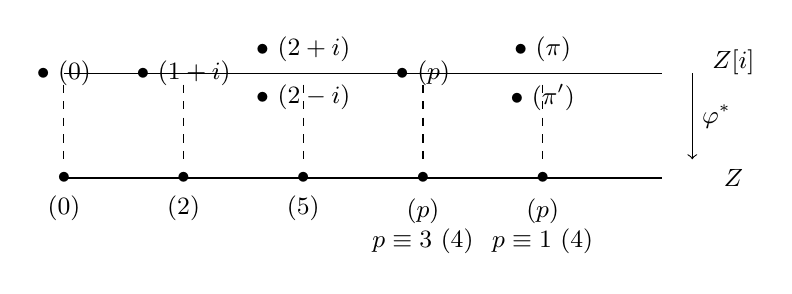
\begin{tikzpicture}[scale=0.95, every node/.style={font=\small}]
			\draw[->] (8.4,1.4) -- (8.4,0.25) node[midway,right] {$\varphi^*$};
			\node at (8.95,1.55) {$\Spec\mathbb Z[i]$};
			\node at (8.95,0) {$\Spec\mathbb Z$};
			\draw (0,1.4) -- (8,1.4);
			\draw (0,0) -- (8,0);
			\node at (0,1.4) {$\bullet\ (0)$};
			\node at (1.6,1.4) {$\bullet\ (1+i)$};
			\node at (3.2,1.72) {$\bullet\ (2+i)$};
			\node at (3.2,1.08) {$\bullet\ (2-i)$};
			\node at (4.8,1.4) {$\bullet\ (p)$};
			\node at (6.4,1.72) {$\bullet\ (\pi)$};
			\node at (6.4,1.08) {$\bullet\ (\pi')$};
			\node at (0,0) {$\bullet$}; \node[below=3pt] at (0,0) {$(0)$};
			\node at (1.6,0) {$\bullet$}; \node[below=3pt] at (1.6,0) {$(2)$};
			\node at (3.2,0) {$\bullet$}; \node[below=3pt] at (3.2,0) {$(5)$};
			\node at (4.8,0) {$\bullet$}; \node[below=3pt] at (4.8,0) {\begin{tabular}{c}$(p)$\\$p\equiv3\ (4)$\end{tabular}};
			\node at (6.4,0) {$\bullet$}; \node[below=3pt] at (6.4,0) {\begin{tabular}{c}$(p)$\\$p\equiv1\ (4)$\end{tabular}};
			\draw[dashed] (0,1.25)--(0,0.15);
			\draw[dashed] (1.6,1.25)--(1.6,0.15);
			\draw[dashed] (3.2,1.25)--(3.2,0.15);
			\draw[dashed] (4.8,1.25)--(4.8,0.15);
			\draw[dashed] (6.4,1.25)--(6.4,0.15);
		\end{tikzpicture}
	\end{center}
	
	\item 若 $k$ 是代数闭域，则 $\Spec k[x]$ 由 $(0)$ 以及理想 $(x-a)$（$a\in k$）组成；自然包含 $\varphi:k[x]\to k[x,y]$ 诱导 Zariski 连续映射
	\[
	\varphi^*:\Spec k[x,y]\longrightarrow\Spec k[x].
	\]
	$\Spec k[x,y]$ 的元素为
	\begin{enumerate}[label=(\alph*)]
		\item $(0)$；
		\item $(f)$，其中 $f$ 是 $k[x,y]$ 中的不可约多项式；
		\item $(x-a,y-b)$，其中 $a,b\in k$
	\end{enumerate}
	（参见练习 4）。素理想 $(0)$ 在 $\Spec k[x,y]$ 中 Zariski 稠密；(b) 中的素理想的 Zariski 闭包由 (c) 中满足 $f(a,b)=0$ 的素理想 $(x-a,y-b)$ 组成；闭点，也即 $\operatorname{mSpec}k[x,y]$ 的元素，是 (c) 中的素理想。
	
	由零点定理，$\Spec k[x,y]$ 中的每个素理想 $P$ 都由相应零点集 $Z(P)$ 唯一确定。素理想 $(0)\in k[x,y]$ 对应于 $\mathbb A^2$。素理想 $(f)$ 对应于满足 $f(x,y)=0$ 的点，而 $P=(f)$ 是包含 $P$ 的所有极大理想的交。极大理想 $(x-a,y-b)$ 对应于点 $(a,b)\in\mathbb A^2$。这些素理想在映射 $\varphi^*$ 下分布在 $\Spec k[x]$ 上，可以几何地画为下图：
	
	\begin{center}
		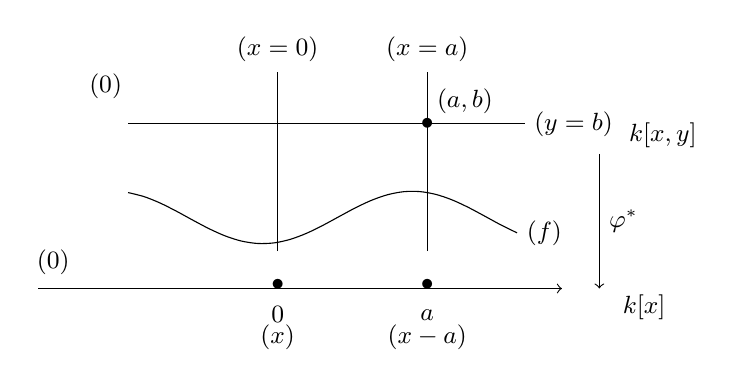
\begin{tikzpicture}[scale=0.95, every node/.style={font=\small}]
			\draw[->] (7.5,2.3) -- (7.5,0.5) node[midway,right] {$\varphi^*$};
			\node at (8.35,2.55) {$\Spec k[x,y]$};
			\node at (8.1,0.25) {$\Spec k[x]$};
			\draw[->] (0,0.5) -- (7,0.5);
			\node at (0.2,0.85) {$(0)$};
			\node at (3.2,0.15) {$0$};
			\node at (5.2,0.15) {$a$};
			\node at (3.2,0.55) {$\bullet$};
			\node at (5.2,0.55) {$\bullet$};
			\node[below] at (3.2,0.15) {$(x)$};
			\node[below] at (5.2,0.15) {$(x-a)$};
			\draw (3.2,1.0) -- (3.2,3.4) node[above] {$(x=0)$};
			\draw (5.2,1.0) -- (5.2,3.4) node[above] {$(x=a)$};
			\draw (1.2,2.7) -- (6.5,2.7) node[right] {$(y=b)$};
			\draw[domain=1.2:6.4,smooth,variable=\x] plot ({\x},{1.45+0.35*sin(90*\x)}) node[right] {$(f)$};
			\node at (5.2,2.7) {$\bullet$};
			\node[above right] at (5.2,2.7) {$(a,b)$};
			\node at (0.9,3.2) {$(0)$};
		\end{tikzpicture}
	\end{center}
	
	在这个图中，$\Spec k[x]$ 中的素理想 $(x-a)$ 被识别为元素 $a\in k$。$\Spec k[x,y]$ 中的素理想 $(x)$ 对应于 $\mathbb A^2$ 中满足 $x=0$ 的点，即对应于 $\mathbb A^2$ 中的 $y$-轴；素理想 $(y)\in\Spec k[x,y]$ 类似地对应于 $x$-轴。素理想 $(f)\in\Spec k[x,y]$ 对应于 $\mathbb A^2$ 中的不可约曲线 $f(x,y)=0$；这条曲线上的点 $(a,b)\in\mathbb A^2$ 对应于包含 $(f)$ 的极大理想 $(x-a,y-b)\in\Spec k[x,y]$。闭点 $(x-a,y-b)\in\Spec k[x,y]$ 对应于“几何点” $(a,b)\in\mathbb A^2$。
	
	注意，$\Spec k[x,y]$ 捕捉了 $\mathbb A^2$ 中代数集的全部几何：$\mathbb A^2$ 中每个代数集都是上图中 $\Spec k[x,y]$ 的元素所对应的某些不可约代数集的有限并。除处处稠密点 $(0)$ 以外，$\Spec k[x,y]$ 的“几何”图像正是仿射平面 $\mathbb A^2$ 的通常几何。若 $k$ 不是代数闭的，情形稍微复杂一些，但图像相似，参见练习 4。
	
	\item 把 $\Spec\mathbb Z[x]$ 看成由自然包含 $\mathbb Z\to\mathbb Z[x]$ 纤维化在 $\Spec\mathbb Z$ 上，其情形与前一例中 $\Spec k[x,y]$ 的情形非常类似。$\Spec\mathbb Z[x]$ 的元素已在命题 54 后的例 2 中讨论过，可画为下图：
	
	\begin{center}
		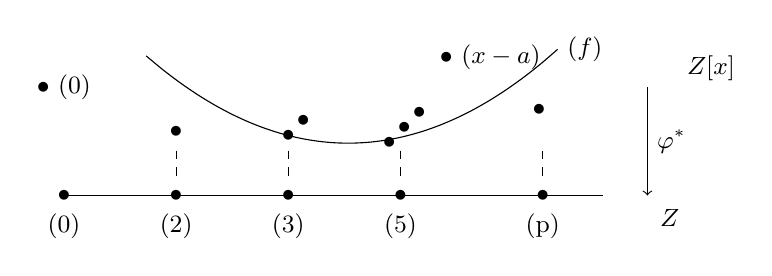
\begin{tikzpicture}[scale=0.95, every node/.style={font=\small}]
			\draw[->] (7.8,2.0) -- (7.8,0.55) node[midway,right] {$\varphi^*$};
			\node at (8.65,2.25) {$\Spec\mathbb Z[x]$};
			\node at (8.1,0.25) {$\Spec\mathbb Z$};
			\draw (0,0.55) -- (7.2,0.55);
			\foreach \x/\lab in {0/{(0)},1.5/{(2)},3/{(3)},4.5/{(5)},6.4/{(p)}}
			{\node at (\x,0.55) {$\bullet$}; \node[below=3pt] at (\x,0.55) {\lab};}
			\node at (0,2.0) {$\bullet\ (0)$};
			\draw[domain=1.1:6.6,smooth,variable=\x] plot ({\x},{1.25+0.16*(\x-3.8)*(\x-3.8)}) node[right] {$(f)$};
			\node at (5.7,2.4) {$\bullet\ (x-a)$};
			\node at (1.5,1.4) {$\bullet$};
			\node at (3.0,1.35) {$\bullet$};
			\node at (3.2,1.55) {$\bullet$};
			\node at (4.35,1.25) {$\bullet$};
			\node at (4.55,1.45) {$\bullet$};
			\node at (4.75,1.65) {$\bullet$};
			\node at (6.35,1.7) {$\bullet$};
			\draw[dashed] (1.5,1.15)--(1.5,0.72);
			\draw[dashed] (3,1.15)--(3,0.72);
			\draw[dashed] (4.5,1.15)--(4.5,0.72);
			\draw[dashed] (6.4,1.15)--(6.4,0.72);
		\end{tikzpicture}
	\end{center}
	
	元素 $(0)$ 在 $\Spec\mathbb Z[x]$ 中 Zariski 稠密。$(p)$ 的闭包由 $(p)$ 以及所有闭点 $(p,g)$ 组成，其中 $g$ 是 $\mathbb Z[x]$ 中模 $p$ 不可约的首一多项式。$(f)$ 的闭包由 $(f)$ 以及包含 $(f)$ 的极大理想 $(p,g)$ 组成，这等价于说 $f$ 在商环 $\mathbb Z[x]/(p,g)$ 中的像为 $0$，即不可约多项式 $g$ 是 $f$ 模 $p$ 的一个因子。闭点 $\operatorname{mSpec}\mathbb Z[x]$ 是极大理想 $(p,g)$。
	
	注意，包含 $(f)$ 的极大理想 $(p,g)$ 正是上图中 $\operatorname{mSpec}\mathbb Z[x]$ 中使 $\Spec\mathbb Z[x]$ 上的“函数” $f$ 为零的闭点，这里的函数把素理想 $P$ 送到
	\[
	f(P)=f\bmod P\in\mathbb Z[x]/P.
	\]
	例如，多项式
	\[
	f=x^3-4x^2+x-9\in\mathbb Z[x]
	\]
	符合上图：$f$ 在 $\mathbb Z[x]$ 中不可约，并且在 $\mathbb F_p$ 上分解成不可约因子的情形如下：
	\[
	\begin{aligned}
		f&=x^3+x+1\pmod 2,\\
		f&=x(x+1)^2\pmod 3,\\
		f&=(x+1)(x+2)(x+3)\pmod 5.
	\end{aligned}
	\]
	与 $(f)$ 相交且位于 $(2)$ 上方纤维中的点有一个，即闭点 $(2,x^3+x+1)$。位于 $(3)$ 上方纤维中的闭点有两个，分别为 $(3,x)$ 与 $(3,x+1)$（后一个点带有某种“重数”）。位于 $(5)$ 上方的闭点有三个：$(5,x+1)$、$(5,x+2)$ 与 $(5,x+3)$。在上图中，素数 $p$ 可以取 $p=53$，因为这是大于 $5$ 的第一个使此多项式模 $p$ 有三个不可约因子的素数。注意，虽然图中把素理想 $(f)$ 画成一条光滑曲线，以强调它与前一例中 $\Spec k[x,y]$ 结构的几何相似性，但 $\Spec\mathbb Z$ 中素数上方的纤维是离散的，因此应当谨慎。例如，由于
	\[
	f=(x+2)(x^2+x+6)\pmod 7,
	\]
	$(f)$ 与 $(7)$ 上方纤维的交只含有两个点 $(7,x+2)$ 与 $(7,x^2+x+6)$，每个重数为一。
	
	位于 $\Spec\mathbb Z$ 中 $(p)$ 上方纤维内的 $(f)$ 上的闭点可能个数由多项式 $f$ 在 $\mathbb Q$ 上的 Galois 群控制（参见第 14.8 节）。例如，$f=x^4+1$ 在 $(2)$ 上方纤维中有一个闭点，而对奇素数 $p$，在 $(p)$ 上方纤维中有两个或四个闭点（参见练习 8）。
\end{enumerate}

带有 Zariski 拓扑的空间 $\Spec R$，给出了任意交换环情形下对簇 $V$ 中点的几何推广。现在考虑如何推广 $V$ 上有理函数环的问题。

当 $V$ 是代数闭域 $k$ 上的簇时，坐标环 $k[V]$ 的商域 $k(V)$ 中的元素定义了 $V$ 上的有理函数。$k(V)$ 中每个元素 $\alpha$ 一般可以用许多不同方式写为 $a/f$，其中 $a,f\in k[V]$。$\alpha$ 正则的点的集合 $U$ 是 $V$ 的一个开子集；按定义，它由所有满足 $\alpha$ 可以表示成某个商 $a/f$ 且 $f(v)\ne0$ 的点 $v\in V$ 组成，此时代表元 $a/f$ 定义了局部环 $\mathcal O_{v,V}$ 中的元素。还要注意，同一个代表元 $a/f$ 不仅在 $v$ 处定义 $\alpha$，而且在 $f$ 非零的所有点上都定义 $\alpha$，即在 $V$ 的开子集
\[
V_f=\{w\in V\mid f(w)\ne0\}
\]
上定义。这些开集 $V_f$（称为主开集，参见第 2 节练习 21）随着 $\alpha$ 的各种可能代表元 $a/f$ 而给出 $U$ 的一个开覆盖。命题 51 前的例子中，$V=Z(xz-yw)\subseteq\mathbb A^4$ 上函数 $\alpha=x/y$ 表明，一般情况下，单个代表元并不足以确定整个 $U$；在这个例子中，$U=V_y\cup V_z$，而 $U$ 不能由任何单个 $V_f$ 覆盖（参见第 4 节练习 25）。

把有理函数理解为某些开子集上的正则函数，这一解释可以推广到 $\Spec R$。我们首先定义 $X=\Spec R$ 中集合 $V_f$ 的类似物 $X_f$，并建立其基本性质。

\noindent\textbf{定义.} 对任意 $f\in R$，令 $X_f$ 表示 $X=\Spec R$ 中不包含 $f$ 的素理想的集合。等价地，$X_f$ 是 $\Spec R$ 中元素 $f\in R$ 的值非零的点的集合。集合 $X_f$ 称为 $\Spec R$ 中的\emph{主开集}（或\emph{基本开集}）。

由于 $X_f$ 是 Zariski 闭集 $Z(f)$ 的补集，所以它确实是 $\Spec R$ 中的开集，正如名称所示。下面的命题列出主开集的一些基本性质。回忆，拓扑空间之间的映射称为同胚，如果它连续、双射且逆映射也连续。

\noindent\textbf{命题 56.} 设 $f\in R$，并设 $X_f$ 是 $X=\Spec R$ 中相应的主开集。则：
\begin{enumerate}[label=(\arabic*)]
	\item $X_f=X$ 当且仅当 $f$ 是单位，而 $X_f=\varnothing$ 当且仅当 $f$ 是幂零元；
	\item $X_f\cap X_g=X_{fg}$；
	\item $X_f\subseteq X_{g_1}\cup\cdots\cup X_{g_n}$ 当且仅当
	\[
	f\in\operatorname{rad}(g_1,\ldots,g_n);
	\]
	特别地，$X_f=X_g$ 当且仅当 $\operatorname{rad}(f)=\operatorname{rad}(g)$；
	\item 主开集构成 $\Spec R$ 上 Zariski 拓扑的一组基，即 $X$ 的每个 Zariski 开集都是某些主开集 $X_f$ 的并；
	\item 从 $R$ 到 $R_f$ 的自然映射诱导一个从 $\Spec R_f$ 到 $X_f$ 的同胚，其中 $R_f$ 是 $R$ 在 $f$ 处的局部化；
	\item 任意环的谱都是拟紧的（即每个开覆盖都有有限子覆盖）；特别地，$X_f$ 是拟紧的；
	\item 若 $\varphi:R\to S$ 是任意环同态（且 $\varphi(1_R)=1_S$），则在诱导映射
	\[
	\varphi^*:Y=\Spec S\longrightarrow\Spec R
	\]
	下，$X$ 中主开集 $X_f$ 的全逆像是 $Y$ 中的主开集 $Y_{\varphi(f)}$。
\end{enumerate}

\begin{proof}
	(1)、(2) 与 (7) 留作简单练习。为证明 (3)，注意根据定义，$X_{g_1}\cup\cdots\cup X_{g_n}$ 由那些不包含 $g_1,\ldots,g_n$ 中至少一个元素的素理想 $P$ 组成。因此 $X_{g_1}\cup\cdots\cup X_{g_n}$ 是闭集 $Z((g_1,\ldots,g_n))$ 的补集，其中后者由包含理想 $(g_1,\ldots,g_n)$ 的素理想 $P$ 组成。若 $(g_1,\ldots,g_n)=R$，则 $X_{g_1}\cup\cdots\cup X_{g_n}=X$，无须证明。否则，$X_f\subseteq X_{g_1}\cup\cdots\cup X_{g_n}$ 当且仅当每个满足 $f\notin P$ 的素理想 $P$ 也满足 $P\notin Z((g_1,\ldots,g_n))$。后一条件等价于说：如果素理想 $P$ 包含理想 $(g_1,\ldots,g_n)$，则 $P$ 也包含 $f$；即 $f$ 属于所有包含 $(g_1,\ldots,g_n)$ 的素理想 $P$ 的交。由命题 12，这个交为 $\operatorname{rad}(g_1,\ldots,g_n)$，从而证明 (3)。
	
	若 $U=X-Z(I)$ 是 $X$ 的一个 Zariski 开子集，则 $U$ 是所有 $X_f$（$f\in I$）的并，这证明 (4)。
	
	从 $R$ 到局部化 $R_f$ 的自然环同态建立了 $R_f$ 中素理想与 $R$ 中不包含 $(f)$ 的素理想之间的一一对应（命题 38）。因此，从 $\Spec R_f$ 到 $\Spec R$ 的相应 Zariski 连续映射是连续双射。由于 $R_f$ 的每个理想都是 $R$ 的某个理想的扩张（参见命题 38(1)），可知逆映射也连续，这证明 (5)。
	
	对 (6)，由 (4) 每个开集都是主开集的并，因此只需证明：若 $X$ 被主开集 $X_{g_i}$（$i$ 属于某个指标集 $\mathcal J$）覆盖，则 $X$ 是其中有限多个 $X_{g_i}$ 的并。若由所有 $g_i$ 生成的理想 $I$ 是 $R$ 的真理想，则 $I$ 包含于某个极大理想 $P$ 中。但这时 $X=\Spec R$ 中的点 $P$ 不属于任何主开集 $X_{g_i}$，与 $X$ 被这些 $X_{g_i}$ 覆盖相矛盾。因此 $I=R$，所以 $1\in R$ 可写为有限和
	\[
	1=a_1g_{i_1}+\cdots+a_ng_{i_n}
	\]
	其中 $i_1,\ldots,i_n\in\mathcal J$。考虑有限并 $X_{g_{i_1}}\cup\cdots\cup X_{g_{i_n}}$。若 $X$ 中某点 $P$ 不属于这个并，则 $P$ 是 $R$ 中包含 $g_{i_1},\ldots,g_{i_n}$ 的素理想，从而包含 $1$，矛盾。因此
	\[
	X=X_{g_{i_1}}\cup\cdots\cup X_{g_{i_n}},
	\]
	如所需。(6) 的第二部分由 (5) 推出。
\end{proof}

现在我们为 $X=\Spec R$ 定义簇 $V$ 上有理函数的类似物。如前所见，对簇 $V$，有理函数 $\alpha\in k(V)$ 是某个开集 $U$ 上的正则函数。在每个点 $v\in U$ 处，存在 $\alpha$ 的代表元 $a/f$ 且 $f(v)\ne0$；这个代表元是局部化
\[
\mathcal O_{v,V}=k[V]_{I(v)}
\]
中的元素。这样，$U$ 上的正则函数 $\alpha$ 可以看作从 $U$ 到这些局部化的不交并的函数：点 $v\in U$ 被映到代表元 $a/f\in k[V]_{I(v)}$。此外，同一个代表元不仅可以在 $v$ 处使用，也可以在 $v$ 的整个 Zariski 邻域 $V_f$ 上同时使用（所以“在 $v$ 附近局部地”，$\alpha$ 由 $k[V]$ 中元素的单个商给出）。注意，$a/f$ 是局部化 $k[V]_f$ 中的元素，而后者包含于所有 $w\in V_f$ 的局部化 $k[V]_{I(w)}$ 中。

现在我们把这推广到 $\Spec R$。考虑从 $\Spec R$ 的 Zariski 开子集 $U$ 到局部化 $R_P$（$P\in U$）的不交并的函数 $s$ 的集合，要求 $s(P)\in R_P$，并且 $s$ 局部地由 $R$ 中元素的商给出。更精确地说：

\noindent\textbf{定义.} 设 $U$ 是 $\Spec R$ 的 Zariski 开子集。若 $U=\varnothing$，定义 $\mathcal O(U)=0$。否则，定义 $\mathcal O(U)$ 为所有函数
\[
s:U\longrightarrow\coprod_{Q\in U}R_Q
\]
的集合，其中 $s$ 从 $U$ 到 $Q\in U$ 的局部化 $R_Q$ 的不交并，并且满足如下两个性质：
\begin{enumerate}[label=(\arabic*)]
	\item 对每个 $Q\in U$，有 $s(Q)\in R_Q$；
	\item 对每个 $P\in U$，存在 $P$ 在 $U$ 中的一个开邻域 $X_f\subseteq U$ 以及局部化 $R_f$ 中的一个元素 $a/f^n$，在 $X_f$ 上定义 $s$，即对每个 $Q\in X_f$，有
	\[
	s(Q)=a/f^n\in R_Q.
	\]
\end{enumerate}

若 $s,t$ 是 $\mathcal O(U)$ 的元素，则 $s+t$ 与 $st$ 也都是 $\mathcal O(U)$ 的元素（参见练习 18），所以每个 $\mathcal O(U)$ 都是一个环。此外，每个 $a\in R$ 定义了 $\mathcal O(U)$ 中的一个元素，即 $s(Q)=a\in R_Q$；特别地，$1\in R$ 给出了环 $\mathcal O(U)$ 的单位元。若 $U'$ 是 $U$ 的一个开子集，则存在从 $\mathcal O(U)$ 到 $\mathcal O(U')$ 的自然限制映射，它是环同态（参见练习 19）。

\noindent\textbf{定义.} 设 $R$ 是含 $1$ 的交换环，并令 $X=\Spec R$。
\begin{enumerate}[label=(\arabic*)]
	\item 对 $X$ 的 Zariski 开集 $U$ 给出的环 $\mathcal O(U)$ 以及当 $U'\subseteq U$ 时的限制映射 $\mathcal O(U)\to\mathcal O(U')$，称为 $X$ 上的\emph{结构层}，简单记作 $\mathcal O$（或 $\mathcal O_X$）。
	\item $\mathcal O(U)$ 的元素 $s$ 称为 $\mathcal O$ 在 $U$ 上的\emph{截面}。$\mathcal O(X)$ 的元素称为 $\mathcal O$ 的\emph{整体截面}。
\end{enumerate}

下一个命题推广了命题 51 的结果：簇 $V$ 上处处正则的有理函数恰好是坐标环 $k[V]$ 的元素。

\noindent\textbf{命题 57.} 设 $X=\Spec R$，并设 $\mathcal O=\mathcal O_X$ 是其结构层。$\mathcal O$ 的整体截面就是 $R$ 的元素，即
\[
\mathcal O(X)\simeq R.
\]
更一般地，若 $X_f$ 是 $X$ 中由某个 $f\in R$ 给出的主开集，则 $\mathcal O(X_f)$ 同构于局部化 $R_f$。

\begin{proof}
	设 $a/f^r$ 是局部化 $R_f$ 的一个元素。则由
	\[
	s(Q)=a/f^r\in R_Q,
	\qquad Q\in X_f,
	\]
	定义的映射给出 $\mathcal O(X_f)$ 中的一个元素；显然得到的映射
	\[
	\psi:R_f\longrightarrow\mathcal O(X_f)
	\]
	是环同态。假设对每个 $Q\in X_f$，有 $a/f^r=b/f^s$ 在 $R_Q$ 中成立，即存在某个 $g\notin Q$ 使得
	\[
	g(af^s-bf^r)=0
	\]
	在 $R$ 中成立。令 $I$ 为 $R$ 中所有满足
	\[
	x(af^s-bf^r)=0
	\]
	的元素 $x$ 组成的理想。由 $g\in I$ 可知，对任意 $Q\in X_f$，$I$ 不包含于 $Q$。换句话说，$R$ 中每个包含 $I$ 的素理想也包含 $f$。因此 $f$ 属于所有包含 $I$ 的素理想的交，也就是说 $f\in\operatorname{rad}I$。于是对某个整数 $N\ge0$，有 $f^N\in I$，所以
	\[
	f^N(af^s-bf^r)=0
	\]
	在 $R$ 中成立。这说明 $a/f^r=b/f^s$ 在 $R_f$ 中成立，因此映射 $\psi$ 是单射。
	
	现在设 $s\in\mathcal O(X_f)$。根据定义，$X_f$ 可以被主开集 $X_{g_i}$ 覆盖，在每个 $X_{g_i}$ 上，对每个 $Q\in X_{g_i}$，有
	\[
	s(Q)=a_i/g_i^{n_i}\in R_Q.
	\]
	由命题 56(6)，可以取有限多个 $g_i$；再通过改变 $a_i$，可以假设所有 $n_i$ 都相等（因为若 $n$ 是所有 $n_i$ 的最大值，则
	\[
	a_i/g_i^{n_i}=(a_ig_i^{n-n_i})/g_i^n
	\]
	）。由于对所有 $Q\in X_{g_ig_j}=X_{g_i}\cap X_{g_j}$，有
	\[
	s(Q)=a_i/g_i^n=a_j/g_j^n\in R_Q,
	\]
	把单射性应用于 $R_{g_ig_j}$ 可知
	\[
	a_i/g_i^n=a_j/g_j^n\quad\text{在 }R_{g_ig_j}\text{ 中}.
	\]
	这意味着对某个 $N\ge0$，有
	\[
	(g_ig_j)^N(a_ig_j^n-a_jg_i^n)=0,
	\]
	即
	\[
	a_i g_j^{n+N}g_i^N=a_j g_i^{n+N}g_j^N
	\]
	在 $R$ 中成立；可以假设 $N$ 充分大，使得这个等式对每一对 $i,j$ 都成立。
	
	由于 $X_f$ 是 $X_{g_i}=X_{g_i^{n+N}}$ 的并，由命题 56(3)，$f$ 属于由 $g_i^{n+N}$ 生成的理想的根。于是存在 $M\ge1$ 与 $b_i\in R$，使得
	\[
	f^M=\sum_i b_i g_i^{n+N}.
	\]
	定义
	\[
	a=\sum_i b_i a_i g_i^N\in R.
	\]
	于是
	\[
	g_j^N a_j f^M
	=\sum_i b_i(a_j g_i^{n+N}g_j^N)
	=\sum_i b_i(a_i g_i^N g_j^{n+N})
	=g_j^{n+N}a.
	\]
	因此 $a/f^M=a_j/g_j^n$ 在 $R_{g_j}$ 中成立。所以由 $R_f$ 中元素 $a/f^M$ 定义的 $\mathcal O(X_f)$ 中的元素，在每个 $X_{g_j}$ 上都与 $s$ 相同；由于这些开集覆盖 $X_f$，它在整个 $X_f$ 上与 $s$ 相同。因此映射 $\psi$ 给出同构
	\[
	R_f\simeq\mathcal O(X_f).
	\]
	取 $f=1$ 得 $R\simeq\mathcal O(X)$，证明完毕。
\end{proof}

在仿射簇 $V$ 的情形中，点 $v\in V$ 处的局部环 $\mathcal O_{v,V}$ 是 $k(V)$ 中在 $v$ 处有定义的所有有理函数的集合。换句话说，$\mathcal O_{v,V}$ 是所有包含 $v$ 的开集 $U$ 上正则函数环的并，其中这个并是在 $V$ 的函数域 $k(V)$ 中取的。在更一般的情形 $X=\Spec R$ 中，包含 $P\in\Spec R$ 的开集上的环 $\mathcal O(U)$ 并不包含在如此显然的公共环中。在这种情况下，我们考虑所有对 $(s,U)$ 的集合，其中 $U$ 是包含 $P$ 的 $X$ 的开集且 $s\in\mathcal O(U)$。如果存在包含 $P$ 的开集 $U''\subseteq U\cap U'$，使得 $s$ 与 $s'$ 限制到 $\mathcal O(U'')$ 后相同，则把两个对 $(s,U)$ 与 $(s',U')$ 视为等价。在仿射簇的情形中，这就是说，在点 $v$ 的 Zariski 邻域中定义的两个函数，如果在 $v$ 的某个公共邻域中相同，则它们在 $v$ 处定义同一个正则函数。这些等价类组成的集合定义了环 $\mathcal O(U)$ 的正向极限，记作 $\varinjlim_P\mathcal O(U)$（参见第 7.6 节练习 8）。

\noindent\textbf{定义.} 若 $P\in X=\Spec R$，则所有包含 $P$ 的 $X$ 的开集 $U$ 上的环 $\mathcal O(U)$ 的正向极限
\[
\varinjlim_P\mathcal O(U)
\]
称为结构层在 $P$ 处的\emph{茎}，记作 $\mathcal O_P$。

\noindent\textbf{命题 58.} 设 $X=\Spec R$，并设 $\mathcal O=\mathcal O_X$ 是其结构层。$\mathcal O$ 在点 $P\in X$ 处的茎同构于 $R$ 在 $P$ 处的局部化 $R_P$：
\[
\mathcal O_P\simeq R_P.
\]
特别地，茎 $\mathcal O_P$ 是局部环。

\begin{proof}
	若 $(s,U)$ 代表茎 $\mathcal O_P$ 中的一个元素，则 $s(P)$ 是局部化 $R_P$ 的一个元素。由正向极限的定义，这个元素不依赖于代表元 $(s,U)$ 的选择，因此给出从 $\mathcal O_P$ 到 $R_P$ 的良定义环同态 $\phi$。若 $a,f\in R$ 且 $f\notin P$，则映射
	\[
	s(Q)=a/f\in R_Q
	\]
	定义了 $\mathcal O(X_f)$ 中的一个元素。那么 $(s,X_f)$ 在茎 $\mathcal O_P$ 中的等价类在 $\phi$ 下被映到 $R_P$ 中的 $a/f$，所以 $\phi$ 是满射。
	
	为说明 $\phi$ 也是单射，设 $\mathcal O_P$ 中 $(s,U)$ 与 $(s',U')$ 的等价类满足
	\[
	s(P)=s'(P)\quad\text{在 }R_P\text{ 中}.
	\]
	由 $\mathcal O(U)$ 的定义，在某个 $g\notin P$ 的 $X_g$ 上，$s=a/g^n$。类似地，在某个 $g'\notin P$ 的 $X_{g'}$ 上，$s'=b/(g')^m$。由于
	\[
	a/g^n=b/(g')^m\quad\text{在 }R_P\text{ 中},
	\]
	存在某个 $h\notin P$，使得
	\[
	h(a(g')^m-bg^n)=0
	\]
	在 $R$ 中成立。若 $Q\in X_{gg'h}=X_g\cap X_{g'}\cap X_h$，这个等式说明
	\[
	a/g^n=b/(g')^m\quad\text{在 }R_Q\text{ 中}.
	\]
	因此 $s$ 与 $s'$ 限制到 $X_{gg'h}$ 后相同。由正向极限的定义，$(s,U)$ 与 $(s',U')$ 在茎 $\mathcal O_P$ 中定义同一个元素。这证明 $\phi$ 是单射，从而证明命题。
\end{proof}

命题 58 表明，对 $P\in\Spec R$ 代数地定义的局部化 $R_P$ 起到了仿射簇 $V$ 上点 $v$ 处正则函数局部环 $\mathcal O_{v,V}$ 的作用。若 $\mathfrak m_P$ 表示 $R_P$ 中的极大理想 $PR_P$，并且
\[
k(P)=R_P/\mathfrak m_P
\]
表示相应的商域（由命题 46(1)，它也是 $R/P$ 的分式域），则 $P$ 处的切空间定义为 $k(P)$-向量空间 $\mathfrak m_P/\mathfrak m_P^2$ 的对偶。这是一个代数定义，它推广了簇 $V$ 在点 $v$ 处切空间 $T_{v,V}$ 的定义（由命题 52）。现在可以用它来定义 $\Spec R$ 中的点非奇异是什么意思：点 $P\in\Spec R$ 称为\emph{非奇异}或\emph{光滑}的，如果局部环 $R_P$ 是所谓的“正则局部环”（参见第 16.2 节）。

命题 58 还提示了结构层在 $\Spec R$ 上的一个漂亮几何图像。如果把每个点 $P\in\Spec R$ 看成其上方有局部环 $R_P$，那么在 $X=\Spec R$ 的开集 $U$ 上方，就有这些“茎”的一个“层”（这里的“层”可理解为“丛”，而“茎”可理解为“麦秆的茎”），这有助于解释一些术语。结构层 $\mathcal O(U)$ 中的一个截面 $s$ 是从 $U$ 到这些茎所成丛的映射。下图中阴影区域表示这样一个截面 $s$ 在 $U$ 下的像。

\begin{center}
	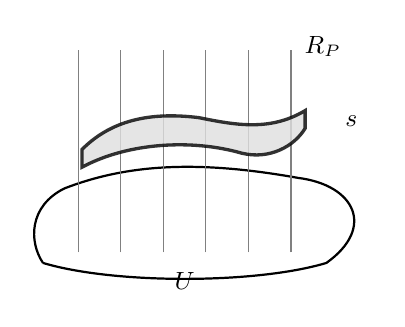
\begin{tikzpicture}[scale=0.9, every node/.style={font=\small}]
		\draw[thick] (0,0) .. controls (1,-0.3) and (3,-0.3) .. (4,0)
		.. controls (4.7,0.5) and (4.4,1.1) .. (3.6,1.2)
		.. controls (2.2,1.45) and (1.2,1.4) .. (0.3,1.05)
		.. controls (-0.2,0.8) and (-0.2,0.3) .. (0,0);
		\node at (2,-0.25) {$U$};
		\foreach \x in {0.5,1.1,1.7,2.3,2.9,3.5}
		\draw[gray] (\x,0.15) -- (\x,3.0);
		\draw[very thick, fill=gray!25, opacity=0.8] (0.55,1.35) .. controls (1.2,1.7) and (2.1,1.75) .. (2.8,1.55) .. controls (3.2,1.45) and (3.55,1.65) .. (3.7,1.9) -- (3.7,2.15) .. controls (3.2,1.85) and (2.7,1.95) .. (2.2,2.05) .. controls (1.4,2.15) and (0.9,1.95) .. (0.55,1.6) -- cycle;
		\node at (4.35,2.0) {$s$};
		\node at (3.95,3.05) {$R_P$};
	\end{tikzpicture}
\end{center}

\noindent\textbf{定义.} 设 $R$ 是含 $1$ 的交换环。有序对
\[
(\Spec R,\mathcal O_{\Spec R}),
\]
即带有 Zariski 拓扑的空间 $\Spec R$ 连同结构层 $\mathcal O_{\Spec R}$，称为一个\emph{仿射概形}。

仿射概形的概念给出了仿射代数集几何对任意交换环完全代数化的推广，并且是现代代数几何的出发点。

\paragraph{例}
\begin{enumerate}[label=(\arabic*)]
	\item 若 $F$ 是任意域，则 $X=\Spec F=\{(0)\}$。在这种情形下只有两个开集 $X$ 与 $\varnothing$，它们都是主开集：$X=X_1$ 且 $\varnothing=X_0$。整体截面为 $\mathcal O(X)=F$。只有一个茎：$\mathcal O_{(0)}=F_{(0)}=F$。
	
	\item 若 $R=\mathbb Z$，则由于 $R$ 是 P.I.D.，$X=\Spec\mathbb Z$ 的每个开集都是主开集：
	\[
	X_n=\{(p)\mid p\nmid n\}
	\]
	并且
	\[
	\mathcal O(X_n)=\mathbb Z_n=\mathbb Z[1/n]
	=\left\{a/b\in\mathbb Q\mid \text{若素数 }p\mid b\text{，则 }p\mid n\right\}.
	\]
	对非零素数 $p$，$(p)$ 处的茎是局部环 $\mathbb Z_{(p)}$；$(0)$ 处的茎是 $\mathbb Q$。所有限制映射以及从截面到茎的映射都是自然包含。
	
	\item 对一般整环 $R$，设其商域为 $F$，则茎与截面为
	\[
	\mathcal O(U)=\{a/b\in F\mid b\notin P\text{ 对所有 }P\in U\text{ 成立}\},
	\]
	\[
	\mathcal O_P=R_P=\{a/b\in F\mid b\notin P\},
	\]
	其中 $(0)$ 处的茎是 $F$，即 $\mathcal O_{(0)}=F$。同样，限制映射以及到茎的映射都是包含。
	
	\item 对局部环
	\[
	R=\mathbb Z_{(2)}=\{a/b\in\mathbb Q\mid b\text{ 为奇数}\},
	\]
	有 $\Spec R=\{(0),(2)\}$，其中 $(2)$ 是唯一闭点，且 $\{(0)\}=X_2$ 是主开集。截面 $\mathcal O(\{(0)\})$ 为 $R_2=\mathbb Q$，茎为
	\[
	\mathcal O_{(0)}=R_{(0)}=\mathbb Q,
	\qquad
	\mathcal O_{(2)}=R_{(2)}=R.
	\]
\end{enumerate}

接下来考虑由环同态 $R\to S$ 所产生的对应于 $R$ 与 $S$ 的仿射概形之间的关系。

设 $\varphi:R\to S$ 是一个环同态。我们已在命题 56(7) 中看到，存在诱导连续映射
\[
\varphi^*:Y=\Spec S\longrightarrow X=\Spec R,
\]
并且在此映射下，对 $g\in R$，主开集 $X_g$ 的全逆像是主开集 $Y_{\varphi(g)}$。由此可知，$\varphi$ 也诱导相应截面上的映射，如下所述。设 $Q'\in Y$ 是 $\Spec S$ 的任意元素，并设
\[
Q=\varphi^*(Q')=\varphi^{-1}(Q')\in X
\]
是 $\Spec R$ 中对应的元素。若 $U$ 是 $X$ 中包含 $Q$ 的 Zariski 开集，则
\[
U'=(\varphi^*)^{-1}(U)
\]
是 $Y$ 中包含 $Q'$ 的 Zariski 开集。注意，$\varphi$ 诱导一个自然环同态（记为 $\varphi_Q$）从局部化 $R_Q$ 到局部化 $S_{Q'}$，定义为
\[
\varphi_Q(a/f)=\varphi(a)/\varphi(f)\in S_{Q'}
\]
其中 $f\notin Q$。设 $s\in\mathcal O_X(U)$ 是 $X$ 的结构层的一个截面，并且在 $P\in X$ 的邻域 $X_g$ 中局部由 $a/g^n$ 给出。容易检查复合
\[
s':U'\longrightarrow U\longrightarrow\coprod_{Q\in U}R_Q
\longrightarrow\coprod_{Q'\in U'}S_{Q'}
\]
定义了一个映射，它在邻域 $Y_{\varphi(g)}$ 中局部由元素 $\varphi(a)/\varphi(g)^n$ 给出；因此 $s'\in\mathcal O_Y(U')$ 是 $Y$ 的结构层的一个截面。于是可以直接检查，所得映射
\[
\varphi^\#:\mathcal O_X(U)\longrightarrow\mathcal O_Y(U')
\]
是环同态（把 $\mathcal O_X(U)$ 中的 $1$ 映到 $\mathcal O_Y(U')$ 中的 $1$），并且与 $\mathcal O_X$ 与 $\mathcal O_Y$ 上的限制映射相容（参见练习 20）。同时还得到茎上的诱导环同态：对任意点 $P'\in\Spec S$ 以及对应点 $P=\varphi^*(P')\in\Spec R$，有
\[
\varphi^\#: \mathcal O_{X,P}\longrightarrow\mathcal O_{Y,P'}.
\]
在命题 58 的同构下，从 $R_P\simeq\mathcal O_{X,P}$ 到 $S_{P'}\simeq\mathcal O_{Y,P'}$ 的同态 $\varphi^\#$ 正是由同态 $\varphi$ 诱导出的局部化上的自然环同态 $\varphi_P$。特别地，在 $\varphi^\#$ 下，局部环 $\mathcal O_{Y,P'}$ 中极大理想的逆像是局部环 $\mathcal O_{X,P}$ 中的极大理想。

\noindent\textbf{定义.} 设 $(\Spec R,\mathcal O_{\Spec R})$ 与 $(\Spec S,\mathcal O_{\Spec S})$ 是两个仿射概形。从 $(\Spec S,\mathcal O_{\Spec S})$ 到 $(\Spec R,\mathcal O_{\Spec R})$ 的\emph{仿射概形态射}是一个有序对 $(\varphi^*,\varphi^\#)$，满足：
\begin{enumerate}[label=(\arabic*)]
	\item $\varphi^*:\Spec S\to\Spec R$ 是 Zariski 连续的；
	\item 对 $\Spec R$ 的每个 Zariski 开子集 $U$，都有环同态
	\[
	\varphi^\#:\mathcal O(U)\longrightarrow\mathcal O((\varphi^*)^{-1}(U)),
	\]
	并且这些同态与限制映射交换；
	\item 若 $P'\in\Spec S$ 且对应点 $P=\varphi^*(P')\in\Spec R$，则在茎上的诱导同态
	\[
	\varphi^\#: \mathcal O_{\Spec R,P}\longrightarrow \mathcal O_{\Spec S,P'}
	\]
	下，$\mathcal O_{\Spec S,P'}$ 的极大理想的逆像是 $\mathcal O_{\Spec R,P}$ 的极大理想。
\end{enumerate}

从局部环 $A$ 到局部环 $B$ 的同态 $\psi:A\to B$，如果具有 $B$ 的极大理想的逆像为 $A$ 的极大理想这一性质，则称为局部环的\emph{局部同态}。上述定义中的第三个条件就是要求茎上的诱导同态为局部同态。

用这个术语，定义前的讨论说明，一个环同态 $\varphi:R\to S$ 诱导一个从 $(\Spec S,\mathcal O_{\Spec S})$ 到 $(\Spec R,\mathcal O_{\Spec R})$ 的仿射概形态射。

反过来，设 $(\varphi^*,\varphi^\#)$ 是从 $(\Spec S,\mathcal O_{\Spec S})$ 到 $(\Spec R,\mathcal O_{\Spec R})$ 的一个仿射概形态射。特别地，对 $U=\Spec R$，有 $(\varphi^*)^{-1}(U)=\Spec S$；因此按假设，在整体截面上存在环同态
\[
\varphi^\#: \mathcal O_{\Spec R}(\Spec R)
\longrightarrow
\mathcal O_{\Spec S}(\Spec S).
\]
由命题 57，有环同构
\[
\mathcal O_{\Spec R}(\Spec R)\simeq R,
\qquad
\mathcal O_{\Spec S}(\Spec S)\simeq S.
\]
与这些同构复合说明，$\varphi^\#$ 给出一个环同态 $\varphi:R\to S$。由命题 58，我们有一个局部同态 $\varphi^\#:R_P\to S_{P'}$；并且由它与限制同态的相容性可知，下图交换：
\[
\begin{array}{ccc}
	R & \xrightarrow{\varphi} & S\\
	\downarrow & & \downarrow\\
	R_P & \xrightarrow{\varphi^\#} & S_{P'}
\end{array}
\]
其中两个竖直映射是自然局部化同态。由于假设 $\varphi^\#$ 是局部同态，
\[
(\varphi^\#)^{-1}(P'S_{P'})=PR_P,
\]
由此推出 $\varphi^{-1}(P')=P$。因此，由 $\varphi$ 诱导的从 $\Spec S$ 到 $\Spec R$ 的连续映射与 $\varphi^*$ 相同；并且容易推出 $\varphi$ 也如前所述诱导同态 $\varphi^\#$。这说明存在环同态 $\varphi:R\to S$，同时诱导出 $\varphi^*$ 与 $\varphi^\#$。

我们把这概括为如下定理。

\noindent\textbf{定理 59.} 每个环同态 $\varphi:R\to S$ 都诱导一个仿射概形态射
\[
(\varphi^*,\varphi^\#):(\Spec S,\mathcal O_{\Spec S})
\longrightarrow
(\Spec R,\mathcal O_{\Spec R}).
\]
反过来，每个仿射概形态射都来自这样的一个环同态 $\varphi$。

定理 59 是 $\Spec R$ 情形中定理 6 的类似物；定理 6 把仿射代数集之间的几何问题转化为其坐标环的代数问题。

在仿射概形态射的定义中，要求茎上的同态是局部同态这一条件是必要的：谱上的连续映射连同一组截面上的相容环同态（因而也诱导茎上的同态），并不足以迫使这些映射来自某个环同态。

\paragraph{例}
令 $R=\mathbb Z_{(2)}$ 且 $S=\mathbb Q$，如前面的一组例子所述。定义
\[
\varphi^*:\Spec\mathbb Q\longrightarrow\Spec\mathbb Z_{(2)}
\]
为 $\varphi^*((0))=(2)$（它是 Zariski 连续的）。定义
\[
\varphi^\#:\mathcal O(\Spec R)\longrightarrow\mathcal O(\Spec S)
\]
为包含映射 $\mathbb Z_{(2)}\to\mathbb Q$，并且对所有其他 $U\subseteq\Spec R$ 简单地定义 $\varphi^\#$ 为零映射。直接检查可知，这些同态与限制映射交换。然而，这一族映射并不来自一个环同态，因为对 $(0)\in\Spec S$ 以及 $\varphi^*((0))=(2)\in\Spec R$ 的茎而言，诱导同态
\[
\varphi^\#:\mathcal O_{\Spec R,(2)}\longrightarrow\mathcal O_{\Spec S,(0)}
\]
是包含映射 $\mathbb Z_{(2)}\to\mathbb Q$，它不是局部同态（$(0)$ 的逆像是 $(0)$，而不是极大理想 $2\mathbb Z_{(2)}$）。

定理 59 的证明说明，一个仿射概形态射 $(\varphi^*,\varphi^\#)$ 必然来自 $\varphi^\#$ 在整体截面上定义的环同态。在本例中，整体截面上的同态是 $R$ 到 $S$ 的包含映射。从 $R$ 到 $S$ 的包含映射定义了从 $\Spec S$ 到 $\Spec R$ 的映射，它把 $\Spec S$ 中的 $(0)$ 映到 $\Spec R$ 中的 $(0)$，而不是映到 $\Spec R$ 中的 $(2)$，所以这个映射不同于原来的映射 $\varphi^*$。

前一例说明，如果没有仿射概形态射定义中的第三个（局部同态）条件，定理 59 的逆命题就不成立。由此，定理 59 表明，观察仿射概形的适当背景是局部环空间的范畴。粗略地说，一个\emph{局部环空间}是一个拓扑空间 $X$，连同对 $X$ 的每个开子集 $U$ 给出的一族环 $\mathcal O(U)$（当 $U'\subseteq U$ 时有从 $\mathcal O(U)$ 到 $\mathcal O(U')$ 的相容同态，并且截面满足某些局部条件），使得对 $P\in U$，茎
\[
\mathcal O_P=\varinjlim_P\mathcal O(U)
\]
是局部环。这个范畴中的态射是拓扑空间之间的连续映射，连同相应 $\mathcal O(U)$ 之间的环同态，并满足与仿射概形态射定义中所施加条件完全相同的条件。

一个\emph{概形}是一个局部环空间，其中每个点都位于一个与仿射概形同构的邻域中（并且这些邻域之间还满足某些相容条件），它是现代代数几何中的基本研究对象。这里考虑的仿射概形是构造一般概形时“粘合”在一起的构件，正如通常的 Euclidean 空间是在分析中定义流形时被“粘合”在一起的构件一样。

\subsection*{练习}

所有环均假定为含幺交换环，所有环同态均假定保持恒等元。

\begin{enumerate}[label=\arabic*.]
	\item 若 $N$ 是 $R$ 的 nilradical，证明 $\Spec R$ 与 $\Spec R/N$ 同胚。[说明从 $R$ 到 $R/N$ 的自然同态诱导从 $\Spec R/N$ 到 $\Spec R$ 的 Zariski 连续同构。]
	
	\item 设 $I$ 是环 $R$ 中的理想。证明由典范投影同态 $R\to R/I$ 诱导的连续映射从 $\Spec R/I$ 到 $\Spec R$，把 $\Spec R/I$ 同胚地映到 $\Spec R$ 中的闭集 $Z(I)$ 上。
	
	\item 证明两个元素 $f,g\in R$ 在 $\Spec R$ 中所有元素 $P$ 处的值相同，当且仅当 $f-g$ 属于 $R$ 的 nilradical。特别地，证明仿射 $k$-代数中的元素由其取值唯一确定。
	
	\item 设 $k$ 是任意域，不必代数闭。证明 $k[x,y]$ 中的素理想（即 $\Spec k[x,y]$ 的元素）为
	\begin{enumerate}[label=(\roman*)]
		\item $(0)$；
		\item $(f)$，其中 $f$ 是 $k[x,y]$ 中的不可约多项式；
		\item $(p(x),g(x,y))$，其中 $p(x)$ 是 $k[x]$ 中的不可约多项式，而 $g(x,y)$ 是 $k[x,y]$ 中的不可约多项式，并且模 $p(x)$ 后仍不可约，即 $g(x,y)$ 在商环 $k[x,y]/(p(x))$ 中仍不可约。
	\end{enumerate}
	证明 $\operatorname{mSpec}k[x,y]$ 由 (iii) 中的素理想组成。[使用第 1 节练习 20。]
	
	\item 令 $\mathfrak m=(p(x),g(x,y))$ 是前一练习中的 $k[x,y]$ 的极大理想。说明 $K=k[x,y]/\mathfrak m$ 是 $k$ 的代数域扩张，从而 $k[x,y]$ 也可看成 $K[x,y]$ 的子环。若在典范同态 $k[x,y]\to k[x,y]/\mathfrak m$ 下，$x,y$ 分别映到 $\alpha,\beta\in K$，证明
	\[
	\mathfrak m=k[x,y]\cap (x-\alpha,y-\beta)
	\]
	其中 $(x-\alpha,y-\beta)\subseteq K[x,y]$。
	
	\item 描述 $\Spec\mathbb R[x]$ 与 $\Spec\mathbb C[x]$ 中的元素。描述 $\Spec\mathbb Z_{(2)}[x]$ 中的元素，其中
	\[
	\mathbb Z_{(2)}=\{a/b\in\mathbb Q\mid b\text{ 为奇数}\}
	\]
	是 $\mathbb Z$ 在素理想 $(2)$ 处的局部化。
	
	\item 令 $(f)=(x^5+x+1)$ 为 $\Spec\mathbb Z[x]$ 中的点，并把它看成如命题 55 后例 3 那样纤维化在 $\Spec\mathbb Z$ 上。说明在 $(2)$ 上方纤维中有两个闭点，在 $(5)$ 上方纤维中有三个闭点，在 $(19)$ 上方纤维中有四个闭点，在 $(211)$ 上方纤维中有五个闭点。
	
	\item 令 $(f)=(x^4+1)$ 为 $\Spec\mathbb Z[x]$ 中的点，并把它看成如命题 55 后例 3 那样纤维化在 $\Spec\mathbb Z$ 上。证明在 $(2)$ 上方纤维中有一个闭点；当 $p$ 为奇素数且 $p\equiv1\pmod 8$ 时，在 $p$ 上方纤维中有四个闭点；而对所有其他奇素数 $p$，在 $p$ 上方纤维中有两个闭点（参见第 14 章第 3 节推论 16）。
	
	\item 证明从 $\Spec\mathbb Z[x]$ 到 $\Spec\mathbb Z$ 的 Zariski 连续映射在 $(p)$ 上方的纤维中的元素，与
	\[
	\Spec(\mathbb Z[x]\otimes_{\mathbb Z}\mathbb F_p)
	\]
	中的元素同胚。
	
	\item 设 $X=\Spec R$，并设 $X_f$ 是对应于 $f\in R$ 的主开集。证明
	\[
	X_f\cap X_g=X_{fg}.
	\]
	证明 $X_f=X$ 当且仅当 $f$ 是 $R$ 中的单位，并且 $X_f=\varnothing$ 当且仅当 $f$ 是幂零元。
	
	\item 若 $X_f$ 与 $X_g$ 是 $X=\Spec R$ 中的主开集，证明开集 $X_f\cup X_g$ 是闭集 $Z(I)$ 的补集，其中 $I=(f,g)$ 是 $R$ 中由 $f$ 与 $g$ 生成的理想。
	
	\item 证明 $X=\Spec R$ 的 Zariski 开子集 $U$ 是拟紧的，当且仅当 $U$ 是有限多个主开子集的并。给出一个环 $R$、$\Spec R$ 的一个 Zariski 开子集 $U$，以及 $U$ 的一个不能缩减为有限子覆盖的 Zariski 开覆盖的例子。
	
	\item 设 $\varphi:R\to S$ 是环同态。证明在诱导映射 $\varphi^*$ 从 $Y=\Spec S$ 到 $X=\Spec R$ 下，$X$ 中主开集 $X_f$ 的全逆像是 $Y$ 中的主开集 $Y_{\varphi(f)}$。
	
	\item 设 $R=R_1\times R_2$ 是环 $R_1$ 与 $R_2$ 的直积。证明 $X=\Spec R$ 是两个开子空间 $X_1,X_2$ 的不交并（因此它们也都是闭的），其中 $X_1$ 同胚于 $\Spec R_1$，$X_2$ 同胚于 $\Spec R_2$。
	
	\item 证明 $X=\Spec R$ 不连通，当且仅当 $R$ 是两个非零环的直积，当且仅当 $R$ 含有一个满足 $e\ne0,1$ 的幂等元 $e$（参见前一练习）。
	
	\item 证明 $X=\Spec R$ 是不可约的（即任意两个非空开子集都有非平凡交），当且仅当任意两个非空主开集 $X_f$ 与 $X_g$ 都满足 $X_f\cap X_g\ne\varnothing$。推出 $X=\Spec R$ 不可约当且仅当 $R$ 的 nilradical 是素理想。[使用练习 10。]
	
	\item 令 $G=\langle a\rangle$ 是 $2$ 阶群，令
	\[
	R=\mathbb Z[G]=\{m+na\mid m,n\in\mathbb Z\}
	\]
	是相应的群环，并令 $X=\Spec R$。
	\begin{enumerate}[label=(\alph*)]
		\item 证明 $R$ 的 nilradical 是 $(0)$，但它不是素理想。证明
		\[
		X=X^+\cup X^- ,
		\]
		其中 $X^+=Z(1-a)$ 且 $X^-=Z(1+a)$。[使用 $(1+a)(1-a)=0$。]
		
		\item 证明同态 $\mathbb Z[G]\to\mathbb Z$，由把 $a$ 映到 $1$ 定义，诱导 $X^+$ 与 $\Spec\mathbb Z$ 的一个同胚；而由把 $a$ 映到 $-1$ 定义的同态诱导 $X^-$ 与 $\Spec\mathbb Z$ 的一个同胚。
		
		\item 证明 $X^+\cap X^-$ 由单个元素
		\[
		\mathfrak m=(1+a,1-a)=(2,1-a)
		\]
		组成，并且这是 $X$ 中的闭点。
		
		\item 说明 $(1-a)$ 与 $(1+a)$ 是 $X$ 中唯一的非闭点，其闭包分别为 $X^+$ 与 $X^-$。描述 $X$ 中的闭点 $\operatorname{mSpec}R$，并证明 $\Spec\mathbb Z[\langle a\rangle]$ 可以画为下图：
		
		\begin{center}
			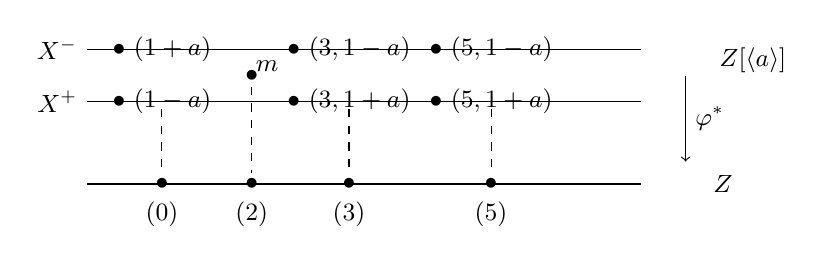
\begin{tikzpicture}[scale=0.95, every node/.style={font=\small}]
				\draw[->] (8.0,1.45) -- (8.0,0.3) node[midway,right] {$\varphi^*$};
				\node at (8.9,1.65) {$\Spec\mathbb Z[\langle a\rangle]$};
				\node at (8.5,0) {$\Spec\mathbb Z$};
				\draw (0,1.8) -- (7.4,1.8);
				\draw (0,1.1) -- (7.4,1.1);
				\node[left] at (0,1.8) {$X^-$};
				\node[left] at (0,1.1) {$X^+$};
				\node at (1.0,1.8) {$\bullet\ (1+a)$};
				\node at (1.0,1.1) {$\bullet\ (1-a)$};
				\node at (3.5,1.8) {$\bullet\ (3,1-a)$};
				\node at (3.5,1.1) {$\bullet\ (3,1+a)$};
				\node at (5.4,1.8) {$\bullet\ (5,1-a)$};
				\node at (5.4,1.1) {$\bullet\ (5,1+a)$};
				\node at (2.2,1.45) {$\bullet$};
				\node[above right=-2pt] at (2.2,1.45) {$\mathfrak m$};
				\draw (0,0) -- (7.4,0);
				\foreach \x/\lab in {1/{(0)},2.2/{(2)},3.5/{(3)},5.4/{(5)}}
				{\node at (\x,0) {$\bullet$}; \node[below=3pt] at (\x,0) {\lab};}
				\draw[dashed] (1.0,1.0)--(1.0,0.15);
				\draw[dashed] (2.2,1.3)--(2.2,0.15);
				\draw[dashed] (3.5,1.0)--(3.5,0.15);
				\draw[dashed] (5.4,1.0)--(5.4,0.15);
			\end{tikzpicture}
		\end{center}
	\end{enumerate}
	
	\item 设 $\mathcal O$ 是 $X=\Spec R$ 上的结构层，设 $U$ 是 $X$ 中开集，并设 $s,t\in\mathcal O(U)$。若在 $X_{f_1}$ 上有 $s=a/f_1^n$，在 $X_{f_2}$ 上有 $t=b/f_2^m$，说明在 $X_{f_1f_2}$ 上有
	\[
	st=\frac{ab}{(f_1f_2)^{n+m}}\,f_1^m f_2^n
	\]
	按通常写法即
	\[
	st=\frac{abf_1^m f_2^n}{(f_1f_2)^{n+m}},
	\qquad
	s+t=\frac{af_2^{m+n}+bf_1^{m+n}}{(f_1f_2)^{n+m}}.
	\]
	推出 $\mathcal O(U)$ 是含单位元的交换环。
	
	\item 设 $\mathcal O$ 是 $X=\Spec R$ 上的结构层，设 $V\subseteq U$ 是 $X$ 中开集，并设 $s\in\mathcal O(U)$。假设 $P\in V$，且在 $X_f\subseteq U$ 上有 $s=a/f^n$。
	\begin{enumerate}[label=(\alph*)]
		\item 说明存在包含 $P$ 的主开集 $X_{f'}\subseteq V\cap X_f$。
		\item 说明对某个 $b\in R$，有 $(f')^m=bf$。
		\item 说明在 $X_{f'}$ 上有
		\[
		s=\frac{ab^n}{(f')^{mn}},
		\]
		并推出把 $s$ 限制到 $V$ 给出从 $\mathcal O(U)$ 到 $\mathcal O(V)$ 的良定义环同态。
	\end{enumerate}
	
	\item 设 $\varphi:R\to S$ 是环同态，设 $X=\Spec R$，$Y=\Spec S$，并设 $V\subseteq U$ 是 $X$ 的 Zariski 开子集。令
	\[
	V'=(\varphi^*)^{-1}(V),
	\qquad
	U'=(\varphi^*)^{-1}(U),
	\]
	它们是关于由 $\varphi$ 诱导的连续映射 $\varphi^*:Y\to X$ 的 $Y$ 中对应 Zariski 开子集。证明截面上的诱导映射
	\[
	\varphi^\#:\mathcal O_X(U)\longrightarrow\mathcal O_Y(U')
	\]
	是环同态。证明 $V'\subseteq U'$，并且 $\varphi^\#$ 与限制映射相容，即图
	\[
	\begin{array}{ccc}
		\mathcal O_X(U)&\xrightarrow{\varphi^\#}&\mathcal O_Y(U')\\
		\downarrow&&\downarrow\\
		\mathcal O_X(V)&\xrightarrow{\varphi^\#}&\mathcal O_Y(V')
	\end{array}
	\]
	交换，其中竖直映射为限制同态。
	
	\item 设 $D$ 是 $R$ 的乘法闭子集。说明局部化同态 $R\to D^{-1}R$ 诱导一个从 $\Spec(D^{-1}R)$ 到所有满足 $P\cap D=\varnothing$ 的 $R$ 中素理想 $P$ 所组成集合的同胚。
	
	\item 说明 $\Spec k[x,y]/(xy)$ 是连通的，但它是两个真闭子集的并，且每个都同胚于 $\Spec k[x]$；因此它不是不可约的（参见练习 16）。
	
	\item 对下列每个环 $R$，列出 $\Spec R$ 的元素、$\Spec R$ 中的开集 $U$、对每个开集 $U$ 结构层在 $U$ 上的截面 $\mathcal O(U)$，以及每个点 $P\in\Spec R$ 处的茎 $\mathcal O_P$：
	\[
	\text{(a) }\mathbb Z/4\mathbb Z,
	\quad
	\text{(b) }\mathbb Z/6\mathbb Z,
	\quad
	\text{(c) }\mathbb Z/2\mathbb Z\times\mathbb Z/3\mathbb Z,
	\quad
	\text{(d) }\mathbb Z/2\mathbb Z\times\mathbb Z/2\mathbb Z\times\mathbb Z/2\mathbb Z.
	\]
	
	\item \begin{enumerate}[label=(\alph*)]
		\item 若 $R$ 的每个理想都是主理想，说明 $\Spec R$ 中每个开集都是主开集。
		\item 说明若
		\[
		R=\mathbb Z[x]/(4,x^2),
		\]
		则 $R$ 含有非主理想，但 $\Spec R$ 中每个开集仍是主开集。
	\end{enumerate}
	
	\item \begin{enumerate}[label=(\alph*)]
		\item 若 $M$ 是 $R$-模，证明 $\operatorname{Supp}(M)$ 是 $\Spec R$ 的 Zariski 闭子集。[使用第 4 节练习 33。]
		\item 若 $M$ 是有限生成 $R$-模，证明
		\[
		\operatorname{Supp}(M)=Z(\operatorname{Ann}(M))\subseteq\Spec R.
		\]
		[使用第 4 节练习 34。]
	\end{enumerate}
	
	\item 设 $M$ 是 Noether 环 $R$ 上的有限生成模。
	\begin{enumerate}[label=(\alph*)]
		\item 证明包含 $\operatorname{Ann}(M)$ 的极小素理想只有有限多个，设为 $P_1,\ldots,P_n$。[使用推论 22。]
		\item 证明 $\{P_1,\ldots,P_n\}$ 也是 $\operatorname{Ass}_R(M)$ 中极小素理想的集合，并且 $\operatorname{Supp}(M)$ 是 $\Spec R$ 中 Zariski 闭集
		\[
		Z(P_1),\ldots,Z(P_n)
		\]
		的并。[使用前一练习与第 4 节练习 40。]
	\end{enumerate}
	
	前一练习给出了 Noether 环 $R$ 上有限生成模 $M$ 的几何图像：在 $\Spec R$ 中每个点 $P$ 上方是局部化 $M_P$（$P$ 上方的茎）。这个茎恰好在 Zariski 闭子集 $Z(P_1),\ldots,Z(P_n)$ 上方的点处非零，其中 $P_i$ 是 $\operatorname{Ass}_R(M)$ 中的极小素理想。这些思想导向了 $\Spec R$ 上与 $M$ 相关的（凝聚）模层的概念（其图像类似于命题 58 后结构层的图像），这是现代代数几何中的一个有力工具。
	
	\item 令 $R=k[x,y]$，并令 $M$ 为 $R$ 中的理想 $(x,y)$。证明
	\[
	\operatorname{Supp}(M)=\Spec R
	\qquad\text{且}\qquad
	\operatorname{Ass}_R(M)=\{0\}.
	\]
	
	下面两个练习说明，在 Noether 环 $R$ 中，对理想 $I$ 而言，primary 分解意义下的相关素理想正是 $\operatorname{Ass}_R(R/I)$ 意义下的相关素理想。
	
	\item 本练习证明 Noether 环 $R$ 中理想 $Q$ 是 $P$-primary 的，当且仅当
	\[
	\operatorname{Ass}_R(R/Q)=\{P\}.
	\]
	\begin{enumerate}[label=(\alph*)]
		\item 设 $Q$ 是 $P$-primary 理想，并令 $M$ 为 $R$-模 $R/Q$。若 $0\ne m\in M$，说明
		\[
		Q\subseteq\operatorname{Ann}(m)\subseteq P,
		\qquad
		\operatorname{rad}\operatorname{Ann}(m)=P.
		\]
		推出若 $\operatorname{Ann}(m)$ 是素理想，则它等于 $P$，从而
		\[
		\operatorname{Ass}_R(R/Q)=\{P\}.
		\]
		[使用第 1 节练习 33。]
		
		\item 对 $R$ 的任意理想 $Q$，设 $0\ne M\subseteq R/Q$。证明 $\operatorname{Ann}(M)$ 的根是 $\operatorname{Supp}(M)$ 中素理想的交。[使用命题 12 与练习 25。]
		
		\item 对 (b) 中的 $M$，证明 $\operatorname{Ann}M$ 的根也等于 $\operatorname{Ass}_R(M)$ 中素理想的交。[使用练习 26(b)。]
		
		\item 若 $Q$ 是 $R$ 的理想且 $\operatorname{Ass}_R(R/Q)=\{P\}$，证明 $\operatorname{rad}Q=P$。[使用 $Q=\operatorname{Ann}(R/Q)$ 以及 (c)。]
		
		\item 若 $Q$ 是 $R$ 的理想且 $\operatorname{Ass}_R(R/Q)=\{P\}$，证明 $Q$ 是 $P$-primary。[若 $ab\in Q$ 且 $a\notin Q$，考虑
		\[
		0\ne M=(Ra+Q)/Q\subseteq R/Q,
		\]
		并说明 $b$ 属于 $\operatorname{Ann}M\subseteq\operatorname{rad}\operatorname{Ann}(M)$。使用第 1 节练习 33--34 说明 $\operatorname{Ass}_R(M)=\{P\}$，再用 (c) 说明 $\operatorname{rad}\operatorname{Ann}(M)=P$，最后推出 $b\in P$。]
	\end{enumerate}
	
	\item 设
	\[
	I=Q_1\cap\cdots\cap Q_n
	\]
	是 Noether 环 $R$ 中理想 $I$ 的一个极小 primary 分解，并设
	\[
	P_i=\operatorname{rad}Q_i,
	\qquad i=1,\ldots,n.
	\]
	本练习证明
	\[
	\operatorname{Ass}_R(R/I)=\{P_1,\ldots,P_n\}.
	\]
	\begin{enumerate}[label=(\alph*)]
		\item 证明自然投影同态诱导一个从 $R/I$ 到
		\[
		R/Q_1\oplus\cdots\oplus R/Q_n
		\]
		的单射，并推出
		\[
		\operatorname{Ass}_R(R/I)\subseteq\{P_1,\ldots,P_n\}.
		\]
		[使用第 1 节练习 34 以及前一练习。]
		
		\item 令
		\[
		Q_i'=\bigcap_{j\ne i}Q_j.
		\]
		说明分解的极小性蕴含
		\[
		0\ne Q_i'/I=(Q_i'+Q_i)/Q_i\subseteq R/Q_i.
		\]
		推出
		\[
		\operatorname{Ass}_R(Q_i'/I)=\{P_i\}.
		\]
		[使用第 1 节练习 33--34 以及前一练习。] 推出 $\{P_i\}\in\operatorname{Ass}_R(R/I)$，从而
		\[
		\operatorname{Ass}_R(R/I)=\{P_1,\ldots,P_n\}.
		\]
		[使用 $Q_i'/I\subseteq R/I$ 以及第 1 节练习 34。]
	\end{enumerate}
	
	\item 令 $I$ 是 $R=k[x,y,z]$ 中的理想
	\[
	I=(x^2,xy,xz,yz).
	\]
	证明 $\operatorname{Ass}_R(R/I)$ 由素理想
	\[
	\{(x,y),(x,z),(x,y,z)\}
	\]
	组成。
	
	\item （二次整数环的素谱）令 $R$ 为二次域 $K=\mathbb Q(\sqrt D)$ 的整数环，其中 $D$ 是无平方因子的整数；令 $P$ 是 $R$ 的非零素理想。本练习说明如何由 $\mathbb Z$ 中的素理想 $(p)$ 明确确定 $R$ 中的素理想，从而特别给出 $\Spec R$ 在 $\Spec\mathbb Z$ 上的纤维描述。
	
	如定理 29 后的讨论与例子所述，有 $R=\mathbb Z[\omega]$，其中若 $D\equiv2,3\pmod 4$，则 $\omega=\sqrt D$；而若 $D\equiv1\pmod 4$，则 $\omega=(1+\sqrt D)/2$。其极小多项式分别为
	\[
	m_\omega(x)=x^2-D,
	\]
	或
	\[
	m_\omega(x)=x^2-x+\frac{1-D}{4},
	\]
	并且 $P\cap\mathbb Z=p\mathbb Z$ 是 $\mathbb Z$ 的非零素理想。
	\begin{enumerate}[label=(\alph*)]
		\item 对 $\mathbb Z$ 中任意素数 $p$，证明环同构
		\[
		R/pR\simeq \mathbb Z[x]/(p,m_\omega(x))
		\simeq\mathbb F_p[x]/(\overline{m_\omega}(x)),
		\]
		其中 $\overline{m_\omega}(x)$ 是 $m_\omega(x)$ 模 $p$ 的化简。推出存在 $R$ 中素理想 $P$，满足 $P\cap\mathbb Z=(p)$（这在本情形下给出定理 26(2) 的另一个证明）。
		
		\item 使用 (a) 中的同构，证明 $P$ 可由 $m_\omega(x)$ 模 $p$ 的分解显式确定：
		\begin{enumerate}[label=(\roman*)]
			\item 若
			\[
			m_\omega(x)=(x-a)^2\pmod p,
			\]
			其中 $a\in\mathbb Z$，则
			\[
			P=(p,\omega-a),
			\qquad
			pR=P^2.
			\]
			说明这种情形只会发生在有限多个素数 $p$ 上，即那些整除 $m_\omega(x)$ 判别式的素数。
			
			\item 若
			\[
			m_\omega(x)=(x-a)(x-b)\pmod p,
			\]
			其中整数 $a,b\in\mathbb Z$ 模 $p$ 不同，则 $P$ 或者是
			\[
			P_1=(p,\omega-a),
			\]
			或者是
			\[
			P_2=(p,\omega-b),
			\]
			且 $P_1,P_2$ 是 $R$ 中不同的素理想，并满足
			\[
			pR=P_1P_2.
			\]
			
			\item 若 $m_\omega(x)$ 模 $p$ 不可约，则
			\[
			P=pR.
			\]
		\end{enumerate}
		
		\item 说明对任意 $D$，$\Spec R$ 在 $\Spec\mathbb Z$ 上方的图像都类似于 $D=-1$ 时 $R=\mathbb Z[i]$ 的情形：在 $\Spec\mathbb Z$ 中 $(0)$ 上方，$\Spec R$ 中恰有一个非闭点 $(0)$；对 (i) 中的素数 $(p)$（称为 ramified primes）以及 (iii) 中的素数（称为 inert primes），其上方在 $\Spec R$ 中恰有一个闭点 $P$；对 (ii) 中的素数（称为 split primes），其上方恰有两个闭点。
	\end{enumerate}
\end{enumerate}

